\documentclass[11pt,oneside]{book}
\usepackage{fontspec}
\setmainfont{Noto Serif}
\setsansfont{Noto Sans}
\setmonofont{Noto Sans Mono}
\newfontfamily\proseunicodefont{DejaVu Serif}
\usepackage[margin=1in]{geometry}
\usepackage{microtype}
\usepackage{amsmath,amssymb,amsthm,mathtools,bm}
\usepackage{graphicx}
\usepackage{xcolor}
\usepackage{booktabs}
\usepackage{array}
\usepackage{longtable}
\usepackage{enumitem}
\usepackage{float}
\usepackage{caption}
\usepackage{hyperref}
\usepackage{fancyhdr}
\usepackage{tikz}
\usetikzlibrary{arrows.meta,positioning,calc,decorations.pathmorphing}

\hypersetup{
  colorlinks=true,
  linkcolor=blue!50!black,
  urlcolor=blue!50!black,
  citecolor=blue!50!black
}

\setlength{\parskip}{0.5em}
\setlength{\parindent}{0pt}
\setlist[itemize]{topsep=0.25em,itemsep=0.2em}
\setlist[enumerate]{topsep=0.25em,itemsep=0.2em}
\setlength{\headheight}{40pt}
\numberwithin{equation}{chapter}

\newtheorem{theorem}{Teorema}[chapter]
\newtheorem{proposition}[theorem]{Proposición}
\newtheorem{lemma}[theorem]{Lema}
\newtheorem{corollary}[theorem]{Corolario}
\theoremstyle{definition}
\newtheorem{definition}[theorem]{Definición}
\newtheorem{example}[theorem]{Ejemplo}
\theoremstyle{remark}
\newtheorem{remark}[theorem]{Observación}

\providecommand{\ket}[1]{\left\lvert#1\right\rangle}
\providecommand{\bra}[1]{\left\langle#1\right\rvert}
\providecommand{\braket}[2]{\left\langle#1\,\middle|\,#2\right\rangle}
\providecommand{\expect}[1]{\left\langle#1\right\rangle}
\newcommand{\lectureoverview}[1]{\paragraph{Resumen.} #1}

\makeatletter
\newcommand{\course@headerfont}{\normalfont\small\itshape}
\newcommand{\course@pagefont}{\normalfont\small}
\newcommand{\course@headerraise}{14pt}
\newlength{\course@headerboxheight}
\setlength{\course@headerboxheight}{\dimexpr\headheight-\course@headerraise-9pt\relax}
\newcommand{\course@leftheadbox}[1]{%
  \raisebox{\course@headerraise}{%
    \parbox[t][\course@headerboxheight][t]{0.82\textwidth}{%
      \raggedright\course@headerfont\strut\MakeUppercase{#1}\strut%
    }%
  }%
}
\newcommand{\course@rightheadbox}[1]{%
  \raisebox{\course@headerraise}{%
    \parbox[t][\course@headerboxheight][t]{0.82\textwidth}{%
      \raggedleft\course@headerfont\strut\MakeUppercase{#1}\strut%
    }%
  }%
}
\renewcommand{\chaptermark}[1]{\markboth{\MakeUppercase{\chaptername\ \thechapter.\ #1}}{}}
\renewcommand{\sectionmark}[1]{\markright{\MakeUppercase{\thesection\hspace{0.4em}#1}}}
\fancyhf{}
\fancyhead[L]{\course@leftheadbox{\leftmark}}
\fancyhead[R]{\course@pagefont\thepage}
\renewcommand{\headrulewidth}{0.5pt}
\pagestyle{fancy}
\fancypagestyle{plain}{%
  \fancyhf{}
  \fancyhead[L]{\course@leftheadbox{\leftmark}}
  \fancyhead[R]{\course@pagefont\thepage}
  \renewcommand{\headrulewidth}{0.5pt}
}
\makeatother

% Video2Book editorial provenance macros
\newenvironment{classroomqa}{%
  \par\medskip\noindent\begin{minipage}{\linewidth}\small\hrule\medskip
}{%
  \medskip\hrule\end{minipage}\par\medskip
}
\newcommand{\audiencequestion}[1]{\noindent\textbf{Pregunta del público.} #1\par\smallskip}
\newcommand{\lecturerresponse}[1]{\noindent\textbf{Respuesta.} #1\par}
\newcommand{\lecturetimestamp}[1]{\footnote{Marca temporal: #1.}}
\newcommand{\lectureframe}[1]{\par\smallskip{\centering\footnotesize\itshape Fotograma de la clase: #1.\par}}
\newcommand{\editorialnote}[1]{\footnote{Aclaración editorial: #1}}

\usepackage{polyglossia}
\setdefaultlanguage{spanish}
\usepackage{sectsty}
\renewcommand{\contentsname}{Índice}
\renewcommand{\chaptername}{Capítulo}
\renewcommand{\figurename}{Figura}
\renewcommand{\tablename}{Tabla}
\renewcommand{\proofname}{Demostración}
\renewcommand{\bibname}{Bibliografía}
\sectionfont{\raggedright}
\subsectionfont{\raggedright}
\makeatletter
\renewcommand{\@pnumwidth}{2.2em}
\renewcommand{\@tocrmarg}{3.2em}
\makeatother
\usepackage{tocloft}
\renewcommand{\cftchapfont}{\small\bfseries}
\renewcommand{\cftchappagefont}{\small\bfseries}
\renewcommand{\cftsecfont}{\small}
\renewcommand{\cftsecpagefont}{\small}
\setlength{\cftsecnumwidth}{3em}
\renewcommand{\cftsubsecfont}{\small}
\renewcommand{\cftsubsecpagefont}{\small}
\setlength{\cftsubsecindent}{4.5em}
\setlength{\cftsubsecnumwidth}{4em}
\emergencystretch=6em
\pdfstringdefDisableCommands{\def\proseunicodefont{}}

\geometry{paperwidth=177.6mm,paperheight=252mm,left=16mm,right=16mm,
 top=18mm,bottom=18mm,includeheadfoot,headheight=28pt,headsep=7mm,footskip=9mm}
\usepackage{scrextend}
\changefontsizes[17pt]{12pt}
\raggedbottom
\renewenvironment{classroomqa}{\par\medskip\begingroup}{\par\endgroup\medskip}
\fancyhf{}
\setlength{\headwidth}{\textwidth}
\fancyhead[L]{\parbox{\textwidth}{\raggedright\fontsize{9}{11}\selectfont\nouppercase{\leftmark}}}
\fancyfoot[C]{\small\thepage}
\renewcommand{\headrulewidth}{0.3pt}
\fancypagestyle{plain}{\fancyhf{}\fancyfoot[C]{\small\thepage}\renewcommand{\headrulewidth}{0pt}}

\graphicspath{{../../../generated_course_notes/core/cosmology/2009_winter_legacy_cosmology/figures/}{../../../generated_course_notes/core/cosmology/2009_winter_legacy_cosmology/assets/}}
\begin{document}
\frontmatter
\hypersetup{pageanchor=false}
\begin{titlepage}
\hyphenpenalty=10000\exhyphenpenalty=10000
\thispagestyle{empty}
\begin{tikzpicture}[remember picture,overlay]
  \node[anchor=center,inner sep=0] at (current page.center) {%
    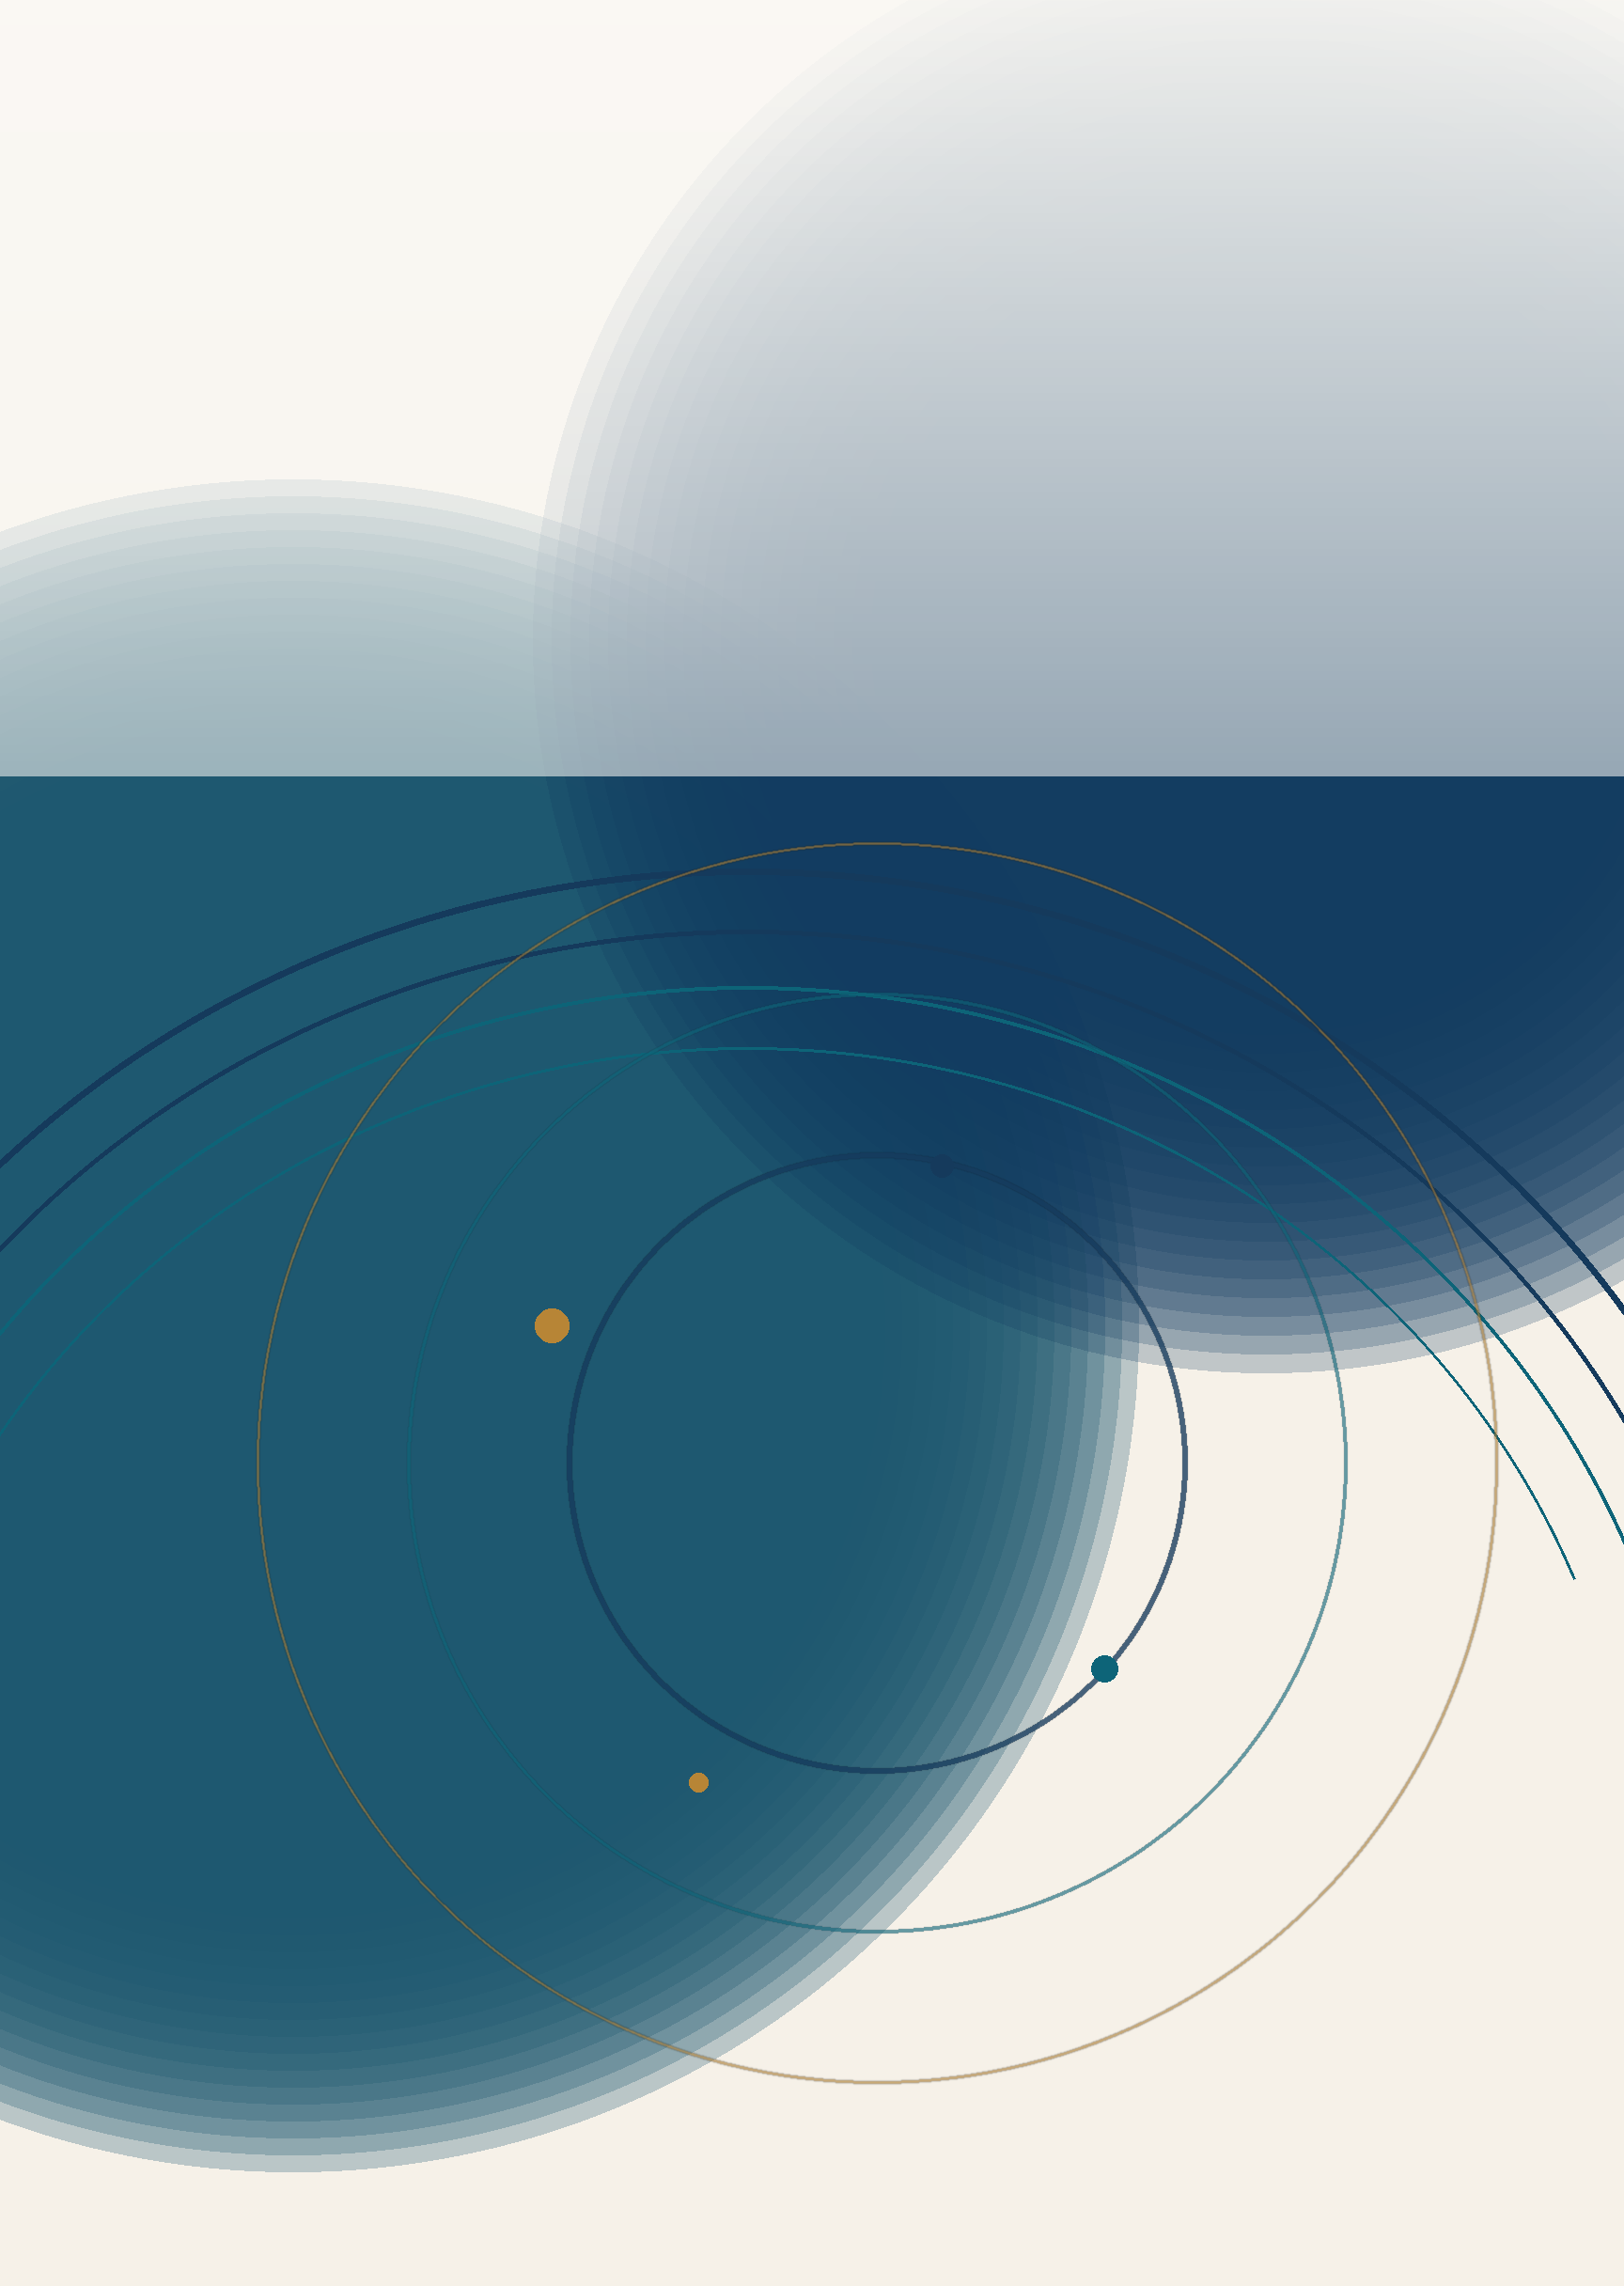
\includegraphics[height=\paperheight,keepaspectratio]{../../../generated_course_notes/core/cosmology/2009_winter_legacy_cosmology/assets/cover-art.png}%
  };
  \node[
    anchor=north west,
    align=left,
    text width=0.78\paperwidth,
    fill=white,
    fill opacity=0.9,
    rounded corners=8pt,
    inner xsep=10pt,
    inner ysep=8pt
  ] at ([xshift=0.08\paperwidth,yshift=-0.06\paperheight]current page.north west) {%
    {\fontsize{30}{33}\selectfont\bfseries\color{black!88} Cosmología\\[0.85em]}
    {\large\color{black!72} Edición en español / invierno de 2009, curso anterior de cosmología}
  };
  \node[
    anchor=south west,
    align=left,
    text width=0.68\paperwidth,
    fill=white,
    fill opacity=0.82,
    text opacity=1,
    rounded corners=6pt,
    inner sep=12pt
  ] at ([xshift=0.08\paperwidth,yshift=0.08\paperheight]current page.south west) {%
    {\normalsize\color{black!78} Clases originales: Leonard Susskind\\[0.35em]}
    {\small\color{black!72} Edición complementaria: \href{https://lazying.art}{LazyingArt LLC} / \href{https://github.com/lachlanchen/Video2Book}{Video2Book}}
  };
\end{tikzpicture}
\mbox{}
\end{titlepage}
\hypersetup{pageanchor=true}

\clearpage
\chapter*{Sobre estas notas}
Estas notas complementarias, editadas de forma independiente, acompañan las clases de Leonard Susskind. Se reconstruyeron a partir de transcripciones automáticas, subtítulos y una selección de fotogramas de la pizarra, y luego se cotejaron con el material fuente disponible. No son un manuscrito original del profesor Susskind ni han sido revisadas ni aprobadas por él.

La edición fue preparada por \href{https://lazying.art}{LazyingArt LLC} mediante el flujo de trabajo de código abierto \href{https://github.com/lachlanchen/Video2Book}{Video2Book}. Las transcripciones automáticas siguen estando disponibles por separado y pueden contener errores de reconocimiento. Las aclaraciones editoriales y las reconstrucciones no triviales se señalan en notas al pie.
\clearpage
\tableofcontents
\mainmatter
\chapter{Geometría del universo en expansión}

El tema es el universo en expansión y su geometría. El objetivo es describir qué significa que el espacio se expanda antes de preguntar qué impulsa la expansión. La cosmología newtoniana \(F=ma\) se aborda más adelante, y solo después se integran la geometría y la dinámica en el marco completo de Friedmann--Robertson--Walker.

\section{Coordenadas comóviles en una línea en expansión}

Empecemos por el ejemplo más sencillo posible: el espacio unidimensional, no el espacio-tiempo. Imaginemos una línea infinita con galaxias igualmente espaciadas. La coordenada \(x\) todavía no mide una distancia física: identifica las galaxias. Podemos pensar en \(x\) como el nombre de una galaxia; ese nombre permanece asociado a ella aunque todo el conjunto se estire o se contraiga.

Sea \(a\) la distancia física entre la galaxia llamada \(x=0\) y la llamada \(x=1\). Entonces, la distancia física entre dos galaxias cualesquiera es
\begin{equation}
d=a\,\Delta x.
\end{equation}
La diferencia de coordenadas \(\Delta x\) es solo la diferencia entre sus etiquetas. El factor \(a\) convierte esa diferencia entre etiquetas en una distancia real, medida con reglas.

Imaginemos ahora que la línea es un hilo elástico que se estira. Las etiquetas permanecen asociadas a las galaxias, pero la distancia entre galaxias vecinas cambia con el tiempo. La misma relación pasa a ser
\begin{equation}
d(t)=a(t)\,\Delta x.
\end{equation}
En esta etapa, homogeneidad significa simplemente que las galaxias vecinas están igualmente espaciadas en todas partes, aunque esa separación común pueda variar con el tiempo.

\section{La ley de Hubble y la ausencia de un centro}

Para hallar la velocidad relativa de dos galaxias fijas, mantengamos fijo el par, de modo que \(\Delta x\) no cambie con el tiempo. Al derivar, obtenemos
\begin{align}
\dot d &= \dot a\,\Delta x \\
       &= \frac{\dot a}{a}\,a\,\Delta x \\
       &= \frac{\dot a}{a}\,d.
\end{align}
Si definimos
\begin{equation}
H(t)\equiv \frac{\dot a}{a},
\end{equation}
entonces
\begin{equation}
\dot d = H(t)\,d.
\end{equation}
Esta es la ley de Hubble.

La expresión histórica ``constante de Hubble'' induce a error. La cantidad es constante en el espacio, no en el tiempo. En un momento dado es la misma para todas las galaxias, pero, en general, cambia a medida que evoluciona el universo. Es más apropiado considerarla como el parámetro de Hubble.

La ley indica que las galaxias más distantes se alejan más deprisa. No señala ningún centro. Nada en el argumento privilegia \(x=0\) ni ningún otro punto. Todos los observadores ven la misma regla. Por tanto, en este modelo, el universo en expansión no es una explosión que parte de un lugar privilegiado.

El corrimiento al rojo aparece de inmediato. Si dos galaxias intercambian señales luminosas mientras se alejan una de otra, la luz recibida se desplaza hacia el rojo. Cuanto mayor es la velocidad de recesión, mayor es el corrimiento al rojo. Por tanto, las líneas espectrales nos informan sobre las velocidades de recesión. Las distancias son más difíciles de medir, y las primeras estimaciones de Hubble eran aproximadas. Su primer gráfico no era una recta perfecta, sino un conjunto disperso de puntos con grandes incertidumbres. Aun así, el principio geométrico resistió el ruido: la velocidad de recesión es proporcional a la distancia.

\begin{classroomqa}\audiencequestion{Si las galaxias están lo bastante alejadas, ¿la ley de Hubble hace que se muevan más rápido que la luz?}\lecturetimestamp{00:20:23}\lecturerresponse{Sí, en este sentido de recesión, así es. Lo que dices es correcto. Sin duda volveremos a esto. Es una de las cosas más importantes.}\end{classroomqa}

\section{Dimensiones superiores, isotropía y evolución temporal de \(a(t)\)}

Nada esencial cambia al añadir más dimensiones espaciales. En dos dimensiones, imaginemos una cuadrícula de galaxias etiquetadas por \((x,y)\), y en tres dimensiones, por \((x,y,z)\). Las coordenadas vuelven a ser etiquetas comóviles: acompañan a las galaxias en vez de medir directamente la distancia física.

¿Por qué debería ser igual la separación en la dirección \(x\) que en la dirección \(y\)? La respuesta es observacional. Si las galaxias estuvieran sistemáticamente más agrupadas en una dirección que en otra, el cielo se vería distinto según la dirección. A escalas suficientemente grandes, no es así. Esa uniformidad entre direcciones es la isotropía.

En dos dimensiones, la distancia entre dos galaxias es
\begin{equation}
d=a\sqrt{(\Delta x)^2+(\Delta y)^2},
\end{equation}
y en tres dimensiones,
\begin{equation}
d=a\sqrt{(\Delta x)^2+(\Delta y)^2+(\Delta z)^2}.
\end{equation}
Para un par fijo de galaxias, las diferencias de coordenadas permanecen constantes, así que al derivar de nuevo obtenemos
\begin{equation}
\dot d=\frac{\dot a}{a}\,d.
\end{equation}
La ley de Hubble no cambia.

Homogeneidad significa que las propiedades son iguales de un lugar a otro. Isotropía significa que son iguales en todas las direcciones. Ninguna de las dos se cumple exactamente a escalas pequeñas. No es lo mismo mirar a través de la Vía Láctea que mirar perpendicularmente a su plano, y las galaxias individuales no están distribuidas uniformemente a distancias cortas. Pero, al promediar sobre muchas galaxias, el universo a gran escala parece aproximadamente igual en todas partes y en todas las direcciones.

\begin{classroomqa}\audiencequestion{Si la velocidad es proporcional a la distancia y esta aumenta, ¿significa eso que un par fijo de galaxias debe acelerarse al alejarse una de otra?}\lecturetimestamp{00:40:22}\lecturerresponse{No. La ley de Hubble dice que, en un momento dado, la velocidad de recesión es proporcional a la distancia. Por sí sola, no indica si la velocidad de un par fijo aumenta o disminuye con el tiempo. Eso depende de la evolución temporal detallada de \(a(t)\). Si \(a(t)\propto t\), las galaxias vecinas se separan a velocidad constante. Si \(a(t)\propto t^2\), la velocidad de recesión de un par fijo aumenta con el tiempo. Si \(a(t)\propto \log t\), disminuye con el tiempo. La ley \(\dot d=(\dot a/a)d\) siempre se cumple como función de la distancia, pero la aceleración y la desaceleración son cuestiones distintas.}\end{classroomqa}

Durante mucho tiempo, los cosmólogos esperaron que el universo se estuviera desacelerando, ya que la gravedad debería frenar una expansión inicial del mismo modo que frena un objeto lanzado hacia arriba. Aquí solo nos interesa señalar que la ley de Hubble, por sí sola, no determina el comportamiento de \(\dot a\) ni de \(\ddot a\).

\begin{classroomqa}\audiencequestion{¿Cómo se fija el valor inicial del factor de escala \(a\)?}\lecturetimestamp{00:46:18}\lecturerresponse{Su normalización global es arbitraria. Lo que tiene importancia física no es el valor numérico de \(a\) por sí solo, sino cómo cambia. Si se define otro factor de escala \(b=3a\), entonces \(\dot b/b=\dot a/a\). Reescalar \(a\) por una constante cambia las convenciones o las unidades, pero no el parámetro de Hubble.}\end{classroomqa}

\section{De la métrica espacial a la métrica del espacio-tiempo}

Reemplacemos ahora \(\Delta x\) por \(dx\). La distancia física entre puntos vecinos es
\begin{equation}
ds=a\,dx,
\end{equation}
por lo que
\begin{equation}
ds^2=a^2\,dx^2.
\end{equation}
Esta es la métrica espacial en una dimensión. El coeficiente de \(dx^2\) es
\begin{equation}
g_{xx}=a^2.
\end{equation}
Así, podemos describir un universo en expansión diciendo que la parte espacial de la métrica depende del tiempo.

Para pasar del espacio al espacio-tiempo, usamos el intervalo relativista. En una dimensión espacial,
\begin{equation}
d\tau^2=dt^2-a^2(t)\,dx^2.
\end{equation}
Para un observador comóvil, \(dx=0\), así que \(d\tau=dt\). El tiempo cósmico ordinario es el tiempo propio medido por relojes que se mueven junto con las galaxias.

El dibujo de la pizarra resulta útil aquí porque reúne las líneas de universo comóviles, el elemento de línea y la notación de la métrica.
\begin{figure}[H]\centering
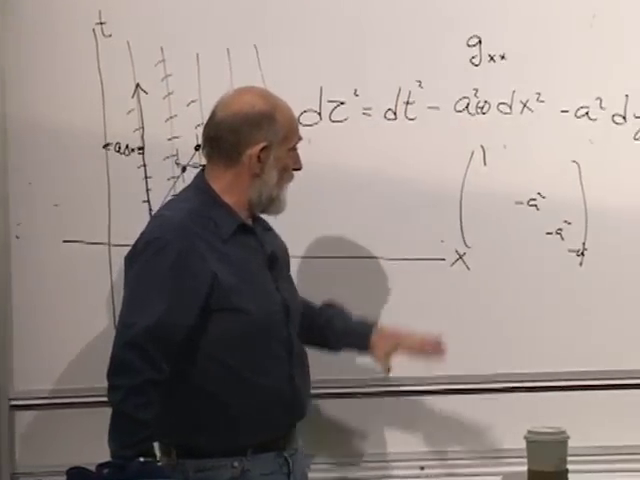
\includegraphics[width=0.82\textwidth]{lecture_01_figure_02.png}\caption{Líneas de universo comóviles en un universo unidimensional en expansión, junto con el intervalo de espacio-tiempo correspondiente.}\end{figure}

En tres dimensiones espaciales, el mismo esquema da la extensión, con las debidas precauciones\footnote{La pizarra está parcialmente oculta alrededor de 00:56:38--00:58:51. Esta forma tridimensional recoge la extensión oral de una a tres dimensiones espaciales, junto con el patrón diagonal visible en la pizarra.}
\begin{equation}
d\tau^2=dt^2-a^2(t)\bigl(dx^2+dy^2+dz^2\bigr),
\end{equation}
con métrica diagonal
\begin{equation}
g_{\mu\nu}=\mathrm{diag}\bigl(1,-a^2,-a^2,-a^2\bigr).
\end{equation}
Los términos no diagonales se anulan:
\begin{equation}
g_{tx}=g_{ty}=g_{tz}=0.
\end{equation}

La homogeneidad significa que los coeficientes de la métrica pueden depender del tiempo, pero no de la posición espacial. La isotropía significa que las tres direcciones espaciales intervienen del mismo modo.

\begin{classroomqa}\audiencequestion{¿No se supone que debemos interpretar \(dx\) como una distancia?}\lecturetimestamp{01:01:18}\lecturerresponse{No. \(dx\) no es la distancia. \(a\,dx\) es la distancia. \(dx\) es solo un intervalo entre etiquetas. Una forma útil de entenderlo es imaginar que, en cierto momento, alguien traza una cuadrícula de coordenadas a través de las galaxias y luego exige que la cuadrícula las siga. La separación entre coordenadas permanece fija por construcción, mientras que la distancia física cambia. Se podrían incluir las unidades de distancia en \(x\) en vez de en \(a\); eso es una convención. Lo que importa es el producto \(a\,dx\).}\end{classroomqa}

\begin{classroomqa}\audiencequestion{El coeficiente métrico de \(dt^2\) es igual a \(1\). ¿Eso también es solo una convención?}\lecturetimestamp{01:03:24}\lecturerresponse{Sí. Eso, por sí solo, no tiene contenido físico. Si el coeficiente dependiera solo del tiempo, se podría cambiar la variable temporal para que pasara a ser simplemente \(dt^2\). Del mismo modo, se pueden elegir unidades en las que \(c=1\). Lo que aquí no es una convención es que el coeficiente no dependa de la posición, aunque sí pueda depender del tiempo.}\end{classroomqa}

\begin{classroomqa}\audiencequestion{Si se introduce esto en las ecuaciones de campo de Einstein, ¿qué se obtiene para el tensor de energía-momento?}\lecturetimestamp{01:05:59}\lecturerresponse{Ese es el tipo de pregunta que viene a continuación, pero pertenece a la dinámica, no al tema que estamos tratando ahora. Se puede introducir esta métrica en las ecuaciones de Einstein y preguntar qué distribución de energía-momento haría que fuera una solución. Eso es muy importante, pero por el momento nos ocupamos de la geometría, no de la dinámica.}\end{classroomqa}

\section{Lo que oculta el horizonte}

El universo a gran escala se considera homogéneo e isótropo solo como aproximación. Desde luego, no es homogéneo a la escala de las estrellas, los planetas ni siquiera las galaxias individuales. Tampoco es exactamente isótropo en todas las observaciones locales.

Un campo de cultivo ilustra bien la dependencia de la escala. A cierta escala parece regular; a una escala mucho menor, evidentemente no lo es; y a una escala mayor que el campo entero, deja de parecer homogéneo otra vez. En cosmología ocurre lo mismo. Tras promediar sobre muchas galaxias, la distribución a gran escala parece aproximadamente uniforme. A escalas suficientemente pequeñas, no lo es.

El universo es más grande que la parte que podemos ver, y más grande que la parte que podremos ver jamás. En las escalas que realmente podemos explorar, es isótropo y homogéneo, salvo por variaciones locales. Más allá de eso, no hay ninguna garantía observacional directa.

\begin{classroomqa}\audiencequestion{Dijo que nunca llegaremos a saberlo directamente. ¿Eso implica que quizá haya una forma indirecta de averiguarlo?}\lecturetimestamp{01:10:34}\lecturerresponse{Quizá. Hoy en día, la mayoría piensa que, a escalas suficientemente grandes, el universo no es homogéneo, y yo apuesto por lo mismo. Pero es una apuesta que nunca podré ganar ni perder, porque, por razones fundamentales, no podremos ver mucho más allá de lo que vemos ahora. Eso se debe a la existencia de un horizonte.}\end{classroomqa}

\begin{classroomqa}\audiencequestion{¿No se podría usar la gravedad para buscar masas más allá de lo que podemos ver?}\lecturetimestamp{01:11:53}\lecturerresponse{No. Una masa distante puede simplemente hacernos caer en caída libre. Estamos en una habitación cerrada, dentro del campo gravitatorio del Sol y orbitándolo, pero, si no podemos mirar al exterior, no hay una manera fácil de saber que el Sol está ahí. Solo las fuerzas de marea lo revelarían y, si la fuente estuviera lo bastante lejos, esos efectos de marea podrían ser demasiado pequeños para detectarlos.}\end{classroomqa}

Por tanto, el horizonte es una barrera definitiva para el conocimiento directo. Incluso afirma, con prácticamente total certeza, que el volumen del universo es al menos mil veces mayor que el de la región que jamás podremos ver, y deja para más adelante la explicación de esa afirmación.

\section{Finito y sin frontera}

Pasemos ahora a las geometrías cerradas. La línea infinita es abierta e ilimitada. Un segmento de recta es acotado, en el sentido de que tiene una extensión finita. Acotado no significa que tenga una frontera, sino que su extensión es finita.

Un cubo con paredes no sirve. Viola la homogeneidad, porque alguien cerca de una pared no es equivalente a alguien lejos de ella, y viola la isotropía, porque incluso quien está en el centro ve cosas distintas en distintas direcciones.

El interior de un círculo o de una esfera tampoco sirve. Alguien en el centro ve lo mismo en todas las direcciones, pero esa simetría solo corresponde a un punto especial. Si se aleja del centro, la pared está cerca en una dirección y lejos en otra. Por tanto, para observadores genéricos, el espacio no es ni homogéneo ni isótropo.

La hipótesis de trabajo a escalas muy grandes es que el universo es homogéneo e isótropo. Este es el principio cosmológico. Es útil, pero nada impide que se revise.

\begin{classroomqa}\audiencequestion{¿La isotropía en todas partes implica homogeneidad?}\lecturetimestamp{01:18:57}\lecturerresponse{Sí. Si todos los observadores ven lo mismo en todas las direcciones, eso implica homogeneidad. Pero la implicación inversa no se cumple. La homogeneidad por sí sola no implica isotropía. Un universo puede ser homogéneo y, aun así, tener una dirección privilegiada; por ejemplo, si estuviera lleno de flechas que apuntaran todas en la misma dirección.}\end{classroomqa}

El modelo acotado adecuado es la superficie de una esfera sin rasgos distintivos. Una criatura bidimensional confinada a esa superficie encuentra cada lugar localmente igual a cualquier otro y cada dirección igual a cualquier otra, aunque el mundo sea finito. Eso es ser finito y carecer de frontera.

\section{Un universo unidimensional cerrado en forma de círculo}

Para simplificar el álgebra, reduzcamos el ejemplo de la esfera a una dimensión espacial: la vida en un círculo. En una dimensión, isotropía significa que izquierda y derecha son equivalentes. Un círculo tiene exactamente esa propiedad. Elijamos un punto y llamémoslo \(\theta=0\). A todos los demás puntos se les asigna una coordenada angular \(\theta\), medida en radianes. Un punto justo a un lado del origen puede describirse con un ángulo negativo pequeño o con uno apenas menor que \(2\pi\). Esa periodicidad forma parte de la geometría.

Los habitantes del círculo tienen acceso a la circunferencia, no a un radio ni a un centro externos. Pueden medir la distancia total alrededor recorriendo el círculo hasta regresar al mismo punto. Si se dibuja el círculo en un plano que lo contiene, también se puede introducir una cantidad análoga al radio, pero eso pertenece a la representación mediante una inmersión, no a la geometría intrínseca que ellos miden.

El dibujo de la pizarra es útil aquí porque muestra en un mismo esquema las etiquetas angulares y la circunferencia total.
\begin{figure}[H]\centering
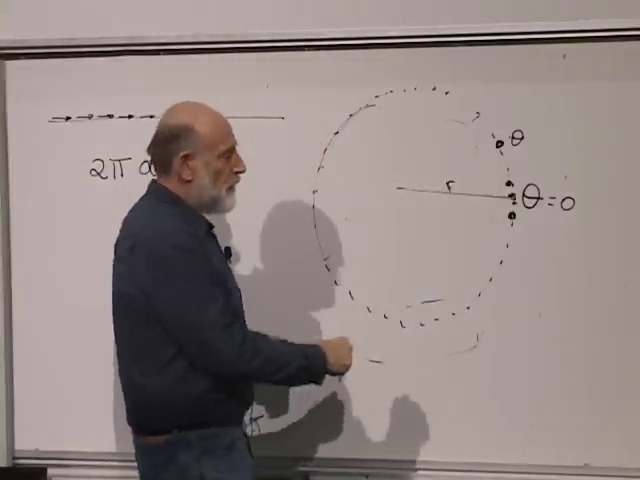
\includegraphics[width=0.82\textwidth]{lecture_01_figure_03.png}\caption{Descripción angular de un universo unidimensional cerrado, con circunferencia total \(2\pi a\).}\end{figure}

Una convención práctica es\footnote{En torno a 01:26:40--01:29:20, la notación cambia brevemente entre tomar la circunferencia completa como factor de escala y escribirla como \(2\pi a\). Aquí se usa la convención posterior, porque es la que se incorpora a la fórmula de longitud de arco.}
\begin{equation}
L=2\pi a,
\end{equation}
donde \(L\) es la circunferencia total.

Para una pequeña separación angular \(\Delta\theta\), la distancia física es
\begin{equation}
d=a\,\Delta\theta.
\end{equation}
Al pasar a diferenciales, se obtiene
\begin{equation}
ds=a\,d\theta,
\end{equation}
y, por tanto,
\begin{equation}
ds^2=a^2\,d\theta^2.
\end{equation}
Esta es la métrica local del círculo.

Si \(a\) depende del tiempo, el universo unidimensional cerrado se expande o se contrae. Para un par fijo de galaxias,
\begin{equation}
d(t)=a(t)\,\Delta\theta,
\end{equation}
por lo que
\begin{equation}
\dot d=\dot a\,\Delta\theta
      =\frac{\dot a}{a}\,d.
\end{equation}
La ley de Hubble también se cumple aquí, al menos para pares que no estén tan alejados que resulte ambiguo cuál de los dos caminos alrededor del círculo se toma.

La métrica del espacio-tiempo pasa a ser
\begin{equation}
d\tau^2=dt^2-a^2(t)\,d\theta^2.
\end{equation}
Si \(a\) es constante, la representación del espacio-tiempo es un cilindro. Si \(a\propto t\), es un cono. Si \(a(t)\) cambia de manera más irregular, la representación adquiere forma de vaso.

Si seguimos el dibujo hacia atrás en el tiempo, las galaxias se acercan cada vez más. Si hubiera \(360\) galaxias alrededor del círculo, estarían bien separadas en épocas tardías, muy juntas en épocas anteriores y aún más juntas antes. Al final dejarían de ser galaxias separadas y, en épocas todavía anteriores, ni siquiera serían átomos separados. Pero sigue sin haber ningún punto especial en el espacio.

Esta es la respuesta más clara, dentro del modelo, a la pregunta de dónde ocurrió el Big Bang. Cuando \(a(t)\to 0\), todas las separaciones \(a(t)\,\Delta\theta\) se anulan. El universo entero se contrae en todas partes a la vez. Las galaxias no salen disparadas desde un lugar privilegiado hacia un espacio exterior. Lo que cambia de escala es la propia geometría. En ese sentido, la respuesta es: en todas partes.

\begin{classroomqa}\audiencequestion{Dijo que el espacio-tiempo está curvado. ¿Estaría curvado si tuviera forma de cilindro?}\lecturetimestamp{01:38:04}\lecturerresponse{No. Si tuviera forma de cilindro, no estaría curvado. Ese es el caso en que \(a\) es constante en el tiempo. Solo parece curvado porque se dibuja en un espacio de más dimensiones. Si se corta y se abre, se puede extender plano sin estirarlo.}\end{classroomqa}

A partir de ahí, la discusión pasa al cono. Si \(a\propto t\), la representación del espacio-tiempo es un cono. Salvo en su vértice, el cono también es plano en el mismo sentido intrínseco: se puede abrir para formar un plano. El vértice es distinto. Es una singularidad cónica.

El siguiente paso es estudiar la geometría del universo esférico y, después, la dinámica que determina cómo \(a(t)\) crece o se contrae.

\chapter{Cosmología newtoniana y ecuación de Friedmann}

La última vez hablamos de la métrica del espacio. La siguiente pregunta es sobre la dinámica: ¿cómo cambia el factor de escala con el tiempo? Primero veremos un poco de geometría y después, cosmología newtoniana. Todavía no deduciremos la ecuación de Friedmann a partir de la relatividad general; la deduciremos de las ecuaciones de Newton.

\section{Homogeneidad, isotropía y una métrica dependiente del tiempo}

La homogeneidad y la isotropía son los supuestos de partida. Si el universo es homogéneo e isótropo y cambia con el tiempo, la ley de Hubble siempre se cumple. En cualquier instante, la velocidad de recesión es proporcional a la distancia,
\begin{equation}
v = H(t)\,d.
\end{equation}
La proporcionalidad es lineal. Lo que permanece constante no es el tiempo, sino el espacio: en un instante dado, el mismo factor de proporcionalidad se aplica en todas partes.

\begin{classroomqa}
\audiencequestion{¿Eso significa que son linealmente proporcionales?}\lecturetimestamp{00:02:06}
\lecturerresponse{Sí. En un instante dado, la velocidad de recesión es linealmente proporcional a la distancia. El factor de proporcionalidad es la constante de Hubble. En general, depende del tiempo, pero no varía de un punto a otro del espacio.}
\end{classroomqa}

Por eso es peligrosa la expresión ``constante de Hubble''. Es constante con respecto a la posición en el espacio, pero no con respecto al tiempo.

A continuación surge una pregunta natural. Si el espacio se expande, ¿por qué no se expanden también las reglas métricas? La respuesta es que las fuerzas que mantienen unidas las reglas métricas son muchísimo más intensas que cualquier efecto asociado con la expansión cosmológica a escala atómica. Los objetos ligados permanecen ligados. Lo que se expande es la distancia entre cosas suficientemente separadas, como las galaxias que están tan lejos unas de otras que no se mantienen fuertemente unidas.

\begin{classroomqa}
\audiencequestion{¿Hay algún problema con el hecho de que las reglas de medición también se estén expandiendo?}\lecturetimestamp{00:04:00}
\lecturerresponse{No. Las reglas de medición no se expanden; se expanden las coordenadas. Las fuerzas que mantienen unidas las reglas métricas son mucho más intensas que los efectos de la expansión, por lo que los objetos ligados ordinarios no se expanden con el fondo. Las galaxias suficientemente alejadas sí se separan, pero las reglas métricas no.}
\end{classroomqa}

Incluso se puede imaginar un efecto repulsivo adicional, muy pequeño, entre los átomos. Aun así, no bastaría para romper una regla. Solo desplazaría un poco la separación de equilibrio, como una pequeña fuerza adicional desplaza la posición de equilibrio de un resorte rígido.

\begin{classroomqa}
\audiencequestion{Pero no se puede modelar como una fuerza entre puntos, ¿es correcto? Porque, de lo contrario, habría una aceleración.}\lecturetimestamp{00:05:29}
\lecturerresponse{Se puede imaginar una pequeña fuerza adicional entre los átomos, pero, si es diminuta en comparación con las fuerzas de enlace, solo desplaza ligeramente la posición de equilibrio. La expansión, por sí sola, no genera una ley de fuerzas ordinaria. Algunos tipos de expansión sí se pueden modelar en términos de una fuerza, concretamente la expansión acelerada, pero esa es una cuestión que veremos más adelante.}
\end{classroomqa}

Así pues, las coordenadas útiles son las que están inmersas en la distribución de materia en expansión. Las galaxias que no tienen movimiento peculiar adicional conservan los mismos valores de coordenadas. Lo que cambia con el tiempo es la relación entre la separación en coordenadas y la distancia física medida en metros. Esa relación queda expresada por el factor de escala \(a(t)\).

Para un espacio plano, la métrica espacial se puede escribir como
\begin{equation}
ds^2 = a(t)^2\left(dx^2+dy^2+dz^2\right).
\end{equation}
Aquí, \(a\) es la distancia real, medida en metros, entre puntos vecinos separados por una unidad de distancia en coordenadas. Si el universo se expande, \(a\) depende del tiempo.

Para pasar al espacio-tiempo, partamos de la forma relativista especial
\begin{equation}
d\tau^2 = dt^2 - ds^2,
\end{equation}
y sustituyamos la métrica espacial. Se obtiene
\begin{equation}
d\tau^2 = dt^2 - a(t)^2\left(dx^2+dy^2+dz^2\right).
\end{equation}
Los coeficientes no dependen de la posición en el espacio, sino únicamente del tiempo. En el lenguaje de las métricas, eso es lo que significa homogeneidad. La métrica diagonal tiene la forma
\begin{equation}
g_{\mu\nu}=\mathrm{diag}\!\left(1,-a(t)^2,-a(t)^2,-a(t)^2\right).
\end{equation}
\editorialnote{La matriz diagonal completa que se muestra aquí se basa en la descripción oral del tensor métrico que aparece entre 00:14:33. El encuadre de la pizarra permite ver claramente el elemento de línea, pero no una matriz que se pueda leer por completo.}

No hay términos no diagonales: ni \(dx\,dy\), ni \(dx\,dt\), ni otros términos mixtos. La métrica es casi tan sencilla como la del espacio-tiempo plano. Su peculiaridad es que la relación entre la medida espacial y el tiempo depende, a su vez, del tiempo.

\begin{figure}
\centering
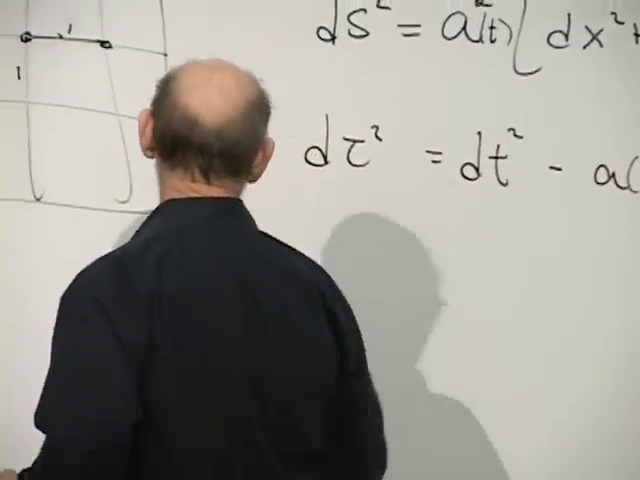
\includegraphics[width=0.62\textwidth]{lecture_02_figure_02.png}
\caption{Esquema de una retícula comóvil y del intervalo espacio-temporal con un factor de escala dependiente del tiempo.}
\end{figure}

La figura ilustra la idea. Alice y Bob permanecen separados por una unidad en las coordenadas comóviles, pero esa unidad de coordenadas representa cada vez más metros a medida que pasa el tiempo. Si \(a(t)\) hubiera sido cero en algún momento del pasado, todas las separaciones físicas habrían sido nulas: todo habría quedado aplastado junto. Por eso \(a\to 0\) corresponde a una densidad infinita. A medida que \(a\) crece, el universo se vuelve cada vez más difuso.

Esta forma de la métrica no es válida en todos los sistemas de referencia. Es la forma que tiene en el sistema que se mueve con las galaxias.

\begin{classroomqa}
\audiencequestion{En esa ecuación, la pequeña \(t\), \(a(t)\), ¿a qué tiempo \(t\) corresponde?}\lecturetimestamp{00:19:19}
\lecturerresponse{Es el tiempo que miden los relojes que se mueven con las galaxias. Imaginemos relojes idénticos, fabricados en la misma fábrica de relojes cósmicos y transportados por las galaxias. En este sistema de referencia, la variable temporal es exactamente lo que miden esos relojes. A lo largo de la línea de universo de una galaxia, el tiempo propio coincide con este tiempo coordenado.}
\end{classroomqa}

En efecto, a lo largo de la línea de universo de una galaxia comóvil,
\begin{equation}
dx=dy=dz=0,
\end{equation}
por lo que
\begin{equation}
d\tau^2 = dt^2,
\end{equation}
y, por tanto,
\begin{equation}
dt=d\tau.
\end{equation}

\begin{classroomqa}
\audiencequestion{¿Hay transformaciones que dejen invariante esta forma de la métrica?}\lecturetimestamp{00:23:08}
\lecturerresponse{Las rotaciones sí, porque \(dx^2+dy^2+dz^2\) es invariante bajo rotaciones. Las transformaciones de Lorentz, en cambio, no conservan esta forma. La propia materia selecciona el sistema de referencia que se mueve con las galaxias; en cualquier otro sistema, el universo no se vería isótropo.}
\end{classroomqa}

\section{Un proyectil en un campo gravitatorio}

Antes de aplicar las leyes de Newton al universo entero, conviene volver a un problema más sencillo: una masa grande \(M\), una masa mucho menor \(m\) y un impulso inicial hacia fuera. Después del impulso, la masa pequeña simplemente se mueve en el campo gravitatorio y hace lo que dictan las leyes de Newton.

Para la discusión cosmológica, lo importante no es resolver la órbita completa, sino la conservación de la energía. La energía cinética es
\begin{equation}
\frac{1}{2}mv^2.
\end{equation}

\begin{figure}
\centering
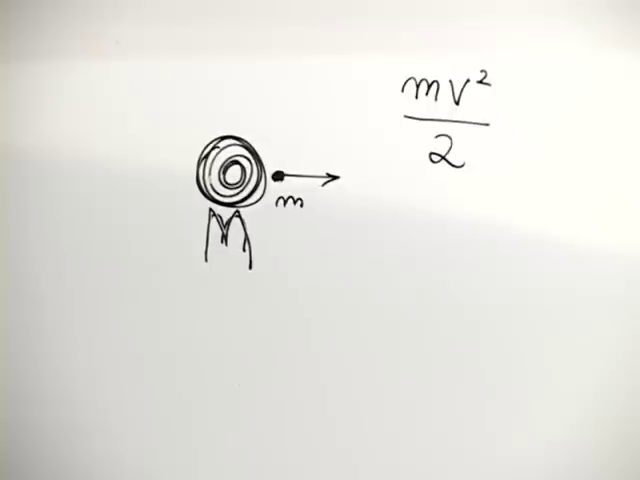
\includegraphics[width=0.42\textwidth]{lecture_02_figure_03.png}
\caption{Masa de prueba que se aleja y término de energía cinética \(\frac{1}{2}mv^2\).}
\end{figure}

La energía potencial gravitatoria contiene el producto de las masas, la constante de Newton y una potencia de la distancia en el denominador. En la expresión escrita en la pizarra, los factores aparecen en el orden \(mMG/D\), así que conviene conservar aquí ese orden:
\begin{equation}
-\frac{mMG}{D}.
\end{equation}
Por tanto, la energía total es
\begin{equation}
\frac{1}{2}mv^2-\frac{mMG}{D}.
\end{equation}
La conservación de la energía solo afirma que esta cantidad no cambia con el tiempo para la partícula en cuestión. Distintas partículas pueden tener energías distintas.

\begin{figure}
\centering
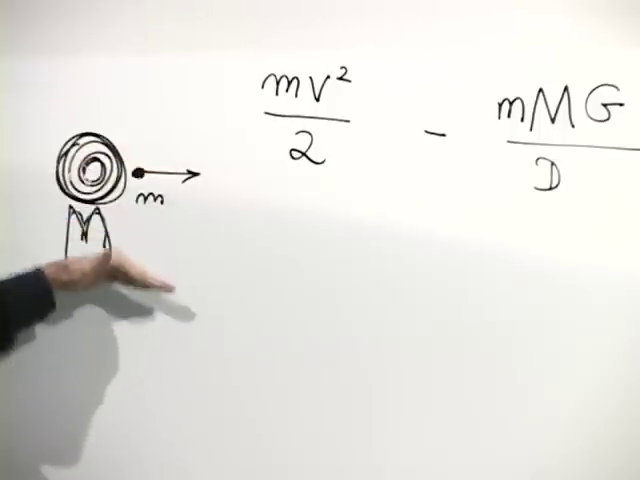
\includegraphics[width=0.62\textwidth]{lecture_02_figure_04.png}
\caption{Energía newtoniana total de una masa de prueba en movimiento radial: término cinético menos potencial gravitatorio.}
\end{figure}

El signo negativo es importante. La energía potencial gravitatoria es negativa porque la gravedad es atractiva. Al acercar la partícula, aumenta la magnitud de la energía potencial negativa. Al alejarla, la energía potencial se vuelve menos negativa.

\begin{classroomqa}
\audiencequestion{¿La energía potencial aumenta con la distancia en vez de disminuir?}\lecturetimestamp{00:34:13}
\lecturerresponse{Sí. Dejemos de lado las constantes y observemos las gráficas de \(1/D\) y \(-1/D\). La fuerza impulsa el movimiento hacia valores menores de energía potencial. Por tanto, una fuerza atractiva corresponde a la curva invertida, \(-1/D\): la energía potencial aumenta con la distancia y se hace más negativa a medida que la partícula se acerca.}
\end{classroomqa}

\begin{figure}
\centering
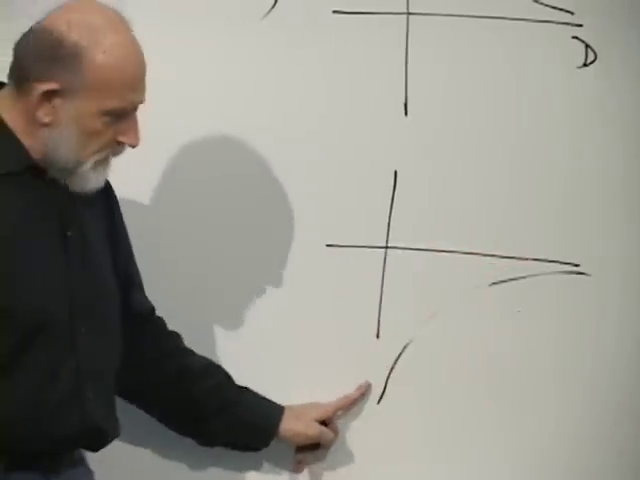
\includegraphics[width=0.46\textwidth]{lecture_02_figure_05.png}
\caption{Comparación cualitativa de \(1/D\) y \(-1/D\) para determinar el signo de la energía potencial gravitatoria.}
\end{figure}

\section{Velocidad de escape}

Clasifiquemos ahora las posibilidades. La energía puede ser positiva, negativa o nula. Esos son los únicos tres casos.

\begin{itemize}
\item Si la energía es negativa, la partícula está ligada. Si se la lanza hacia arriba con una velocidad demasiado pequeña, asciende, pierde velocidad, se detiene y vuelve a caer.
\item Si la energía es positiva, la partícula escapa. Al principio, la gravedad la desacelera, pero no lo suficiente como para detenerla, y al final se aleja con una velocidad de salida asintótica distinta de cero.
\item Si la energía es exactamente nula, la partícula tiene la velocidad de escape. Es el caso límite entre escapar y no hacerlo.
\end{itemize}

Si la velocidad inicial es suficientemente pequeña, el término potencial domina desde el principio y la energía es negativa.

\begin{figure}
\centering
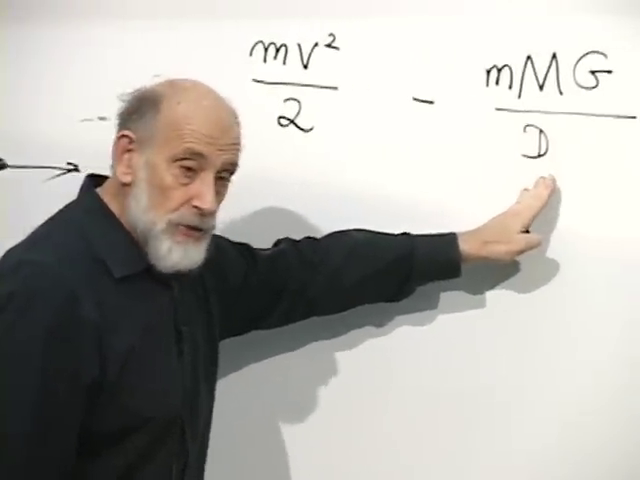
\includegraphics[width=0.62\textwidth]{lecture_02_figure_06.png}
\caption{A baja velocidad inicial hacia fuera, el término potencial negativo domina la energía total.}
\end{figure}

En el caso de energía nula, la distancia sigue aumentando, pero la rapidez sigue disminuyendo. La partícula no puede detenerse en ningún tiempo finito. Si lo hiciera, volvería a caer. Así pues, la distancia no está acotada, mientras que la velocidad tiende a cero.

Esta es la analogía directa que importa para la cosmología. El universo puede comportarse de la misma manera. Si el flujo de Hubble inicial hacia fuera es suficientemente grande, todo escapa de todo lo demás. Si es demasiado pequeño, la gravedad prevalece y se produce un gran colapso. También existe el caso límite, exactamente análogo a la velocidad de escape.

\section{Teorema de Newton}

La reducción cosmológica funciona gracias al teorema de Newton para la ley del inverso del cuadrado.

Si la materia está distribuida con simetría esférica alrededor de un centro, la fuerza gravitatoria sobre una partícula exterior a la distribución es exactamente la misma que si toda la masa estuviera concentrada en el centro. Pero el teorema es aún más potente. Si la partícula está dentro de la distribución, solo contribuye la masa situada a radios menores. La masa situada a radios mayores no produce fuerza neta.

La versión más clara del teorema es la de una cáscara esférica delgada. Una cáscara esférica perfecta no ejerce fuerza gravitatoria sobre ninguna partícula situada en su interior, ni siquiera si está fuera del centro. A primera vista sorprende, pero es cierto para la ley \(1/r^2\).

\begin{classroomqa}
\audiencequestion{En el ejemplo que acaba de dar, ¿no debería sorprendernos un poco que la fuerza parezca discontinua cuando la partícula cruza el límite?}\lecturetimestamp{00:48:19}
\lecturerresponse{Sí. Resulta sorprendente en el caso de una cáscara ideal infinitamente delgada, y es una propiedad exclusiva de la ley de fuerza \(1/r^2\). Una cáscara real tiene grosor, así que la variación se suaviza; pero la afirmación tajante para una cáscara ideal es precisamente la notable propiedad del teorema de Newton.}
\end{classroomqa}

Una imagen ayuda a hacer plausible el teorema. Sustituyamos una masa puntual por una fuente puntual de agua. En tres dimensiones, el flujo hacia fuera disminuye como \(1/r^2\). Dispongamos fuentes de ese tipo de manera continua por toda una cáscara esférica. Fuera de la cáscara, el flujo es exactamente igual que si todo estuviera concentrado en el centro. Dentro de ella no puede haber flujo neto, porque no hay ninguna fuente en el centro. Esa misma estructura es la que sustenta el teorema gravitatorio.

La idea aquí no es volver a demostrar el teorema, sino utilizarlo.

\section{Un universo homogéneo como problema de dos cuerpos}

Volvamos ahora a la cosmología. Tomemos una pequeña región del universo llena de un gas uniforme de galaxias. Si se quiere, uno puede situarse en el centro. Es solo una comodidad. Cualquiera puede decir que está en el centro, y debe resultar la misma ecuación.

Elijamos una galaxia sobre el eje \(x\), en la coordenada comóvil \(x\). Como el universo es isótropo, da igual qué eje escojamos. Tracemos una esfera centrada en \(x=0\) que pase por esa galaxia. Según el teorema de Newton, la fuerza sobre la galaxia es exactamente la misma que si toda la masa dentro de la esfera estuviera concentrada en el centro; todo lo que queda fuera no contribuye.

La esfera se expande junto con las galaxias. Siempre contiene las mismas galaxias y, por tanto, la misma masa total, aunque su radio físico cambie con el tiempo.

Por tanto, el movimiento de esa galaxia obedece exactamente al mismo tipo de ecuación de la energía que el proyectil:
\begin{equation}
\frac{1}{2}mv^2-\frac{mMG}{D}=\text{constant}.
\end{equation}
Aquí, \(M\) representa ahora la masa dentro de la esfera en expansión, no la masa central del ejemplo introductorio. Luego se simplifica el álgebra multiplicando por \(2\) y dividiendo por \(m\). Como una constante dividida por \(m\) sigue siendo simplemente una constante, podemos escribir
\begin{equation}
v^2-\frac{2MG}{D}=\text{constant}.
\end{equation}
De nuevo, ``constante'' significa constante en el tiempo para esa galaxia concreta.

Relacionemos ahora esto con el factor de escala. La distancia física a la galaxia es
\begin{equation}
D=ax,
\end{equation}
porque \(x\) es una coordenada comóvil fija. Su velocidad es
\begin{equation}
v=\dot D=\dot a\,x.
\end{equation}

La masa dentro de la esfera es la densidad multiplicada por el volumen. Si \(\rho\) es la densidad de masa, entonces
\begin{equation}
M=\frac{4\pi}{3}\rho D^3=\frac{4\pi}{3}\rho a^3x^3.
\end{equation}
Al sustituirlo en la ecuación de la energía se obtiene
\begin{equation}
\dot a^2x^2-\frac{2G}{ax}\left(\frac{4\pi}{3}\rho a^3x^3\right)=\text{constant},
\end{equation}
o bien
\begin{equation}
\dot a^2x^2-\frac{8\pi G}{3}\rho a^2x^2=\text{constant}.
\end{equation}

Los dos términos del lado izquierdo son proporcionales a \(x^2\). Todo lo demás en ese lado es igual en todas partes. Por lo tanto, el lado derecho también debe ser proporcional a \(x^2\). Esto no contradice que lo llamemos constante. Significa que es constante con respecto al tiempo para cada \(x\) fijo, pero aun así puede escalar con \(x^2\) de una galaxia a otra. Tiene sentido: las galaxias más lejanas se mueven más rápido.

Dividamos, pues, por el factor común \(x^2\). La constante restante ya es independiente tanto del tiempo como del espacio. Escribámosla de la forma históricamente convencional \(-k\):
\begin{equation}
\dot a^2-\frac{8\pi G}{3}\rho a^2=-k.
\end{equation}
Después de dividir por \(a^2\),
\begin{equation}
\left(\frac{\dot a}{a}\right)^2=\frac{8\pi G}{3}\rho-\frac{k}{a^2}.
\end{equation}

Esta es la famosa ecuación de Friedmann-Robertson-Walker, aunque en la clase también se señala que, en realidad, es la ecuación de Friedmann. La convención de signos es histórica. Escribir \(-k\) no significa que \(k\) tenga que ser positivo. \(k\) puede ser positivo, negativo o nulo. En unidades en las que la velocidad de la luz es igual a \(1\), \(k\) es adimensional.

\section{Densidad y ecuación para un universo dominado por la materia}

La siguiente pregunta es inmediata: ¿qué es \(\rho\)? No es constante. A medida que el universo se expande, la densidad disminuye.

Para expresar esa dependencia, tomemos un cubo unidad en el espacio de coordenadas: una unidad por lado en \(x\), \(y\) y \(z\). Las mismas galaxias permanecen dentro de ese cubo en todo momento porque el cubo se expande junto con las coordenadas. Así que la masa dentro de ese cubo de coordenadas permanece fija.

\editorialnote{En varias etapas, la clase reutiliza el símbolo \(M\). Aquí se usa \(M_{\Box}\) únicamente para distinguir la masa contenida en un cubo unidad de coordenadas de la masa central y la masa encerrada en la esfera anteriores.}

La longitud física de cada lado del cubo es \(a\), así que su volumen físico es \(a^3\). Por tanto,
\begin{equation}
\rho=\frac{M_{\Box}}{a^3}.
\end{equation}
Este es el caso dominado por la materia: el lado derecho contiene únicamente la densidad de la materia ordinaria no relativista.

\begin{classroomqa}
\audiencequestion{Según esa ecuación, la constante de Hubble es función de \(\rho\). Así que no es constante.}\lecturetimestamp{01:19:21}
\lecturerresponse{Exactamente. La constante de Hubble no es constante. Depende de la densidad, y la densidad cambia con el tiempo. Incluso se bromea en la clase con que el examen final podría consistir en una sola pregunta: ¿Es constante la constante de Hubble?}
\end{classroomqa}

Al sustituir \(\rho=M_{\Box}/a^3\) en la ecuación de Friedmann se obtiene
\begin{equation}
\left(\frac{\dot a}{a}\right)^2=\frac{8\pi G M_{\Box}}{3a^3}-\frac{k}{a^2}.
\end{equation}

En este punto quedan claras las elecciones arbitrarias. Se necesitan la masa contenida en un cubo unidad de coordenadas y el valor de \(k\). Los tres signos posibles de \(k\) corresponden a los tres casos de energía del problema del proyectil.

\begin{itemize}
\item Si \(-k>0\), la energía supera efectivamente la velocidad de escape y el universo se expande para siempre.
\item Si \(-k<0\), la gravedad acaba prevaleciendo y el universo vuelve a colapsar.
\item Si \(k=0\), el universo está exactamente en el caso de la velocidad de escape.
\end{itemize}

\begin{classroomqa}
\audiencequestion{¿Es \(k=0\)? Entonces, ¿la velocidad relativa entre dos galaxias se aproxima a cero?}\lecturetimestamp{01:21:12}
\lecturerresponse{Sí. En el caso crítico, la velocidad se aproxima a cero, pero la distancia sigue sin estar acotada. Las galaxias siguen separándose, aunque cada vez más despacio. Si de hecho se detuvieran en algún tiempo finito, volverían a caer.}
\end{classroomqa}

\section{El caso crítico \(k=0\)}

Elijamos ahora el caso más sencillo, \(k=0\). Es el caso exacto de la velocidad de escape y resulta más sencillo únicamente porque las matemáticas son más simples. La ecuación queda
\begin{equation}
\left(\frac{\dot a}{a}\right)^2=\frac{8\pi G M_{\Box}}{3a^3}.
\end{equation}

El lado derecho siempre es positivo y nunca se anula. Por tanto, \(\dot a/a\) no puede pasar por cero. En este caso, el universo no puede invertir el sentido de su evolución. O bien siempre se está expandiendo, o bien siempre se está contrayendo. Tomemos la rama de expansión.

Probemos ahora con una ley potencial,
\begin{equation}
a(t)=ct^p.
\end{equation}
Entonces
\begin{equation}
\dot a = cp\,t^{p-1},
\end{equation}
y, por tanto,
\begin{equation}
\frac{\dot a}{a}=\frac{p}{t}.
\end{equation}
Al sustituir en la ecuación diferencial se obtiene
\begin{equation}
\frac{p^2}{t^2}=\frac{8\pi G M_{\Box}}{3c^3t^{3p}}.
\end{equation}
Para que coincidan las potencias de \(t\), debe cumplirse
\begin{equation}
3p=2.
\end{equation}
Así que
\begin{equation}
p=\frac{2}{3}.
\end{equation}
Entonces, las constantes deben satisfacer
\begin{equation}
\frac{4}{9}=\frac{8\pi G M_{\Box}}{3c^3},
\end{equation}
de donde
\begin{equation}
c^3=6\pi G M_{\Box}.
\end{equation}
Por tanto,
\begin{equation}
a(t)=\left(6\pi G M_{\Box}\right)^{1/3}t^{2/3}.
\end{equation}

Todavía puede haber un desplazamiento aditivo en el tiempo. Se absorbe sustituyendo \(t\) por \(t-t_0\). Una vez que se elige el origen temporal de modo que \(a=0\) en \(t=0\), esa constante restante desaparece.

Así pues, el universo se expande según la potencia dos tercios del tiempo,
\begin{equation}
a(t)\propto t^{2/3}.
\end{equation}
No se expande linealmente con el tiempo. El crecimiento lineal sería análogo a un movimiento sin aceleración. En este caso, la expansión se desacelera.

Si prolongamos la fórmula hacia atrás hasta \(t=0\), el factor de escala tiende a cero y la densidad diverge. Decir \(a=0\) es una afirmación extrema. No sabemos qué ocurre con la materia cuando alcanza densidades demasiado altas. Lo esencial es que, en una etapa temprana, todo estaba tan apretado que los átomos, los núcleos y los quarks se encontraban juntos en un estado extraordinariamente denso.

\section{La constante de Hubble y la edad del universo}

En el modelo crítico,
\begin{equation}
H(t)=\frac{\dot a}{a}=\frac{2}{3t}.
\end{equation}
Así que la constante de Hubble es aproximadamente el inverso de la edad del universo,
\begin{equation}
t=\frac{2}{3H}.
\end{equation}
Este es uno de los principales resultados del cálculo. Si se mide la constante de Hubble hoy, se obtiene una estimación de la edad del universo, al menos hasta el punto en que el modelo newtoniano deja de tener sentido.

La edad que se cita es de aproximadamente \(13\) a \(14\) mil millones de años. El texto también señala que \(k=0\) concuerda muy bien con las observaciones: con el nivel de precisión indicado, no se conoce ninguna desviación significativa de \(k=0\).

\begin{classroomqa}
\audiencequestion{Me confunde un poco qué son \(M\) y \(a\).}\lecturetimestamp{01:39:16}
\lecturerresponse{Ambas cantidades dependen de cómo se elija la retícula. Si se cambia la caja de referencia, cambia la cantidad de materia que contiene y también el valor numérico del factor de escala. La magnitud física es la densidad, \(M/a^3\), o, de manera equivalente, combinaciones como \(a/M^{1/3}\), que no dependen de cómo se elija la retícula. En la solución con \(k=0\), la constante desconocida que multiplica a \(t^{2/3}\) se cancela en \(\dot a/a\), de modo que la relación de edad \(t=2/3H\) no depende de la masa de la caja de referencia.}
\end{classroomqa}

La cancelación se ve de inmediato en la solución. Si
\begin{equation}
a(t)=Ct^{2/3},
\end{equation}
entonces
\begin{equation}
\dot a=\frac{2}{3}Ct^{-1/3},
\end{equation}
y, por tanto,
\begin{equation}
\frac{\dot a}{a}=\frac{2}{3t}.
\end{equation}
La constante \(C\) desaparece por completo.

\section{Por qué funciona la derivación newtoniana}

Hacia el final, la pregunta pasa a ser: ¿por qué debería concordar tan bien la derivación newtoniana con la relativista?

\begin{classroomqa}
\audiencequestion{Todo esto parece depender del supuesto de que el universo es abierto.}\lecturetimestamp{01:45:44}
\lecturerresponse{En esta etapa, la derivación es newtoniana, y la física newtoniana supone un espacio plano. La interpretación de \(k\) en términos de la geometría del espacio se deja para la siguiente clase. Allí, \(k=0\) corresponderá a un espacio plano, mientras que los otros signos estarán vinculados a una geometría espacial curva.}
\end{classroomqa}

\begin{classroomqa}
\audiencequestion{Hace mucho tiempo, ¿dependía la longitud de las reglas métricas de \(a\)?}\lecturetimestamp{01:47:53}
\lecturerresponse{Si nos remontamos lo bastante, la materia habría estado tan apretada que las reglas métricas separadas ni siquiera habrían existido como tales. Antes de eso, se habrían comprimido. La clase también recuerda que la relatividad no permite la existencia de cuerpos perfectamente rígidos: si un cuerpo fuera perfectamente rígido, un empujón en un extremo enviaría una señal al otro al instante, más rápido que la luz.}
\end{classroomqa}

\begin{classroomqa}
\audiencequestion{¿Por qué cree que coinciden las ecuaciones newtoniana y relativista?}\lecturetimestamp{01:49:03}
\lecturerresponse{Porque el tratamiento newtoniano se aplica únicamente a una región suficientemente pequeña. Mientras la región sea pequeña en comparación con el radio de curvatura del universo entero y las velocidades de Hubble locales en ella sean mucho menores que la velocidad de la luz, la mecánica newtoniana constituye una buena aproximación. La clase lo compara con estudiar el crecimiento de la hierba en la Tierra: se puede entender el proceso local sin tener en cuenta la curvatura del planeta entero.}
\end{classroomqa}

Esta es la lógica de la región local. La mecánica newtoniana supone, primero, que la curvatura del espacio no es relevante para la cuestión que se estudia y, segundo, que nada se mueve localmente a una velocidad cercana a la de la luz. En cosmología, eso significa elegir una región suficientemente grande para que sea homogénea, pero lo bastante pequeña para que los efectos de la curvatura sean despreciables y las velocidades de Hubble sigan siendo no relativistas.

Con esto en mente, el cálculo newtoniano no es una coincidencia. Es la aproximación local de una ecuación que también puede expresarse en forma relativista. Si se pasa el término de curvatura al lado izquierdo, la ecuación de Friedmann queda
\begin{equation}
\left(\frac{\dot a}{a}\right)^2+\frac{k}{a^2}=\frac{8\pi G}{3}\rho.
\end{equation}
El lado izquierdo es geométrico: contiene el factor de escala y, en la próxima clase, la curvatura del espacio. El lado derecho es la densidad de energía. Es exactamente el tipo de ecuación que se espera de la relatividad general.

La próxima vez estudiaremos la curvatura en sí, las ecuaciones de Einstein y la relación entre esa derivación relativista y la newtoniana.

\chapter{Expansión de Friedmann, radiación y materia oscura}

\section{Repaso de la ecuación cosmológica básica}

A escalas mayores que las de los cúmulos de galaxias, se considera que el universo es homogéneo. Elijamos las coordenadas de modo que nosotros estemos en \(x=0\) y situemos una galaxia representativa —o, sencillamente, una partícula imaginaria que se mueve con el flujo de Hubble— en \(x=1\). Por definición, su distancia física respecto de nosotros es entonces el factor de escala \(a(t)\). Un punto en \(x=2\) está a una distancia \(2a(t)\), y así sucesivamente.

\begin{figure}[ht]
\centering
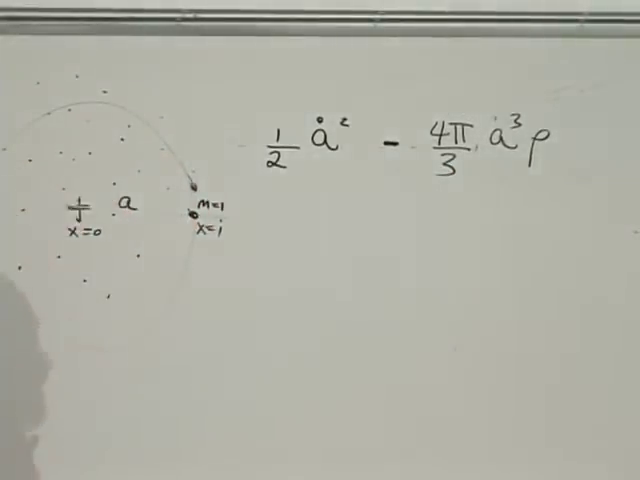
\includegraphics[width=0.78\textwidth]{lecture_03_figure_02.png}
\caption{Esfera homogénea centrada en \(x=0\), una galaxia comóvil en \(x=1\) y el balance de energía newtoniano para \(a(t)\).}
\end{figure}

Solo la materia que está dentro de la esfera de radio \(a(t)\) contribuye a la atracción gravitatoria sobre la partícula en \(x=1\). Asignemos a esa partícula una masa unidad. Su energía cinética es
\begin{equation}
\frac{1}{2}\dot a^2.
\end{equation}
La masa encerrada por la esfera es
\begin{equation}
M_{\mathrm{enc}}=\frac{4\pi}{3}a^3\rho,
\end{equation}
por lo que la energía potencial gravitatoria es
\begin{equation}
-\frac{G M_{\mathrm{enc}}}{a}
=
-\frac{4\pi G}{3}a^2\rho.
\end{equation}
\editorialnote{En la marca de tiempo 00:05:30 de la clase, la pizarra muestra con claridad el término cinético y el término potencial, que depende de la densidad. El coeficiente completo que se escribe aquí se obtiene de la derivación oral.}

La conservación de la energía da
\begin{equation}
\frac{1}{2}\dot a^2-\frac{4\pi G}{3}a^2\rho=\text{const}.
\end{equation}
A continuación, la constante se escribe como \(-k\), con la advertencia habitual de que la normalización estándar solo fija realmente esa notación después de multiplicar la ecuación por \(2\). En la forma estándar,
\begin{equation}
\dot a^2=\frac{8\pi G}{3}a^2\rho-k,
\end{equation}
y al dividir por \(a^2\) se obtiene
\begin{equation}
\left(\frac{\dot a}{a}\right)^2=\frac{8\pi G}{3}\rho-\frac{k}{a^2}.
\end{equation}
Esta es la ecuación de Friedmann en la forma que se utiliza a lo largo de la exposición.

\begin{figure}[ht]
\centering
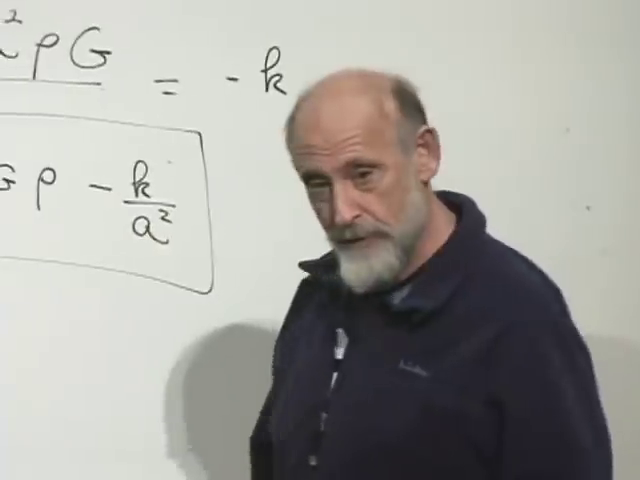
\includegraphics[width=0.56\textwidth]{lecture_03_figure_03.png}
\caption{Contribución de curvatura \(-k/a^2\) aislada en la ecuación de Friedmann.}
\end{figure}

Empíricamente, el término de curvatura es muy próximo a cero; tanto, que a este nivel es muy buena aproximación despreciarlo sin más. Sí corresponde a la curvatura del espacio, pero, desde el punto de vista observacional, aquí es demasiado pequeño incluso para determinar su signo.

La misma ecuación también se obtiene de la relatividad general. Esquemáticamente, la ecuación de Einstein para la componente temporal es
\begin{equation}
R_{00}-\frac{1}{2}g_{00}R \propto T_{00}.
\end{equation}
\editorialnote{Aquí solo se da la estructura tensorial, no el coeficiente numérico global exacto.}
Con una métrica homogénea en expansión, el lado geométrico produce la combinación de \(\dot a/a\) y \(k/a^2\), mientras que el lado de la materia produce la densidad de energía. En esta etapa, el argumento newtoniano y la ecuación de Einstein dicen lo mismo.

Eso también cambia el significado de \(\rho\). De aquí en adelante, es mejor llamar a \(\rho\) la densidad de energía. Para la materia que se mueve lentamente en el sistema comóvil, esta es simplemente la densidad de energía en reposo.

\section{Dominio de la materia}

Supongamos ahora que la densidad de energía se debe a materia en reposo en el sistema comóvil. Consideremos un cubo de una unidad de longitud coordenada por lado. Sus longitudes físicas son \(a(t)\), por lo que su volumen físico es \(a^3(t)\). Si la energía en forma de masa contenida en ese cubo comóvil es \(M\), y la materia se mueve con el flujo en vez de atravesar la frontera, entonces
\begin{equation}
\rho_m=\frac{M}{a^3}.
\end{equation}

Este es el caso dominado por la materia. En esta idealización, las partículas están en reposo dentro de la caja, así que se considera que la temperatura y la presión son cero. Para que haya presión, las partículas tendrían que atravesar la frontera de la caja.

Con \(k\approx 0\), la ecuación queda
\begin{equation}
\left(\frac{\dot a}{a}\right)^2=\frac{8\pi G}{3}\frac{M}{a^3}.
\end{equation}
Probemos una ley potencial,
\begin{equation}
a(t)=Ct^p.
\end{equation}
Entonces
\begin{equation}
\frac{\dot a}{a}=\frac{p}{t},
\end{equation}
De modo que el miembro izquierdo escala como \(t^{-2}\), mientras que el derecho escala como \(t^{-3p}\). Al igualar las potencias se obtiene
\begin{equation}
3p=2,
\qquad
p=\frac{2}{3}.
\end{equation}
Por tanto,
\begin{equation}
a(t)\propto t^{2/3}.
\end{equation}
Al conservar el coeficiente se obtiene
\begin{equation}
C^3=6\pi G M.
\end{equation}

Lo importante de la solución es la ley potencial. Un universo dominado por la materia se expande como la potencia dos tercios del tiempo, no de forma lineal. Esta ley describe una larga etapa intermedia, desde aproximadamente \(10^5\) años después del Big Bang hasta unos pocos miles de millones de años más tarde. El universo actual no está literalmente dominado por la materia, porque ahora domina la energía oscura, pero la materia ordinaria y un largo período de la historia cosmológica se describen de este modo.

\section{Dominio de la radiación}

Antes de esa etapa, la radiación dominaba la densidad de energía. La razón es sencilla. El universo contiene una cantidad enorme de fotones —aproximadamente \(10^9\) por cada protón— y, cuando el universo se comprime, esos fotones adquieren más energía.

Un fotón no tiene masa en reposo, pero sí energía. Su energía es
\begin{equation}
E_\gamma=h\nu=\frac{hc}{\lambda}.
\end{equation}
La hipótesis crucial es que, a medida que el universo se expande, las longitudes de onda de los fotones se estiran con él:
\begin{equation}
\lambda\propto a.
\end{equation}
Una onda dentro de una caja da la imagen adecuada. Si la caja crece, la longitud de onda del modo crece junto con ella. Aquí se aplica la misma idea al universo en expansión.

Como \(\lambda\propto a\), la energía de cada fotón escala como
\begin{equation}
E_\gamma\propto a^{-1}.
\end{equation}
Volvamos a tomar una caja comóvil de una unidad de lado. Los fotones entran y salen, pero, en promedio, el número que hay dentro permanece constante. Así, la energía total de los fotones en la caja también escala como \(a^{-1}\). Al dividirla por el volumen físico \(a^3\), la densidad de energía de la radiación escala como
\begin{equation}
\rho_r\propto a^{-4}.
\end{equation}

Ese factor adicional de \(a^{-1}\) marca toda la diferencia. La materia se diluye porque el universo se expande. La radiación se diluye por esa misma razón y, además, porque cada fotón sufre un corrimiento al rojo.

Por tanto, la ecuación de Friedmann para un universo dominado por la radiación es
\begin{equation}
\left(\frac{\dot a}{a}\right)^2=\frac{8\pi G}{3}\frac{M_r}{a^4}.
\end{equation}
\editorialnote{En la exposición oral se reutiliza el símbolo \(M\) para esta nueva constante. Aquí se añade el subíndice \(r\) solo para evitar confundirla con el caso de la materia.}

Probemos la misma forma \(a(t)=Ct^p\). El miembro izquierdo vuelve a escalar como \(t^{-2}\), mientras que el derecho escala como \(t^{-4p}\). Al igualar las potencias se obtiene
\begin{equation}
4p=2,
\qquad
p=\frac{1}{2}.
\end{equation}
Así que
\begin{equation}
a(t)\propto t^{1/2}.
\end{equation}
Al conservar el coeficiente se obtiene
\begin{equation}
C^4=\frac{32\pi G}{3}M_r.
\end{equation}

\begin{classroomqa}
\lecturetimestamp{00:35:41}
\audiencequestion{¿Por qué aparece un \(G\) ahí?}
\lecturerresponse{Porque lo que gravita es la densidad de energía, no solo la masa en reposo. En el caso de la materia que se mueve lentamente, es fácil pasar por alto la diferencia, pero los fotones nos obligan a tenerla en cuenta: no tienen masa en reposo y, aun así, gravitan.}
\end{classroomqa}

Una caja llena de radiación permite ver la idea con claridad. Empujemos una caja llena de fotones. Cuando la caja acelera, la pared que avanza hacia los fotones recibe impactos más fuertes que la pared que se aleja de ellos, de modo que hay que empujar con más fuerza para vencer la presión de radiación. Por tanto, la caja tiene más inercia y, según el principio de equivalencia, esa inercia adicional también implica más masa gravitatoria. Este es el argumento de la caja de fotones que se emplea aquí para afirmar que la energía gravita.

\begin{classroomqa}
\lecturetimestamp{00:38:11}
\audiencequestion{¿Se puede resolver alguna de estas ecuaciones para un \(a\) que disminuya con el tiempo?}
\lecturerresponse{Sí. Si se reincorpora el término de curvatura \(k/a^2\), hay soluciones en las que el universo se expande y luego se contrae. No parece que eso sea lo que ocurre en nuestro universo, pero la ecuación lo permite.}
\end{classroomqa}

\begin{classroomqa}
\lecturetimestamp{00:38:44}
\audiencequestion{¿Qué pasó con la conservación de la energía?}
\lecturerresponse{Si se reincorpora el término \(k\) y se vuelve a multiplicar la ecuación por \(a^2\), la ecuación cosmológica es precisamente la ley de conservación. La materia o la radiación de un lado son solo una parte del balance. La expansión aporta las partes cinética y gravitatoria, y el balance total se conserva.}
\end{classroomqa}

\section{Materia y radiación juntas}

La cosmología real contiene tanto materia como radiación. Sus densidades escalan de manera distinta:
\begin{equation}
\rho_m\propto a^{-3},
\qquad
\rho_r\propto a^{-4}.
\end{equation}
Así que, para valores pequeños de \(a\), domina la radiación. Para valores grandes de \(a\), domina la materia. Por tanto, al retroceder en el tiempo, se concluye que el universo primitivo estaba dominado por la radiación.

\begin{figure}[ht]
\centering
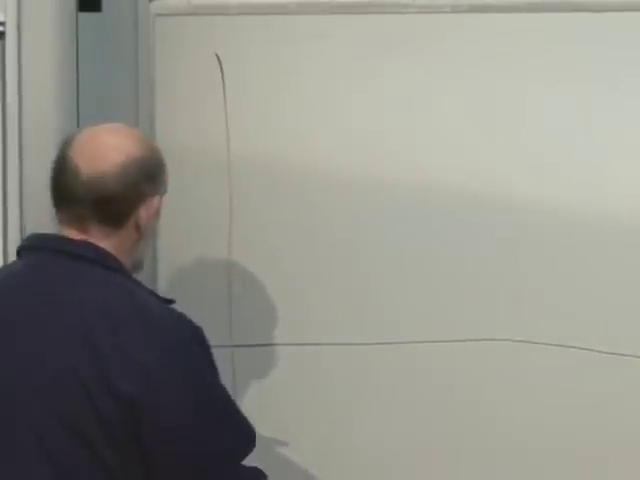
\includegraphics[width=0.68\textwidth]{lecture_03_figure_05.png}
\caption{Ejes para comparar las densidades de energía de la materia y la radiación en función del factor de escala.}
\end{figure}

\editorialnote{En la marca de tiempo 00:44:45 de la clase, la pizarra muestra únicamente los ejes al comienzo de la gráfica comparativa. Las curvas de la materia y la radiación que se analizan inmediatamente después se describen en el texto, pero no se vuelven a dibujar aquí.}

La curva de la materia decrece como \(a^{-3}\). La curva de la radiación decrece como \(a^{-4}\). Ambas divergen cuando \(a\to 0\), pero allí la curva de la radiación crece más deprisa, así que las dos curvas se cruzan en un factor de escala de igualdad. Una estimación aproximada sitúa esta transición después de alrededor de \(10^4\) años, quizá algo más tarde.

La misma idea puede expresarse en la gráfica de \(a(t)\) en función de \(t\). Al principio, la expansión se comporta como \(t^{1/2}\). Más adelante, se comporta como \(t^{2/3}\). El cambio no es un salto, sino una transición continua a lo largo de un intervalo de tiempo relativamente estrecho.

\begin{classroomqa}
\lecturetimestamp{00:44:04}
\audiencequestion{¿La potencia \(p\) pasa de forma continua de \(1/2\) a \(2/3\) a medida que envejece el universo?}
\lecturerresponse{Sí. No hay un salto. El cambio es continuo, aunque ocurre en un intervalo de tiempo bastante estrecho.}
\end{classroomqa}

\section{Temperatura, recombinación y última dispersión}

La siguiente magnitud es la temperatura. Si la energía de un fotón típico escala como \(a^{-1}\), lo mismo ocurre con la temperatura del baño de radiación:
\begin{equation}
T\propto a^{-1}.
\end{equation}
Si \(a\) se duplica, la temperatura se reduce a la mitad.

Tomemos la temperatura actual de los fotones como aproximadamente \(3\,\mathrm K\) y la temperatura de ionización como aproximadamente \(3000\,\mathrm K\), más o menos la temperatura de la superficie del Sol. Entonces
\begin{equation}
\frac{a_{\mathrm{today}}}{a_{\mathrm{ion}}}\sim 10^3.
\end{equation}
Usando la ley de dominio de la materia para tiempos tardíos, \(a\propto t^{2/3}\),
\begin{equation}
\left(\frac{t_{\mathrm{today}}}{t_{\mathrm{ion}}}\right)^{2/3}\sim 10^3,
\end{equation}
por lo que
\begin{equation}
\frac{t_{\mathrm{today}}}{t_{\mathrm{ion}}}\sim 1000^{3/2}\sim 3\times 10^4.
\end{equation}
Si para esta estimación tomamos que la edad del universo es \(10^{10}\) años, obtenemos
\begin{equation}
t_{\mathrm{ion}}\sim 3\times 10^5\ \mathrm{years}.
\end{equation}

Esta es la época en que el hidrógeno y el helio dejan de estar completamente ionizados. Antes de entonces, el universo es un plasma caliente. ¿Por qué es opaco un plasma? Porque las cargas libres responden con fuerza a las ondas electromagnéticas. El campo eléctrico hace oscilar las cargas, el medio se comporta como un conductor y los conductores son opacos. Esa es la analogía pertinente con la superficie del Sol.

Cuando el universo se enfría lo suficiente para que los electrones se recombinen con los núcleos, se forman átomos neutros ordinarios y el universo se vuelve mucho más transparente. La transición no es infinitamente abrupta. Ocurre en una región o un intervalo de tiempo difusos, pero es lo bastante definida para la cosmología como para llamarla superficie de última dispersión.

Mirar hacia el exterior significa mirar hacia atrás en el tiempo. Las galaxias cercanas muestran el pasado reciente. Las galaxias más lejanas muestran épocas anteriores. A suficiente distancia, todas las líneas de visión llegan a la época en que el universo aún estaba ionizado y era opaco. La radiación electromagnética no puede mostrarnos nada anterior a esa época.

En principio, otros mensajeros podrían permitir explorar épocas anteriores. Los neutrinos son eléctricamente neutros y se desacoplarían antes. Los gravitones, si algún día se pudieran observar, procederían de épocas aún más tempranas. Pero la misma debilidad de la interacción que les permitiría atravesar el plasma primitivo también los hace extremadamente difíciles de detectar.

Si en algún momento el universo estuvo tan caliente como la superficie del Sol en todas direcciones, ¿por qué el cielo no brilla con una intensidad cegadora? Porque la superficie de última dispersión se aleja, y los fotones que nos llegan desde ella han sufrido un corrimiento al rojo por un factor aproximadamente igual a \(10^3\), que es la razón entre \(3000\,\mathrm K\) y \(3\,\mathrm K\). Lo que nos llega es radiación de microondas, no luz solar visible.

\begin{classroomqa}
\lecturetimestamp{01:03:51}
\audiencequestion{¿Entonces nuestros telescopios no pueden observar épocas anteriores a unos \(300{,}000\) años?}
\lecturerresponse{Los telescopios electromagnéticos no pueden. Antes de esa época, el universo estaba ionizado y era opaco. En principio, otros mensajeros podrían permitir explorar épocas anteriores.}
\end{classroomqa}

\begin{classroomqa}
\lecturetimestamp{01:08:43}
\audiencequestion{Cuando hablas de la temperatura de un fotón, te refieres a la temperatura de un cuerpo negro cuya radiación tiene ese pico. Pero no depende linealmente de la longitud de onda, ¿verdad?}
\lecturerresponse{Exacto. La temperatura corresponde, en esencia, a la energía de un fotón típico, de modo que, para un fotón, es inversamente proporcional a la longitud de onda. La ley \(T^4\) se refiere a la densidad de energía, no a la energía de un solo fotón. Combina la energía por fotón con el número de fotones por unidad de volumen, y la densidad numérica escala como \(T^3\).}
\end{classroomqa}

Por tanto,
\begin{equation}
n_\gamma\propto T^3,
\qquad
\rho_\gamma\propto T^4.
\end{equation}

\section{Materia oscura a partir de las curvas de rotación}

La materia oscura aparece al estudiar las curvas de rotación galácticas. No se infirió a partir de la ecuación de Friedmann a gran escala, sino de observaciones astronómicas a escala galáctica.

Empecemos con el problema newtoniano más sencillo: un cuerpo ligero de masa \(m\) que orbita una masa central \(M\) a un radio \(r\). La fuerza gravitatoria es
\begin{equation}
\frac{GMm}{r^2},
\end{equation}
y la aceleración centrípeta es \(v^2/r\). La ley de Newton da
\begin{equation}
m\frac{v^2}{r}=\frac{GMm}{r^2}.
\end{equation}
Se simplifica \(m\), se multiplica por \(r\) y se obtiene
\begin{equation}
v(r)=\sqrt{\frac{GM}{r}}.
\end{equation}
Así que, si la masa gravitatoria está concentrada cerca del centro, la velocidad orbital decrece como \(r^{-1/2}\).

Eso es lo que cabría esperar si la masa siguiera la luz. La mayor parte de la materia visible de una galaxia se encuentra cerca del núcleo, así que, en ese caso, las estrellas exteriores se comportarían de forma muy parecida a los planetas de las regiones externas del sistema solar. Los astrónomos infieren las velocidades orbitales midiendo las diferencias de corrimiento Doppler a través de una galaxia cercana: comparan el lado que se mueve hacia nosotros con el que se aleja, una vez descontado el movimiento recesivo global de la galaxia. Las velocidades orbitales medidas se mantienen aproximadamente constantes hasta radios grandes.

Así que sustituyamos la masa central \(M\) por la masa encerrada \(M(r)\):
\begin{equation}
\frac{v^2}{r}=\frac{G M(r)}{r^2}.
\end{equation}
Si \(v(r)\) es aproximadamente constante, entonces
\begin{equation}
M(r)\propto r.
\end{equation}
En otras palabras, la masa gravitatoria sigue aumentando con el radio incluso en regiones donde la luz visible no lo hace.

Supongamos ahora, como se hace por simplicidad en la exposición, que la distribución de masa es aproximadamente esférica. Entonces
\begin{equation}
M(R)=\int_0^R 4\pi r^2\rho(r)\,dr.
\end{equation}
Si \(M(R)\propto R\), al derivar con respecto a \(R\) se obtiene
\begin{equation}
4\pi R^2\rho(R)\propto 1,
\end{equation}
y, por tanto,
\begin{equation}
\rho(r)\propto \frac{1}{r^2}.
\end{equation}

\begin{classroomqa}
\lecturetimestamp{01:28:18}
\audiencequestion{Parece que la densidad debería variar como \(1/r^2\). ¿Hay alguna razón para ello?}
\lecturerresponse{A partir de la curva de rotación plana observada se infiere \(M(R)\propto R\), y al derivar se obtiene \(\rho(r)\propto 1/r^2\). Más allá de eso, aquí no se propone ninguna explicación sencilla basada en primeros principios; las simulaciones detalladas hacen gran parte del trabajo.}
\end{classroomqa}

La conclusión firme es que una galaxia contiene mucha más masa gravitatoria de la que sugeriría la materia luminosa por sí sola: varias veces más y, según la estimación utilizada aquí, aproximadamente un orden de magnitud más. La galaxia visible está dentro de un halo oscuro mucho mayor.

¿Qué impide que el gas ordinario permanezca en un estado tan difuso? La disipación. Una nube de gas se contrae porque las colisiones, los procesos similares a la fricción y la radiación le permiten perder energía. Al parecer, la materia oscura no emite una cantidad apreciable de radiación y es casi no colisional. La gravedad puede atraerla hacia dentro y convertir energía potencial en energía cinética, pero, sin una disipación eficiente, no colapsa para formar las estructuras luminosas compactas que forma la materia ordinaria. Lo que mantiene extendido el halo es la energía cinética.

A continuación se analizan con cautela varias alternativas. Se dice que los neutrinos son demasiado rápidos para comportarse así a escala galáctica. Un halo compuesto de hidrógeno ordinario alteraría gravemente la nucleosíntesis del universo primitivo. También se menciona que los agujeros negros formados por materia ordinaria plantean problemas, porque implicarían demasiada materia ordinaria en el universo primitivo y suscitarían problemas de lente gravitatoria; la exposición no afirma nada más en ese momento.

El halo no se describe como una cáscara delgada ni como un toro. Es una distribución aproximadamente esférica y no uniforme, más densa hacia el centro y cada vez menos densa hacia el exterior.

\begin{classroomqa}
\lecturetimestamp{01:53:12}
\audiencequestion{¿Te refieres al Cúmulo Bala?}
\lecturerresponse{Sí. El gas de rayos X muestra la materia ordinaria, mientras que las lentes gravitatorias muestran la masa gravitatoria total. En la colisión, esas dos distribuciones se separan. Es una prueba sólida de que la materia oscura es real, y no una mera modificación de la gravedad vinculada exclusivamente a la materia visible.}
\end{classroomqa}

Ese es el último punto observacional. Se sabe muy poco en detalle sobre qué es la materia oscura, pero nada de lo expuesto requiere un principio radicalmente nuevo. La posibilidad más conservadora es, sencillamente, que la naturaleza contenga partículas adicionales que interactúan débilmente y que aún no se han identificado.

\chapter{Horizontes, ecuación de estado y energía del vacío}

\section{Marco preferente, recesión superlumínica y horizonte}

La radiación cósmica de fondo de microondas sí determina un marco especial. En el marco en que esa radiación se observa isotrópica, las galaxias cercanas también están, en promedio, en reposo. Si nos movemos a través del fondo, los fotones que llegan de frente experimentan un desplazamiento Doppler hacia energías mayores, y los que llegan desde atrás, hacia energías menores. El marco preferente es aquel en que el fondo de microondas se observa isotrópico y, además, es también, en promedio, el marco en que las galaxias locales están en reposo.

\begin{classroomqa}
\lecturetimestamp{00:00:25}
\audiencequestion{¿La longitud de onda aparente de la radiación cósmica depende del movimiento del observador? ¿Implica eso que existe un marco preferente?}
\lecturerresponse{Sí. El movimiento a través del fondo de microondas produce una anisotropía Doppler, así que existe un marco cosmológico preferente: aquel en que el fondo de microondas se observa isotrópico. Además, es también, en promedio, el marco en que las galaxias locales están en reposo.}
\end{classroomqa}

Una segunda cuestión se refiere a las velocidades de recesión. La ley de Hubble dice que galaxias suficientemente distantes se separan de acuerdo con
\begin{equation}
v = H d .
\end{equation}
Para valores suficientemente grandes de \(d\), esta velocidad de recesión supera la velocidad de la luz. Esto no contradice la relatividad, porque la prohibición es local: un objeto no puede pasar junto a otro, justo delante de nosotros, a una velocidad superior a la de la luz. La afirmación sobre galaxias distantes se refiere a la geometría entre lugares muy separados.

\begin{classroomqa}
\lecturetimestamp{00:04:48}
\audiencequestion{¿Pueden dos galaxias tener una velocidad relativa mayor que \(c\)?}
\lecturerresponse{Sí, si están lo bastante alejadas. La recesión de Hubble puede superar la velocidad de la luz sin violar la relatividad local; el lugar donde la velocidad de recesión alcanza \(c\) es un horizonte.}
\end{classroomqa}

Cuando la recesión alcanza la velocidad de la luz, las señales enviadas hacia nosotros dejan de acercarse en términos netos. El rayo sigue moviéndose localmente a la velocidad límite, pero la distancia que debe recorrer crece demasiado deprisa.

\begin{classroomqa}
\lecturetimestamp{00:07:03}
\audiencequestion{¿No seguiría viajando hacia nosotros un rayo de luz enviado en sentido contrario?}
\lecturerresponse{Localmente sí, pero el espacio se expande más deprisa de lo que el rayo puede avanzar. El rayo se mueve a la velocidad límite respecto a los puntos cercanos, mientras que la distancia total hasta nosotros sigue aumentando.}
\end{classroomqa}

\section{La métrica en expansión y la analogía de la línea}

Una imagen útil es la de una dimensión. Imaginemos una línea formada por átomos. Si estiramos una línea de material corriente, al final se rompe. Modifiquemos ahora la imagen: cada vez que los átomos vecinos se separan demasiado, insertamos otro entre ellos. La línea sigue creciendo, pero sus propiedades locales no se diluyen.

\begin{figure}
\centering
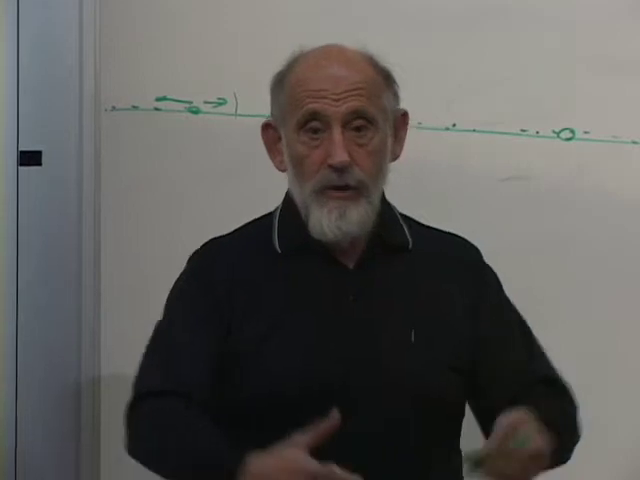
\includegraphics[width=0.60\textwidth]{lecture_04_figure_02.png}
\caption{Línea unidimensional utilizada para representar una métrica en expansión.}
\end{figure}

En esta imagen sigue habiendo una velocidad límite local para las señales, igual que el sonido tiene una velocidad límite en una línea corriente. La regla es local: una perturbación no puede superar esa velocidad respecto a los puntos cercanos. Sin embargo, si la línea es lo bastante larga y se insertan puntos nuevos con suficiente rapidez, las partes suficientemente distantes se alejan tan deprisa que una señal nunca puede regresar.

Por tanto, la suma de velocidades de la relatividad especial es solo una parte de la historia. Se aplica localmente, cuando los observadores pasan uno junto al otro en el mismo punto. No es la herramienta adecuada para describir galaxias muy separadas en una geometría en expansión.

\begin{classroomqa}
\lecturetimestamp{00:09:42}
\audiencequestion{¿Sigue siendo válida en esta situación la ley relativista habitual de suma de velocidades?}
\lecturerresponse{Localmente, en un punto, sí. Si los observadores pasan uno junto al otro, uno tras otro, se aplica la regla habitual de la relatividad especial. Pero no es la manera adecuada de describir una recesión superlumínica entre objetos muy separados; en ese caso hay que volver a la geometría del espacio en expansión.\(c\)
}
\end{classroomqa}

La misma imagen ofrece una explicación sencilla del corrimiento al rojo. Dibujemos una onda sobre la línea. Al expandirse la línea, también aumenta la longitud de onda. En una geometría en expansión, no se trata solo de una imagen sugerente: las ecuaciones de onda en un espacio-tiempo en expansión producen realmente longitudes de onda estiradas.

\begin{classroomqa}
\lecturetimestamp{00:14:42}
\audiencequestion{¿La afirmación de que una onda se estira junto con el universo es teórica, empírica o ambas cosas?}
\lecturerresponse{Es una consecuencia teórica de la propagación de ondas en un espacio-tiempo en expansión y, además, cuenta con el respaldo de las observaciones astronómicas.}
\end{classroomqa}

Esta imagen no representa una banda elástica. Al estirarla, una banda elástica se hace más delgada, y alguien que viviera en ese medio vería cambiar sus propiedades locales. Aquí las propiedades locales permanecen iguales mientras crece la escala global de distancias.

\section{La última dispersión y el universo observable}

El horizonte es el lugar donde la recesión alcanza la velocidad de la luz. La superficie de última dispersión se encuentra ligeramente dentro de él. Una señal emitida desde el horizonte sufriría un corrimiento al rojo ilimitado; la radiación de última dispersión tiene un corrimiento al rojo enorme, pero finito.

\begin{classroomqa}
\lecturetimestamp{00:17:53}
\audiencequestion{¿Qué relación hay entre la recesión superlumínica, la superficie de última dispersión y el universo observable?}
\lecturerresponse{El horizonte es el lugar donde la recesión alcanza la velocidad de la luz. La superficie de última dispersión se encuentra ligeramente dentro de él porque su corrimiento al rojo es enorme, pero finito. A efectos prácticos, marca el borde del universo observable.}
\end{classroomqa}

El corrimiento al rojo de la radiación de última dispersión es, aproximadamente, un factor \(10^3\). Es un valor tan grande que, para muchos propósitos, la superficie de última dispersión está muy cerca del horizonte. El universo observable es la parte del universo desde la que la luz puede llegar hasta nosotros.

En tiempos tardíos, la expansión se aproxima al régimen dominado por el vacío. Entonces la magnitud de Hubble tiende a una constante, el horizonte se aproxima a un tamaño fijo y tanto las galaxias como la radiación de microondas van desapareciendo progresivamente de nuestra vista.

\begin{classroomqa}
\lecturetimestamp{00:22:43}
\audiencequestion{Puesto que \(H\) cambia con el tiempo, ¿cambia también la distancia al horizonte? ¿Acabará desapareciendo el fondo de microondas?}
\lecturerresponse{En tiempos tardíos, \(H\) tiende a una constante, así que el horizonte se aproxima a una distancia fija. El fondo de microondas sigue estirándose, enfriándose y desvaneciéndose. Las galaxias distantes también atraviesan el horizonte y desaparecen de nuestra vista.}
\end{classroomqa}

Solo permanecen visibles las estructuras que ya están ligadas gravitatoriamente. El sistema solar no se desintegra, ni tampoco la galaxia, pero el universo a gran escala se convierte en una isla aislada.

\section{La ecuación básica de expansión y los tres componentes}

La ecuación básica de expansión es ahora
\begin{equation}
\left(\frac{\dot a}{a}\right)^2 = \frac{8\pi G}{3}\rho ,
\qquad c=1 .
\end{equation}
Aquí \(a(t)\) es el factor de escala y \(\rho\) es la densidad de energía total.

\begin{figure}
\centering
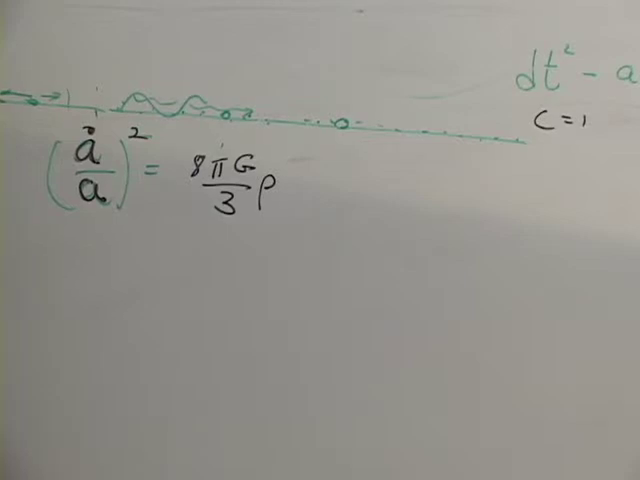
\includegraphics[width=0.74\textwidth]{lecture_04_figure_03.png}
\caption{Ecuación básica de expansión junto con la analogía de la línea unidimensional.}
\end{figure}

Hay tres componentes dinámicamente importantes.

Para la materia,
\begin{equation}
\rho=\frac{\text{const.}}{a^3},
\qquad
a(t)\sim t^{2/3}.
\end{equation}
Este es el caso de objetos masivos que se mueven con la expansión global y que están esencialmente en reposo en el marco comóvil.

Para la radiación,
\begin{equation}
\rho=\frac{\text{const.}}{a^4},
\qquad
a(t)\sim t^{1/2}.
\end{equation}
La potencia adicional de \(a\) se debe al corrimiento al rojo que experimenta cada fotón al expandirse el universo.

También hay
\begin{equation}
\rho_0=\text{constant},
\end{equation}
energía del vacío, también llamada energía oscura o, salvo factores numéricos convencionales, constante cosmológica. Este componente no se diluye en absoluto.

El siguiente paso es relacionar la densidad de energía con la presión.

\section{La presión de radiación y la materia fría}

Empecemos por la radiación. Consideremos una caja unidimensional, solo un segmento de longitud \(L\), que contiene fotones rebotando de un lado a otro. En una dimensión, fuerza y presión son, en la práctica, lo mismo.

Tomemos un fotón cuyo módulo del momento es \(p\). Cuando se refleja en una pared, su momento cambia en
\begin{equation}
\Delta p = 2p.
\end{equation}
El tiempo entre colisiones sucesivas con la misma pared es
\begin{equation}
\Delta t = \frac{2L}{c}.
\end{equation}
Por tanto, la fuerza media sobre la pared es
\begin{equation}
F=\frac{\Delta p}{\Delta t}=\frac{pc}{L}.
\end{equation}
Para un fotón,
\begin{equation}
E=pc,
\end{equation}
así que
\begin{equation}
F=\frac{E}{L}.
\end{equation}
La energía dividida por la longitud es la densidad de energía unidimensional. En este caso unidimensional,
\begin{equation}
P=\rho .
\end{equation}

Con muchos fotones, la misma relación se mantiene al promediar. La fuerza total es simplemente la energía total por unidad de longitud.

Pasemos ahora a tres dimensiones. Si todos los fotones se movieran solo a lo largo de un eje, ejercerían presión sobre un par de caras y ninguna sobre las demás. Este supuesto es deliberadamente incorrecto, pero muestra enseguida qué hay que corregir. En un baño isotrópico, el momento se distribuye en todas las direcciones. En promedio, un tercio de la densidad de energía contribuye a cada componente de la presión. El resultado es
\begin{equation}
P=\frac{\rho}{3}.
\end{equation}

Para la materia fría, el resultado es distinto. Tomemos una caja comóvil, una pequeña región que se mueve con el flujo del universo. Las partículas de su interior tienen energía, pero, si están en reposo respecto a la caja, no chocan contra sus paredes. Por tanto, la presión es
\begin{equation}
P=0.
\end{equation}

\begin{figure}
\centering
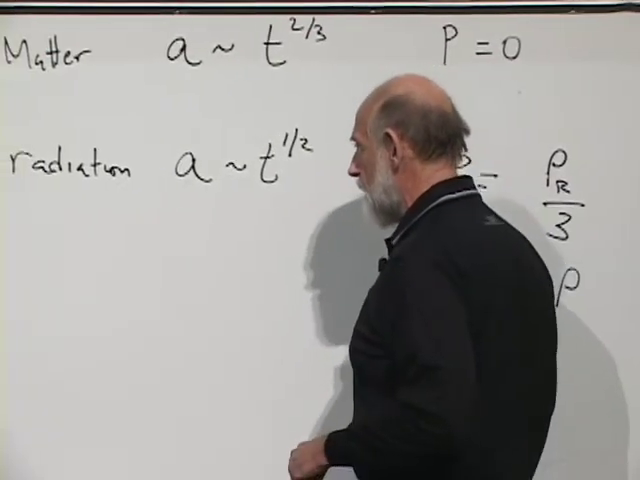
\includegraphics[width=0.74\textwidth]{lecture_04_figure_04.png}
\caption{Materia y radiación: \(a\sim t^{2/3}\), \(P=0\) y \(a\sim t^{1/2}\), \(P=\rho/3\).}
\end{figure}

El resumen de la pizarra es
\begin{align}
\text{matter:}\qquad & a(t)\sim t^{2/3}, \qquad P=0,\\
\text{radiation:}\qquad & a(t)\sim t^{1/2}, \qquad P=\frac{\rho}{3}.
\end{align}

\begin{classroomqa}
\lecturetimestamp{00:54:27}
\audiencequestion{En el universo en expansión, ¿no se están separando realmente las partículas?}
\lecturerresponse{Sí, pero el argumento sobre la presión se aplica a una caja comóvil infinitesimal. A esa escala local, el razonamiento termodinámico sigue siendo válido.}
\end{classroomqa}

\section{La ecuación de estado}

Se supone que la presión es proporcional a la densidad de energía:
\begin{equation}
P=w\rho .
\end{equation}
En la pizarra, el mismo parámetro se escribe como \(\omega\). Para los dos casos básicos,
\begin{equation}
w=0 \quad \text{for cold matter},
\qquad
w=\frac{1}{3} \quad \text{for radiation}.
\end{equation}

También son posibles los casos intermedios. Los valores comprendidos entre \(0\) y \(1/3\) describen materia que no es ni completamente fría ni plenamente relativista. Aquí se menciona como ejemplo la materia oscura caliente.

\begin{figure}
\centering
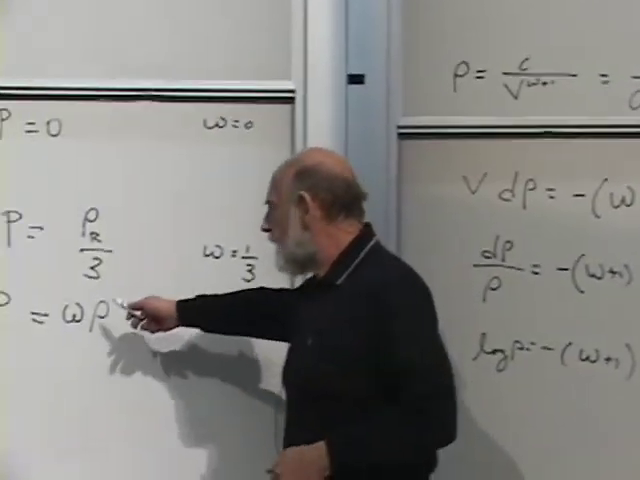
\includegraphics[width=0.74\textwidth]{lecture_04_figure_05.png}
\caption{Ecuación de estado \(P=\omega\rho\) junto con el argumento sobre la escala de la densidad.}
\end{figure}

La siguiente cuestión es si \(w\) determina la dependencia de \(\rho\) respecto de \(a\). La respuesta se obtiene de una identidad termodinámica.

Tomemos una caja de volumen \(V\). Si su contenido ejerce una presión \(P\), cuando la caja se expande en \(dV\), el trabajo realizado sobre sus paredes es
\begin{equation}
dE=-P\,dV.
\end{equation}
Escribamos ahora la energía como
\begin{equation}
E=\rho V.
\end{equation}
Su diferencial es
\begin{equation}
dE=\rho\,dV+V\,d\rho .
\end{equation}
Al igualar las dos expresiones se obtiene
\begin{equation}
\rho\,dV+V\,d\rho=-P\,dV,
\end{equation}
o bien
\begin{equation}
V\,d\rho=-(\rho+P)\,dV.
\end{equation}
Usando \(P=w\rho\),
\begin{equation}
V\,d\rho=-(1+w)\rho\,dV.
\end{equation}
Dividamos por \(\rho V\):
\begin{equation}
\frac{d\rho}{\rho}=-(1+w)\frac{dV}{V}.
\end{equation}
Al integrar,
\begin{equation}
\rho \propto V^{-(1+w)}.
\end{equation}
Para una caja cosmológica comóvil,
\begin{equation}
V\propto a^3,
\end{equation}
y, por tanto,
\begin{equation}
\rho \propto a^{-3(1+w)}.
\end{equation}

Se recuperan enseguida los casos anteriores:
\begin{align}
w=0 &\Longrightarrow \rho \propto a^{-3},\\
w=\frac{1}{3} &\Longrightarrow \rho \propto a^{-4}.
\end{align}

Por eso importa \(w\). Una vez conocida \(\rho(a)\), se puede sustituir en la ecuación de Friedmann. Después se prueba una ley de potencias \(a\sim t^\alpha\) y se determina cómo se expande el universo para esa ecuación de estado.

\section{Energía del vacío y presión negativa}

Un caso especial se comporta de manera distinta:
\begin{equation}
w=-1.
\end{equation}
Entonces
\begin{equation}
1+w=0,
\end{equation}
por lo que el exponente se anula y
\begin{equation}
\rho=\rho_0=\text{constant}.
\end{equation}
La presión correspondiente es
\begin{equation}
P=-\rho .
\end{equation}

La presión negativa no tiene nada de misterioso por sí misma. La presión positiva empuja hacia fuera las paredes de una caja. La negativa tira de ellas hacia dentro. Es tensión. Una banda elástica estirada es un ejemplo cotidiano: almacena energía positiva, pero tira de sus extremos para juntarlos.

Sustituyamos la densidad constante \(\rho_0\) en la ecuación de Friedmann:
\begin{equation}
\left(\frac{\dot a}{a}\right)^2=\frac{8\pi G}{3}\rho_0.
\end{equation}
El miembro derecho es simplemente un número, así que
\begin{equation}
\frac{\dot a}{a}=\sqrt{\frac{8\pi G}{3}\rho_0}.
\end{equation}
Este es el caso especial en que la magnitud de Hubble sí es constante. La ecuación puede escribirse como
\begin{equation}
\dot a=\sqrt{\frac{8\pi G}{3}\rho_0}\,a,
\end{equation}
y la solución es
\begin{equation}
a(t)\propto \exp\!\left(\sqrt{\frac{8\pi G}{3}\rho_0}\,t\right).
\end{equation}

Esta es una expansión exponencial. La escala de tiempo pertinente es el tiempo de crecimiento por un factor \(e\), no el tiempo de duplicación; la estimación aproximada utilizada aquí lo sitúa en el orden de la edad del universo. La energía del vacío y la constante cosmológica son el mismo ingrediente físico, salvo por convenciones numéricas históricas.

\begin{classroomqa}
\lecturetimestamp{01:27:16}
\audiencequestion{Si la energía del vacío impulsa una expansión exponencial, ¿no acabará todo desgarrado?}
\lecturerresponse{No necesariamente. Los sistemas ligados pueden resistirla. Una galaxia, un sistema solar o un átomo no tienen por qué desgarrarse, mientras que las estructuras suficientemente grandes y poco densas sí participan en la expansión y acaban separándose.}
\end{classroomqa}

\begin{classroomqa}
\lecturetimestamp{01:31:43}
\audiencequestion{¿Tiene algún significado el signo negativo al extraer la raíz cuadrada de la ecuación de Friedmann?}
\lecturerresponse{Sí. La raíz cuadrada da dos ramas. Una corresponde a la solución en expansión y la otra a la solución en contracción, que es su reversión temporal. Las propias ecuaciones admiten ambas.}
\end{classroomqa}

\section{Tres eras y la historia de expansión observada}

Los tres componentes están presentes y su densidad evoluciona de manera distinta:
\begin{equation}
\begin{aligned}
\rho_{\text{radiation}}&\propto a^{-4},\\
\rho_{\text{matter}}&\propto a^{-3},\\
\rho_0&=\text{constant}.
\end{aligned}
\end{equation}
De ahí se deducen inmediatamente tres eras.

Para valores muy pequeños de \(a\), domina la radiación. Más adelante domina la materia. Para valores suficientemente grandes de \(a\), domina la energía del vacío. Las leyes de expansión correspondientes son
\begin{equation}
a(t)\sim t^{1/2},
\qquad
a(t)\sim t^{2/3},
\qquad
a(t)\sim e^{Ht}.
\end{equation}

Los tiempos aproximados que se citan aquí son los siguientes: la radiación deja paso a la materia después de unos \(10^4\) años. El universo se vuelve transparente más tarde, después de unos \(10^5\) años. La transición del dominio de la materia a la expansión acelerada ocurre mucho más tarde, después de varios miles de millones de años, aproximadamente a mitad de la historia cósmica según la estimación de orden de magnitud que se utiliza.

¿Cómo se infiere esta historia? No podemos ver el futuro, pero sí el pasado. Mirar a mayor distancia equivale a mirar a épocas anteriores. Al observar galaxias distantes, medir cómo se relaciona su movimiento con la distancia y reconstruir la magnitud de Hubble en función del tiempo retrospectivo, se reconstruye la evolución temporal del factor de escala. La era dominada por la radiación es demasiado temprana para observarla directamente mediante la astronomía galáctica ordinaria, pero la era dominada por la materia y la transición al dominio del vacío sí se aprecian en la curva reconstruida.

\section{La última dispersión en el futuro lejano}

La evolución futura del cielo de microondas no es lo mismo que la desaparición de las galaxias al atravesar el horizonte. La radiación que vemos en épocas posteriores procede de materia más distante, así que el efecto es observar regiones más profundas y frías, en lugar de ver cómo los mismos átomos se alejan sin más.

\begin{classroomqa}
\lecturetimestamp{01:48:07}
\audiencequestion{Si la superficie de última dispersión se desvanece en el horizonte, ¿es eso lo mismo que las galaxias que se alejan más allá del horizonte?}
\lecturerresponse{No. La radiación posterior no procede de los mismos átomos que la que vemos ahora. Procede de átomos que estaban más lejos, así que es como observar regiones cada vez más profundas del universo, mientras la radiación se ve cada vez más fría.}
\end{classroomqa}

\section{Curvatura, la imagen del gran colapso y el horizonte en tiempos tardíos}

Hasta ahora se había omitido el término de curvatura. Al recuperarlo, se obtiene
\begin{equation}
\left(\frac{\dot a}{a}\right)^2
=
\frac{8\pi G}{3}\rho
-
\frac{K}{a^2}.
\end{equation}
Numéricamente, este término parece pequeño, pero conceptualmente es importante. En el lenguaje newtoniano antiguo, distingue los casos de energía total positiva, nula y negativa. En el lenguaje relativista, distingue las geometrías espaciales.

Antes de que se tomara en serio la energía del vacío, se solía imaginar un universo dominado por la materia en que la expansión acabaría invirtiéndose. De ahí surgió la antigua imagen del gran colapso: expansión desde el Big Bang y, después, recontracción. Las matemáticas siguen siendo válidas, pero ya no parece que describan nuestro universo.

\begin{classroomqa}
\lecturetimestamp{01:53:51}
\audiencequestion{¿Está relacionada esta energía del vacío con la energía del vacío cuántico?}
\lecturerresponse{Sí, o al menos eso se cree.}
\end{classroomqa}

La composición aproximada actual es
\begin{equation}
\frac{\rho_0}{\rho_{\text{total}}}\sim 0.7,
\qquad
\frac{\rho_{\text{matter}}}{\rho_{\text{total}}}\sim 0.3.
\end{equation}
De ese componente de materia, la materia luminosa representa aproximadamente \(0.05\) del total y la materia oscura, aproximadamente \(0.25\). Hoy en día, la radiación es despreciable. La materia oscura y la luminosa evolucionan de la misma manera, así que su proporción permanece fija, aunque la abundancia relativa de materia, radiación y vacío cambie de una era a otra.

En el límite dominado por el vacío,
\begin{equation}
H=\sqrt{\frac{8\pi G}{3}\rho_0}.
\end{equation}
La ley de Hubble queda entonces
\begin{equation}
v=Hd.
\end{equation}
El horizonte se define mediante \(v=1\), así que su distancia es
\begin{equation}
d_H=\frac{1}{H}
=
\frac{1}{\sqrt{8\pi G\rho_0/3}}.
\end{equation}
La cifra aproximada que se da aquí es de \(10\) a \(12\) mil millones de años luz.

Lo importante es el comportamiento en tiempos tardíos. Una vez que la expansión es exponencial, la distancia al horizonte se vuelve fija. Las galaxias siguen atravesándolo y desaparecen al sufrir un corrimiento al rojo cada vez mayor. El fondo de microondas también queda desplazado al rojo hasta desaparecer. En el futuro remoto, solo permanecen visibles las estructuras cercanas ligadas gravitatoriamente, y el universo parece una isla aislada.

\section{Geometría a partir de la superficie de última dispersión}

Por último, se puede poner a prueba la geometría a partir de la superficie de última dispersión. Supongamos que se conoce la distancia hasta esa superficie. Supongamos también que se puede identificar allí una concentración de tamaño físico suficientemente conocido. Entonces se pueden comparar ese tamaño y esa distancia con el tamaño angular observado.

En un espacio plano, el ángulo es el euclidiano. En un espacio con curvatura positiva, el objeto parecería mayor; con curvatura negativa, menor. La analogía es la topografía corriente: se toma un objeto de tamaño y distancia conocidos y se compara el ángulo medido con el que predice la geometría euclidiana.

\begin{classroomqa}
\lecturetimestamp{02:08:09}
\audiencequestion{¿Qué ejemplo hay de un objeto ahí fuera cuyo tamaño conozcamos?}
\lecturerresponse{Las concentraciones más grandes del fondo de microondas. Creemos conocer su tamaño a partir del tiempo que tardaron en evolucionar y de la velocidad del sonido.}
\end{classroomqa}

Los objetos pertinentes aquí son las concentraciones más grandes del fondo de microondas. Su tamaño angular observado concuerda con la geometría euclidiana con una diferencia de unos pocos puntos porcentuales. Sobre esa base, el espacio parece plano.

\section{El valor medido de \(w\) y una última pregunta}

Ahora está clara la importancia observacional de \(w\). Si los astrónomos informan de que \(w\) es muy cercano a \(-1\), están diciendo que el componente de energía del vacío es prácticamente constante. Ese es exactamente el punto que se plantea aquí.

Eso no significa que la relatividad general obligue a que \(w\) sea exactamente \(-1\). El argumento que se plantea aquí es empírico. La clase menciona brevemente que, en principio, no se descartan posibilidades más radicales, pero que hay buenos motivos para creer en el caso de una energía del vacío casi constante.

\begin{classroomqa}
\lecturetimestamp{02:11:04}
\audiencequestion{Al calcular la densidad de la materia y de la radiación, ¿supusimos que la energía era constante y luego ajustamos el factor de escala para obtener la fórmula? Y, si eso es así para los dos primeros casos, ¿qué ocurre en el caso de la energía del vacío, en que la densidad permanece constante?}
\lecturerresponse{No. No supuse que fuera constante. Usamos que la variación de energía es \(-P\,dV\). Para una caja comóvil imaginaria que se mueve junto con la expansión, se realiza trabajo sobre las paredes, y eso explica la variación de energía. El caso de la energía del vacío plantea la cuestión de otra manera, y la observación final aquí es que hablar de conservación de la energía en cosmología no dice mucho, porque la energía total del universo es cero.}
\end{classroomqa}

\chapter{Esferas, espacio hiperbólico y significado de \(k\)}

Veamos un poco de matemáticas, unas matemáticas sencillas. Las esferas de cualquier número de dimensiones son geometrías especiales: son homogéneas, y aquí homogéneo significa de curvatura constante. Primero veremos la curvatura positiva, luego la curvatura negativa uniforme y, después, la conexión con las ecuaciones de Einstein.

Un universo esférico significa que \emph{el espacio} es esférico, no el espacio-tiempo. También existe la posibilidad de una curvatura negativa uniforme. Al poner estos casos uno junto al otro se aclara el papel de la relatividad general.

\section{Esferas y geometría uniforme}

Una esfera de dimensión uno no es más que un círculo. La forma más sencilla de describirla es embeberla en un espacio auxiliar de dos dimensiones y escribir
\begin{equation}
x^2+y^2=R^2.
\end{equation}
La esfera unitaria de dimensión uno es
\begin{equation}
x^2+y^2=1.
\end{equation}

Una esfera de dimensión dos se describe del mismo modo, ahora con tres coordenadas auxiliares:
\begin{equation}
x^2+y^2+z^2=R^2,
\end{equation}
En el caso unitario,
\begin{equation}
x^2+y^2+z^2=1.
\end{equation}

Estas coordenadas son solo un recurso auxiliar. La geometría que nos interesa no es la del espacio circundante \(x,y,z\). Es la de la propia superficie. Una criatura que vive en una esfera de dimensión uno vive en un círculo; no tiene acceso a un interior ni a un exterior. La misma idea se aplica a una esfera de dimensión dos. El interior de la esfera y su exterior pertenecen únicamente a la representación auxiliar.

La misma construcción da lugar a una esfera de dimensión tres. Se introduce una coordenada más, por ejemplo \(w\), y se escribe
\begin{equation}
x^2+y^2+z^2+w^2=R^2,
\end{equation}
En el caso unitario,
\begin{equation}
x^2+y^2+z^2+w^2=1.
\end{equation}
Una esfera de dimensión tres es más difícil de visualizar, porque el recurso auxiliar tendría ahora cuatro dimensiones, pero las matemáticas no son mucho más difíciles.

La notación estándar es \(\Omega_n\) para la esfera de dimensión \(n\). Así, \(\Omega_1\) es la esfera de dimensión uno, \(\Omega_2\) la de dimensión dos y \(\Omega_3\) la de dimensión tres.

\section{Métricas de la esfera}

La descripción más útil es la intrínseca. Se describe la esfera mediante coordenadas que pertenecen a la propia esfera.

Para la esfera unitaria de dimensión uno basta una coordenada, \(\phi\), con \(0\leq \phi \leq 2\pi\). Su métrica es
\begin{equation}
ds^2=d\phi^2.
\end{equation}
También se escribe
\begin{equation}
d\Omega_1^2=d\phi^2.
\end{equation}

La esfera unitaria de dimensión dos se describe como una sucesión de círculos. Un ángulo, \(\phi\), sigue dando la vuelta a cada círculo, mientras que un segundo ángulo, \(\theta\), va de un extremo de la esfera al otro. Este segundo ángulo va de \(0\) a \(\pi\). El movimiento en la dirección \(\theta\) aporta \(d\theta^2\). El movimiento alrededor de la dirección \(\phi\) ocurre sobre un círculo cuyo radio es \(\sin\theta\). Por tanto,
\begin{equation}
d\Omega_2^2=d\theta^2+\sin^2\theta\,d\phi^2
\end{equation}
o bien
\begin{equation}
d\Omega_2^2=d\theta^2+\sin^2\theta\,d\Omega_1^2.
\end{equation}

La esfera de dimensión tres se obtiene del mismo modo, ahora como una sucesión de esferas de dimensión dos. Se introduce otra coordenada, \(\alpha\). Entonces,
\begin{equation}
d\Omega_3^2=d\alpha^2+\sin^2\alpha\,d\Omega_2^2.
\end{equation}
Desarrollada, esta expresión es
\begin{equation}
d\Omega_3^2=d\alpha^2+\sin^2\alpha\left(d\theta^2+\sin^2\theta\,d\phi^2\right).
\end{equation}
Aquí \(\alpha\) va de un extremo de tamaño nulo al otro, de modo que \(0\leq \alpha \leq \pi\).\editorialnote{En 00:17:24 el audio parece decir brevemente ``de cero a dos pi,'' pero la construcción que la rodea y el factor explícito \(\sin^2\alpha\) exigen que la nueva coordenada vaya de un extremo de tamaño nulo de la familia de esferas de dimensión inferior al otro.}

La forma recursiva general es
\begin{equation}
d\Omega_n^2=d\alpha^2+\sin^2\alpha\,d\Omega_{n-1}^2.
\end{equation}

Adoptado este punto de vista, podemos prescindir de la representación por inmersión. Una esfera de dimensión uno se describe con una coordenada, una de dimensión dos con dos, una de dimensión tres con tres, y así sucesivamente. La geometría se sostiene por sí misma.

Esta geometría es especial porque es homogénea. Se podría deformar la métrica sustituyendo \(\sin^2\theta\) por alguna otra función que también se anule en ambos extremos. Se obtendría entonces una superficie cerrada deformada, por ejemplo un elipsoide. Pero ya no sería uniforme. La esfera es homogénea porque todos sus puntos son equivalentes.

Si se quiere una esfera de radio \(A\) en lugar de radio unitario, se multiplica la métrica unitaria por \(A^2\):
\begin{equation}
ds^2=A^2\,d\Omega_3^2.
\end{equation}
El cuadrado es necesario porque la métrica mide distancias al cuadrado.

Un breve inciso sobre la esfera de dimensión cero. Si se extrapola un paso hacia atrás, se obtiene
\begin{equation}
x^2=1,
\end{equation}
cuyas soluciones son los dos puntos \(x=\pm 1\). Así pues, la esfera unitaria de dimensión cero no es más que dos puntos.

\section{Un universo FRW esférico}

Ahora no nos interesa solo el espacio, sino el espacio-tiempo. La imagen pertinente es una esfera de dimensión tres cuyo radio cambia con el tiempo.

Hay que tener presente una advertencia durante toda la discusión: el tiempo es diferente. No se debe pensar que el universo en expansión es una esfera de dimensión superior en la que el tiempo hace las veces de una coordenada más de inmersión.

Con esto en mente, el intervalo espacio-temporal es
\begin{equation}
d\tau^2=dt^2-a(t)^2\,d\Omega_3^2.
\end{equation}
Esta es la métrica FRW de un universo con espacio esférico. Frente a la esfera estática, el único ingrediente nuevo es que el radio pasa a ser una función del tiempo, \(a(t)\).

Es conveniente elegir las coordenadas de modo que estemos en uno de los polos. Ese punto no tiene nada de especial; es solo una convención. Entonces, \(\alpha\) puede interpretarse como una coordenada radial que mide la distancia angular a nosotros sobre la esfera unitaria. No es una distancia radial en kilómetros. Es una medida angular adimensional sobre la esfera unitaria, pero desempeña en la geometría el papel de una distancia radial.

Salvo las concentraciones locales de materia, como galaxias y estrellas, esta es toda la geometría de un universo FRW con espacio esférico. Su curvatura espacial es positiva, y la convención de signos se expresa como
\begin{equation}
k=+1.
\end{equation}
Nada es en sí mismo ``más uno.'' Simplemente significa que la curvatura espacial es positiva.

\section{Mirar desde una esfera}

¿Qué aspecto tiene una esfera así cuando se mira desde uno de sus puntos? Aquí es donde entra en juego la proyección estereográfica.

Tomemos una esfera de dimensión dos tangente a un plano infinito en el polo sur. Elijamos un punto de la esfera. Tracemos la recta que va del polo norte a ese punto y prolonguémosla hasta que corte el plano. De este modo, cada punto de la esfera se proyecta en un punto del plano. El polo sur se proyecta en el origen del plano. El polo norte es el punto excepcional: al acercarse a él desde distintas direcciones, su imagen se aleja hasta el infinito de una manera que depende de la dirección. Por eso se lo trata como el punto del infinito.

Si se colocan ``continentes'' iguales en distintas posiciones de la esfera, sus imágenes en el plano se hacen más grandes al acercarse al polo norte. Así, un observador situado en el polo sur vería los objetos lejanos con ángulos aparentes mayores que en un espacio plano. Con curvatura positiva, un objeto conocido parece demasiado grande en comparación con la geometría euclídea.

Ese es el principio observacional básico. La curvatura se infiere a partir de la relación entre distancia, tamaño y tamaño angular. Las galaxias no son buenas reglas estándar para distancias muy grandes, pero la lógica es exactamente esa.

\begin{classroomqa}
\lecturetimestamp{00:45:54}
\audiencequestion{¿También hay que conocer la distancia, y no solo el tamaño angular?}
\lecturerresponse{Sí. El ángulo por sí solo no basta. Se necesitan tanto el ángulo como la distancia.}
\end{classroomqa}

\begin{classroomqa}
\lecturetimestamp{00:46:18}
\audiencequestion{¿Los círculos de la superficie de la esfera se proyectan como círculos?}
\lecturerresponse{Sí. Los círculos se proyectan como círculos. Esa es una de las propiedades especiales de la proyección estereográfica.}
\end{classroomqa}

\begin{classroomqa}
\lecturetimestamp{00:47:02}
\audiencequestion{¿Un continente conservaría su forma con la proyección?}
\lecturerresponse{Hay dos afirmaciones distintas. Una es que los círculos se proyectan como círculos. La otra, más débil, es que las formas suficientemente pequeñas conservan su forma local porque se preservan los ángulos. La transformación es conforme: preserva los ángulos, pero no los tamaños relativos.}
\end{classroomqa}

\section{Curvatura negativa uniforme}

El caso de curvatura negativa uniforme se introduce mediante su métrica.

El análogo de la esfera con curvatura negativa es el espacio hiperbólico. Siguiendo la misma idea recursiva que antes, su métrica se obtiene sustituyendo \(\sin\alpha\) por \(\sinh\alpha\):
\begin{equation}
d\mathcal H_n^2=d\alpha^2+\sinh^2\alpha\,d\Omega_{n-1}^2.
\end{equation}
La parte angular de dimensión inferior sigue siendo la métrica de la esfera unitaria, \(d\Omega_{n-1}^2\).

\begin{classroomqa}
\lecturetimestamp{00:55:51}
\audiencequestion{En la métrica, ¿ese diferencial de dimensión inferior sigue siendo el de la esfera?}
\lecturerresponse{Sí. Esa parte de dimensión inferior es la métrica ordinaria de la esfera unitaria. Lo que cambia es el factor \(\sinh^2\alpha\) que la precede.}
\end{classroomqa}

El seno hiperbólico es
\begin{equation}
\sinh\alpha=\frac{e^\alpha-e^{-\alpha}}{2}.
\end{equation}
El signo menos es importante; en la clase, un estudiante lo corrige enseguida.

También hay una diferencia crucial en el intervalo de la coordenada. En la esfera, la nueva coordenada va de un extremo al otro y termina en \(\pi\). Aquí,
\begin{equation}
0\leq \alpha<\infty.
\end{equation}
El seno ordinario crece y luego vuelve a cero. El seno hiperbólico empieza de la misma manera cerca de \(\alpha=0\), pero después crece exponencialmente.

Eso significa que las esferas de dimensión inferior que nos rodean se hacen cada vez más grandes al alejarnos. En esta geometría, el cielo no se hace primero más grande y luego más pequeño a medida que aumenta el radio. Sigue creciendo.

En tres dimensiones espaciales, la forma FRW correspondiente es
\begin{equation}
d\tau^2=dt^2-a(t)^2\,d\mathcal H_3^2,
\end{equation}
y la etiqueta del signo es
\begin{equation}
k=-1.
\end{equation}

\section{La representación del disco y su significado}

La curvatura negativa se vuelve intuitiva en la representación del disco que Escher hizo famosa, en especial en \emph{Límite circular número cuatro}. La analogía con la proyección estereográfica es útil, pero el comportamiento es opuesto.

En el caso de la esfera, la proyección parece infinita aunque la geometría real sea finita. En el caso de curvatura negativa, la representación del disco parece finita aunque la geometría real sea infinita. Los ``continentes'' o las ``galaxias'' iguales parecen cada vez más pequeños al acercarse al borde, pero geométricamente todos tienen el mismo tamaño. Si se mide la distancia contando cuántos tramos iguales se recorren, el borde está infinitamente lejos.

Así pues, un objeto conocido con curvatura negativa parece demasiado pequeño en comparación con el espacio plano. Subtiende un ángulo demasiado pequeño.

La geometría sigue siendo homogénea. Aunque la representación haga que las regiones exteriores parezcan diminutas, cualquier observador trasladado a otro lugar vería la misma geometría intrínseca.

\begin{classroomqa}
\lecturetimestamp{01:06:42}
\audiencequestion{¿Un observador en cualquiera de esos círculos vería un patrón parecido?}
\lecturerresponse{Sí, exactamente lo mismo. El espacio es homogéneo.}
\end{classroomqa}

\begin{classroomqa}
\lecturetimestamp{01:07:03}
\audiencequestion{En el caso esférico las cosas lejanas parecen demasiado grandes, mientras que aquí parecen demasiado pequeñas?}
\lecturerresponse{Sí. Con curvatura positiva, un objeto conocido subtiende un ángulo demasiado grande en comparación con el espacio plano. Con curvatura negativa, subtiende un ángulo demasiado pequeño.}
\end{classroomqa}

\begin{classroomqa}
\lecturetimestamp{01:08:09}
\audiencequestion{¿La utilidad de una proyección del tipo estereográfico es que un astrónomo puede reconstruirla a partir de observaciones?}
\lecturerresponse{Sí. En la práctica, el astrónomo es un topógrafo que mide triángulos en el cielo. Para entender el punto geométrico inmediato, se puede dejar de lado la dependencia temporal y centrarse en los ángulos y las distancias.}
\end{classroomqa}

También hay una representación local útil. Una pequeña región de curvatura negativa puede dibujarse como una superficie en forma de silla en el espacio tridimensional ordinario. Pero solo se pueden representar así regiones pequeñas; el plano hiperbólico entero no se puede embeber globalmente como una superficie ordinaria y regular en el espacio euclídeo tridimensional.

\section{El caso plano}

Entre los casos de curvatura positiva y negativa está el espacio plano. Se puede pensar en él como un límite, pero basta con considerarlo simplemente como el espacio euclídeo plano ordinario.

Su forma FRW es
\begin{equation}
d\tau^2=dt^2-a(t)^2\left(dx^2+dy^2+dz^2\right),
\end{equation}
con
\begin{equation}
k=0.
\end{equation}

Estas son las tres geometrías FRW homogéneas:
\begin{align}
k=+1 &: \text{positive spatial curvature},\\
k=0 &: \text{flat space},\\
k=-1 &: \text{negative spatial curvature}.
\end{align}

\begin{classroomqa}
\lecturetimestamp{01:15:07}
\audiencequestion{Si se proyecta la geometría en un plano y se sigue una señal, ¿variaría de un lugar a otro la velocidad proyectada de la luz?}
\lecturerresponse{Sí, en la proyección variaría. En la proyección esférica parecería aumentar cada vez más al alejarse; en el disco de curvatura negativa parecería disminuir cada vez más cerca del borde. Esa variación pertenece a la representación, no a la física subyacente.}
\end{classroomqa}

\begin{classroomqa}
\lecturetimestamp{01:17:05}
\audiencequestion{¿Se ha utilizado realmente la observación de objetos lejanos de esta manera para determinar si el espacio es plano?}
\lecturerresponse{Sí, pero en realidad se utiliza la información angular. La planitud no se determina intentando medir qué velocidad parece tener la luz en la proyección.}
\end{classroomqa}

\section{Volvamos a las ecuaciones cosmológicas}

Después del descanso viene la conexión entre las ecuaciones cosmológicas que ya se estudiaron y las ecuaciones de Einstein. En este momento, en la pizarra todavía aparece el fragmento de la métrica espacial plana.

\begin{figure}[htbp]
\centering
\includegraphics[width=0.72\textwidth]{lecture_05_figure_02.png}
\caption{Fragmento de la métrica FRW plana.}
\lectureframe{01:18:18}
\end{figure}

Primero, un repaso muy breve de la mecánica newtoniana. Situémonos en el centro. Observemos una galaxia que se aleja según la ley de Hubble. De acuerdo con el teorema de Newton para una distribución esféricamente simétrica, solo contribuye a la fuerza sobre ella la masa contenida dentro de la esfera cuyo radio coincide con la distancia a la galaxia. Entonces hay tres posibilidades: la galaxia se mueve por encima de la velocidad de escape, por debajo de ella o exactamente a la velocidad de escape.

A continuación se recuerda que, para la materia ordinaria no relativista, la densidad es proporcional a la masa dividida por \(a^3\); para la radiación, es proporcional a \(1/a^4\); y, para la energía del vacío, no cambia al cambiar la esfera.

En el tratamiento newtoniano anterior, la ecuación cosmológica contenía un término de densidad y, si no se estaba exactamente en el caso de la velocidad de escape, un término constante adicional proporcional a \(1/a^2\). En la discusión anterior, ese término se hizo cero en su mayor parte. Empíricamente es pequeño, pero desde el punto de vista conceptual no hay razón para omitirlo.

\section{Las ecuaciones de Einstein y la componente \(00\)}

El paso siguiente son las ecuaciones de campo de Einstein. En el lado izquierdo está la geometría, construida a partir de la curvatura del espacio-tiempo. En el lado derecho está el tensor de energía-momento, la fuente del campo gravitatorio. Con la normalización usada en la clase, se escribe
\begin{equation}
R^{\mu\nu}-\frac{1}{2}g^{\mu\nu}R=4\pi G\,T^{\mu\nu}.
\end{equation}
\editorialnote{En la línea visible de la pizarra no se distingue el factor \(\tfrac12\), pero en torno a 01:33:36 la corrección oral lo restituye. La ecuación aquí incluye esa corrección y conserva la normalización \(4\pi G\) de la clase.}

Aquí no hacen falta las diez componentes independientes. A estas alturas ya se han supuesto tantas cosas --- la homogeneidad, la forma FRW y un único factor de escala dependiente del tiempo --- que solo queda una función arbitraria, a saber, \(a(t)\). La elección natural es la componente tiempo-tiempo, porque \(T^{00}\) es la densidad de energía, \(\rho\).

\begin{figure}[htbp]
\centering
\includegraphics[width=0.62\textwidth]{lecture_05_figure_05.png}
\caption{Ecuación de campo de Einstein y su componente \(00\).}
\lectureframe{01:30:54}
\end{figure}

Así que nos centramos en
\begin{equation}
R^{00}-\frac{1}{2}g^{00}R=4\pi G\,\rho.
\end{equation}

El lado derecho es la densidad de energía. El lado izquierdo es la geometría.

\begin{classroomqa}
\lecturetimestamp{01:39:09}
\audiencequestion{¿Qué ocurre con las otras componentes del tensor de energía-momento?}
\lecturerresponse{En general no se anulan. Las componentes espacio-espacio pueden representar la presión. En el caso dominado por la materia, la presión es cero; en el caso dominado por la radiación, es un tercio de la densidad de energía; y, para la energía del vacío, se escribe \(P=w\rho\) con \(w=-1\).}
\end{classroomqa}

\begin{classroomqa}
\lecturetimestamp{01:40:24}
\audiencequestion{Así que, si solo hubiera materia, ¿se anularían las otras componentes de \(T^{\mu\nu}\)?}
\lecturerresponse{Para la materia sin presión, sí: las componentes de presión se anulan.}
\end{classroomqa}

\section{Lo que se obtiene del cálculo de Einstein}

El cálculo completo de la curvatura no se desarrolla en la pizarra. Lo que importa es qué aparece al sustituir una métrica FRW en el tensor de Einstein.

Un tipo de término se debe únicamente al hecho de que el factor de escala depende del tiempo. Aunque el espacio fuera plano, un factor de escala dependiente del tiempo seguiría produciendo curvatura del espacio-tiempo. Esa contribución es proporcional a
\begin{equation}
\left(\frac{\dot a}{a}\right)^2.
\end{equation}

El segundo tipo de término se debe a la propia curvatura espacial. Aunque el factor de escala permaneciera constante en el tiempo, el espacio curvo seguiría contribuyendo a la curvatura del espacio-tiempo. En una geometría sencilla de curvatura uniforme, la curvatura es inversamente proporcional al cuadrado del radio de curvatura, así que aporta un término proporcional a
\begin{equation}
\frac{k}{a^2},
\end{equation}
con signo positivo para la esfera, negativo para el caso hiperbólico y cero para el espacio plano.

\begin{classroomqa}
\lecturetimestamp{01:36:53}
\audiencequestion{¿No debería haber también un factor, como el radio de curvatura?}
\lecturerresponse{Ese factor ya está incluido en \(1/a^2\). En estas geometrías sencillas de curvatura uniforme, la curvatura es simplemente el inverso del radio de curvatura al cuadrado.}
\end{classroomqa}

Los coeficientes se van calculando sobre la marcha y se comprueban en parte con el resultado newtoniano anterior. El resultado final es\footnote{Esta forma de Friedmann presentada consolida la discusión oral, con sus autocorrecciones, sobre los coeficientes y la comparación con el resultado newtoniano anterior, en torno a 01:32:35--01:36:53.}
\begin{equation}
\left(\frac{\dot a}{a}\right)^2+\frac{k}{a^2}=\frac{8\pi G}{3}\rho,
\end{equation}
o, de forma equivalente,
\begin{equation}
\left(\frac{\dot a}{a}\right)^2=\frac{8\pi G}{3}\rho-\frac{k}{a^2}.
\end{equation}

Esta es la forma que relaciona las tres geometrías FRW con la dinámica cosmológica estudiada antes.

\begin{classroomqa}
\lecturetimestamp{01:37:52}
\audiencequestion{¿Podría \(k\) tomar cualquier valor si se redefine \(a\)?}
\lecturerresponse{En el caso plano no hay una escala natural única para \(a\), así que se puede reescalar, pero \(k\) sigue siendo cero. En los casos esférico e hiperbólico hay una escala de curvatura natural. Si se toma \(a(t)\) como ese radio de curvatura natural, entonces \(k\) es simplemente \(+1\) o \(-1\).}
\end{classroomqa}

\begin{classroomqa}
\lecturetimestamp{01:41:00}
\audiencequestion{En esa ecuación final, ¿\(k\) es igual a \(+1\), \(-1\) o \(0\)?}
\lecturerresponse{Sí. Para la esfera es \(+1\); para el caso hiperbólico, \(-1\); y para el espacio plano, \(0\).}
\end{classroomqa}

El tratamiento de Newton no nos llevó por mal camino: dio la misma ecuación básica. Lo que añade la relatividad general es la interpretación. Desde el punto de vista newtoniano, la constante adicional distingue entre superar la velocidad de escape, quedar por debajo de ella y estar justo en el caso límite. Desde el punto de vista de Einstein, el mismo signo nos indica la geometría del propio espacio.

\begin{classroomqa}
\lecturetimestamp{01:42:46}
\audiencequestion{¿Cómo funcionaba esto antes de incluir una constante cosmológica?}
\lecturerresponse{Antes de la constante cosmológica, había una relación estrecha entre el comportamiento de la velocidad de escape y la geometría espacial. Si \(k=+1\), el espacio tiene curvatura positiva y el movimiento está por debajo de la velocidad de escape, así que el universo puede expandirse y después volver a contraerse. Si \(k=-1\), el espacio tiene curvatura negativa y el movimiento está por encima de la velocidad de escape, así que el universo sigue expandiéndose. Si \(k=0\), se tiene el caso límite.}
\end{classroomqa}

Por tanto, el mismo signo, \(k\), puede interpretarse de dos maneras: como una clasificación dinámica del movimiento y como el signo de la curvatura del espacio.
\chapter{Última dispersión y bariogénesis}

\section{Mirar hacia el exterior es mirar hacia el pasado}

A distintas distancias vemos el universo en distintos momentos. Para los objetos cercanos, el tiempo retrospectivo no es muy importante. El universo de hace un año, o de hace cien años, no era muy distinto del actual. Pero, si miramos lo bastante lejos, vemos un universo más joven. Un universo más joven es más denso, y uno más denso es más caliente.

A cierta distancia suficientemente grande, el universo estaba tan caliente como la superficie del Sol. No lo vemos así porque los fotones se han desplazado al rojo en su trayecto hasta aquí. Un factor de desplazamiento al rojo de aproximadamente mil implica una temperatura observada menor por ese mismo factor:
\[
T_{\mathrm{obs}} \sim \frac{T_{\mathrm{emit}}}{1+z},
\qquad
1+z \sim 10^3.
\]\footnote{Esta expresión es una transcripción editorial concisa del argumento verbal sobre el desplazamiento al rojo expuesto en 00:02:20--00:02:39.}

Ahí es donde el universo se volvió opaco. Estaba compuesto principalmente de hidrógeno, con algo de helio. Por encima de unos pocos miles de grados, el hidrógeno está ionizado. Así que, más allá de esa superficie, no hay átomos neutros, sino iones: principalmente protones y electrones que se mueven libremente. Allí los fotones también tienen más energía; son, básicamente, rayos X. Si se forma un átomo por casualidad, las colisiones o un fotón lo vuelven a ionizar enseguida.

Un gas ionizado es un conductor eléctrico, y un conductor no deja pasar la radiación sin alterarla. Las cargas responden a los campos eléctricos, oscilan de un lado a otro y vuelven a emitir radiación. Por eso, más allá de esa distancia, el universo es opaco para nosotros. La superficie de última dispersión es como la superficie visible del Sol: no es una pared material, sino un lugar donde el medio pasa de manera bastante repentina de opaco a transparente.

Allí, los fotones superan en número a las demás partículas por un factor de aproximadamente \(10^8\). Lo mismo ocurre hoy, aunque actualmente los fotones tienen tan poca energía que no constituyen una parte importante de la densidad de energía presente. Cuando la temperatura cae por debajo de la temperatura de ionización del hidrógeno, el universo se vuelve transparente y podemos ver a través de él.

La observación directa termina ahí. La siguiente pregunta es hasta dónde más atrás pueden llevarnos la física atómica, nuclear y de partículas conocidas.

\section{Remontarse aún más en el tiempo}

Justo después de la última dispersión, además de fotones, las partículas principales son protones y electrones, junto con algunos núcleos de helio y unos pocos deuterones. Prácticamente no hay antiprotones ni positrones. Pero, si nos remontamos más atrás, la temperatura acaba siendo lo bastante alta para que dos fotones choquen y produzcan un electrón y un positrón:
\[
\gamma + \gamma \leftrightarrow e^- + e^+.
\]

El umbral básico es que los fotones deben aportar al menos la energía en reposo del par:
\[
E \ge 2m_e c^2.
\]
Por debajo de ese umbral, la luz ordinaria no basta. Por encima, pueden crearse pares electrón--positrón, y también puede producirse la reacción inversa. Una olla de materia a esa temperatura contendría reacciones entre partículas que cumplirían el papel que desempeñan las reacciones químicas en la materia ordinaria.

Justo por encima del umbral sigue habiendo más fotones que electrones y positrones. La masa en reposo del electrón es costosa de producir. Pero, cuando la temperatura sube muy por encima del umbral, la energía en reposo del electrón pasa a ser menos importante que la energía cinética, y las densidades se vuelven comparables. Entonces, electrones, positrones y fotones tienen aproximadamente la misma densidad y chocan entre sí a toda velocidad.

\begin{figure}[ht]
\centering
\includegraphics[width=0.62\textwidth]{lecture_06_figure_02.png}
\caption{Esquema del umbral de producción de pares que compara las escalas de masa del electrón y del protón.}
\lectureframe{00:18:47}
\end{figure}

La siguiente pregunta es qué ocurre con los protones. Ya están presentes y, para entonces, son muy densos, pero todavía no hay suficiente energía térmica para producir pares protón--antiprotón en abundancia. La razón es sencilla:
\[
m_p \approx 2000\,m_e,
\qquad
E \ge 2m_p c^2
\]
es un umbral mucho más alto.\editorialnote{En la imagen, la etiqueta de menor masa es menos nítida que la superior \(2m_e c^2\), pero la comparación verbal se establece explícitamente entre los umbrales del electrón y del protón.}

Esto ya es mucho más caliente que el interior de una estrella, donde las antipartículas no están presentes en ninguna abundancia considerable.

Pero incluso esa descripción es solo provisional. Cuando la temperatura alcanza el valor necesario para producir protones y antiprotones libremente, también es lo bastante alta para descomponer los protones en quarks. Así que la sopa realmente caliente se describe mejor como una mezcla de electrones, positrones, quarks, antiquarks, fotones, neutrinos, gluones y otras especies. Una reacción esquemática sencilla de la pizarra es
\[
e^- + e^+ \to \gamma \to q + \bar q.
\]

\begin{classroomqa}
\lecturetimestamp{00:20:05}
\audiencequestion{¿Se trata de mesones o de prequarks?}
\lecturerresponse{Los mesones están hechos de quarks. Cuando la temperatura es lo bastante alta para desintegrar un protón, también desintegra los mesones.}
\end{classroomqa}

Hasta ahora, el razonamiento ha seguido el tiempo hacia atrás. Ahora invirtamos el sentido y preguntemos qué ocurre cuando la sopa caliente y simétrica se enfría.

\section{Neutralidad eléctrica y un universo caliente simétrico}

A temperatura suficientemente alta, el universo contiene enormes densidades de partículas y antipartículas. Los electrones y positrones aparecen en pares, los quarks y antiquarks aparecen en pares, y la imagen natural es que las abundancias de cada partícula y su antipartícula son casi iguales.

La neutralidad eléctrica requiere cierta cautela. El universo es eléctricamente neutro hoy. Un recurso mnemotécnico útil es imaginar, no nuestro universo real, sino uno cerrado y acotado, como una esfera tridimensional. Pensemos primero en una esfera bidimensional como modelo. Las líneas de campo eléctrico solo pueden empezar o terminar en una carga. Una carga positiva emite líneas de fuerza; una negativa las absorbe. En una esfera cerrada, esas líneas no pueden escapar sin más hacia el infinito. Vuelven a converger en el lado opuesto. Así que, como recurso mnemotécnico, un universo cerrado y acotado no puede tener carga neta. La cuestión no es si nuestro universo real es literalmente cerrado. La cuestión es que las cargas positivas y negativas a gran escala parecen cancelarse con extraordinaria precisión.

La neutralidad eléctrica \emph{no} significa que el número de protones sea igual al de antiprotones. Significa que la carga positiva total es igual a la carga negativa total. Los protones, los positrones y todas las demás especies con carga positiva, en conjunto, equilibran los electrones y todas las demás especies con carga negativa, también en conjunto.

Hasta donde podemos confiar en la física conocida, y quizá un poco más allá, el universo era lo bastante caliente para mantener partículas y antipartículas en abundancia. Cualquier experimento de acelerador que se nos ocurra tuvo un análogo en alguna etapa del universo temprano. La conjetura natural es que el estado inicial fuera casi simétrico: igual número de electrones y positrones, igual número de quarks y antiquarks y, si se toman los protones y antiprotones como representantes de los bariones y antibariones,
\[
N_p = N_{\bar p}.
\]

Esa conjetura resulta atractiva porque las leyes de la física son casi simétricas entre partículas y antipartículas. Un positrón se comporta de manera muy parecida a un electrón; no exactamente igual, pero casi. Esa simetría aproximada es el problema.

\section{Hacer avanzar la película}

Supongamos que el universo comienza en un estado caliente con abundancias iguales o casi iguales de partículas y antipartículas y luego se enfría.

Mientras la temperatura sea lo bastante alta, las colisiones energéticas pueden producir protones y antiprotones, que también pueden aniquilarse y convertirse de nuevo en fotones. Pero, tarde o temprano, la temperatura cae por debajo del umbral del protón. Entonces, los pares protón--antiprotón aún pueden aniquilarse y convertirse en fotones, pero, tras una pequeña expansión, esos fotones han perdido suficiente energía para ya no poder volver a producir pares protón--antiprotón. Es un camino de sentido único. Lo mismo ocurre más tarde con los electrones y positrones, a una temperatura mucho menor que el umbral del protón, pero aún muy superior a las temperaturas estelares.

Como la expansión es lenta en comparación con las tasas de reacción microscópicas, durante este proceso el universo se mantiene, en su mayor parte, cerca del equilibrio térmico. Esto es lo que aquí se entiende por expansión adiabática. En ese contexto, la afirmación más precisa es que la entropía cambia muy poco. Para una sopa caliente de partículas, la entropía equivale esencialmente al número de partículas, salvo por factores de orden unidad. Así que los protones, antiprotones, electrones y positrones que se aniquilan son reemplazados, aproximadamente, por fotones.

Si el número de protones y antiprotones fuera exactamente igual, todos se aniquilarían. Lo mismo les ocurriría a los electrones y positrones. Solo quedarían fotones. Pero si hubiera aunque fuera un pequeño exceso de protones sobre antiprotones, los pares correspondientes se aniquilarían y el exceso restante perduraría. Un ejemplo concreto lo aclara: si hubiera cien protones y cincuenta antiprotones, los cincuenta antiprotones encontrarían cincuenta protones, se aniquilarían con ellos y quedarían cincuenta protones. La neutralidad de carga exige entonces que también quede un exceso de electrones sobre positrones.

Esto permite deducir la asimetría temprana a partir del recuento actual de fotones. Hoy hay aproximadamente entre \(10^9\) y \(10^{10}\) veces más fotones que protones o electrones:
\[
\frac{N_\gamma}{N_p} \sim 10^9\text{--}10^{10}.
\]
Así que en la sopa caliente temprana había apenas un protón excedente por cada mil millones de pares protón--antiprotón. Ese minúsculo desequilibrio es la razón por la que todavía existen átomos.

\begin{classroomqa}
\lecturetimestamp{00:42:25}
\audiencequestion{¿Por qué no interpretar el exceso estadísticamente, como algo que se genera durante el enfriamiento con una probabilidad muy pequeña?}
\lecturerresponse{Para obtener un protón excedente a partir de un estado inicialmente simétrico, habría que crear un protón sin crear también un antiprotón. Además, habría que crear con él una carga negativa, por ejemplo, un electrón. El modelo estándar conocido no contiene ningún proceso de baja energía de ese tipo. A las energías estudiadas, se conserva el número bariónico, así que el enfriamiento ordinario no genera un exceso neto.}
\end{classroomqa}

Así que la carga eléctrica no es el obstáculo. Un ejemplo esquemático sería
\[
\gamma + \gamma \to p + e^-.
\]\footnote{Esta expresión es una transcripción editorial del ejemplo verbal presentado en 00:44:16--00:46:35. Su propósito es aislar la idea de que la carga eléctrica podría conservarse aunque se violara el número bariónico.}
En conjunto, esto sería eléctricamente neutro. Pero viola otra regla empírica. En el modelo estándar sometido a prueba no se puede crear un protón sin crear también un antiprotón. Para lo que nos ocupa, la cantidad conservada relevante es el número bariónico,
\[
B=(N_p+N_n)-(N_{\bar p}+N_{\bar n}).
\]\footnote{Esta fórmula concisa formaliza la definición verbal dada en 00:45:18--00:45:40.}
A las energías conocidas, esa cantidad se conserva, así que la asimetría no puede generarse durante la etapa tardía y bien comprobada de la historia de enfriamiento.

\section{Bariogénesis}

Este es el tema conocido como bariogénesis. Supongamos que el universo realmente comenzó con igual número de bariones y antibariones. ¿Qué tendrían que permitir las leyes de la física para inclinar ese estado simétrico hacia el pequeño exceso observado?

En la pizarra, esto se redujo a dos expresiones simbólicas,
\[
N_p=N_{\bar p},
\qquad
N_p-N_{\bar p},
\]
y luego a una lista de condiciones que conectan la primera con la segunda.

\begin{figure}[ht]
\centering
\includegraphics[width=0.72\textwidth]{lecture_06_figure_04.png}
\caption{Condiciones para generar una asimetría bariónica a partir de un estado inicialmente simétrico.}
\lectureframe{01:22:26}
\end{figure}

\editorialnote{En esta imagen, las palabras de la lista numerada solo se distinguen parcialmente. Los tres puntos que siguen corresponden a la explicación oral que los acompaña.}

La primera condición es la violación del número bariónico. Si el número bariónico es una ley de conservación exacta, un universo que comienza con número bariónico neto nulo permanece así.

La segunda condición es un sesgo entre partículas y antipartículas. La violación del número bariónico por sí sola no basta. Si la naturaleza permite un proceso que produce protones y su proceso reflejado, que produce antiprotones, con la misma probabilidad, el desequilibrio medio sigue siendo cero. Es necesario que las tasas sean distintas.

Las fluctuaciones estadísticas ordinarias también son demasiado pequeñas. Si el número total de partículas es aproximadamente \(10^{90}\), incluidos los fotones, una fluctuación del orden de \(\sqrt{N}\) da apenas \(10^{45}\), muy lejos de los aproximadamente \(10^{80}\) protones del universo.

La tercera condición es que, en algún momento, el universo haya estado suficientemente alejado del equilibrio. Aquí el argumento recurre al teorema CPT. Si un gas caliente ha permanecido siempre en equilibrio, una película reproducida hacia atrás se ve igual que una reproducida hacia adelante. En ese contexto, la simetría entre partículas y antipartículas se restaura efectivamente mediante la simetría exacta que combina conjugación de carga, paridad e inversión temporal. Para que quede fijado un sesgo real, la historia efectiva debe verse distinta al avanzar y al retroceder en escalas de tiempo microscópicas. En una etapa suficientemente temprana, la expansión del universo era lo bastante rápida para que esto ocurriera.

Así pues, las tres condiciones son:
\begin{enumerate}
\item violación del número bariónico;
\item violación de la simetría entre partículas y antipartículas, más precisamente, violación de CP;
\item una etapa fuera del equilibrio térmico.
\end{enumerate}

\begin{classroomqa}
\lecturetimestamp{01:09:08}
\audiencequestion{Al relacionarlas con CPT, ¿la condición 2 es realmente CP y la condición 3 se refiere realmente a la cuestión de la dirección temporal?}
\lecturerresponse{Sí. La condición 2 debería formularse como violación de CP. La condición 3 es el hecho de que la historia efectiva estuviera fuera del equilibrio; no es una ley de conservación independiente ni equivale a violar el número bariónico.}
\end{classroomqa}

Con estas tres condiciones, incluso un universo que comienza con igual número de protones y antiprotones puede inclinarse en un sentido o en el otro. Lo que sigue siendo incierto es si la naturaleza realmente viola el número bariónico y, de ser así, cómo.

\section{Lo que se sabe y lo que no}

La parte aún abierta de la historia es la violación del número bariónico. Nunca hemos observado directamente en la naturaleza una reacción que cambie
\[
(N_p+N_n)-(N_{\bar p}+N_{\bar n}).
\]
Eso quizá solo signifique que las reacciones pertinentes requieren temperaturas mucho más altas que cualquiera de las que se han estudiado directamente en el laboratorio, o que son extraordinariamente improbables a bajas energías. Pero, por ahora, esta sigue siendo la incógnita.

Por eso la desintegración del protón es tan importante en este debate. Si el número bariónico no es exacto, en principio el protón debería ser inestable. Sin embargo, es extraordinariamente estable. El límite inferior citado aquí es del orden de
\[
\tau_p \gtrsim 10^{34}\ \text{years}.
\]
Este resultado procede de enormes experimentos que utilizan volúmenes muy grandes de agua equipados con detectores de luz y enterrados a gran profundidad. No demuestra que no haya violación del número bariónico. Solo significa que cualquier violación de ese tipo debe estar extraordinariamente suprimida a bajas energías.

En el debate también aparece una observación aparte sobre la física conocida. Alrededor de \(100\) a \(250\,\mathrm{GeV}\), las interacciones débiles se parecen mucho más a las interacciones electromagnéticas. Eso podría importar en modelos detallados, pero no es el paso decisivo del argumento que se presenta aquí.

La materia oscura no cambia mucho la lógica básica. En la mayoría de las teorías interactúa tan débilmente con la materia ordinaria que, para esta cuestión, es esencialmente un espectador.

\begin{classroomqa}
\lecturetimestamp{01:24:49}
\audiencequestion{¿Cómo afecta la gravedad a todo esto?}
\lecturerresponse{Principalmente de dos maneras. Primero, sin expansión cósmica no habría ninguna etapa fuera del equilibrio. Segundo, la evaporación de los agujeros negros ofrece un motivo de peso para sospechar que el número bariónico no puede ser una ley de conservación exacta para siempre. Fuera de eso, las interacciones gravitatorias ordinarias entre partículas son demasiado débiles para importar mucho aquí.}
\end{classroomqa}

Entonces surge una pregunta relacionada con la carga eléctrica. ¿El mismo argumento de los agujeros negros también pondría en entredicho la conservación de la carga? La respuesta es no. Un agujero negro cargado tiene líneas de flujo eléctrico que se extienden hacia el exterior, y esas líneas dan cuenta de la carga. Ese agujero negro no se evapora por completo, sino que se aproxima a un remanente extremal. Así que el argumento de los agujeros negros pone en entredicho el número bariónico, no la carga eléctrica.

Otra pregunta plantea si la sopa de quarks muy densa del universo temprano debería considerarse simplemente un agujero negro. La respuesta es no. La cuestión no es una masa densa y estática. El universo estaba en expansión. El argumento de los agujeros negros es un experimento mental sobre el destino del número bariónico, no una descripción literal del universo temprano como una región atrapada.

\begin{classroomqa}
\lecturetimestamp{01:31:14}
\audiencequestion{¿Se sabría cómo modificar el modelo estándar para incluir ese tipo de reacciones?}
\lecturerresponse{El problema es el contrario. Es fácil añadir demasiada violación del número bariónico y hacer que el protón se desintegre con demasiada rapidez. El verdadero problema es mantener el protón tan estable como es y, a la vez, permitir los procesos que se necesitan en el universo temprano.}
\end{classroomqa}

\section{La entropía y las últimas preguntas sobre los neutrones}

Volvamos ahora a hacer el balance. En un universo que se expande adiabáticamente, la entropía se conserva aproximadamente. Para una sopa caliente de partículas elementales, la entropía equivale esencialmente al número de partículas, salvo por factores de orden unidad. Por eso, la discusión no requiere una enorme producción tardía de fotones de la nada. Las aniquilaciones, en su mayor parte, reorganizan el contenido de la sopa y lo convierten en radiación.

La versión anterior del problema planteaba la historia al revés. En lugar de preguntar por qué sobrevivieron tan pocos protones en relación con los fotones, se preguntaba lo contrario: ¿por qué hay tantos fotones en comparación con los protones? Pero la pregunta más precisa no es por qué el universo generó tanta entropía en una etapa tardía. Es por qué la asimetría entre partículas y antipartículas era tan pequeña desde el principio: apenas un protón excedente por cada mil millones de pares protón--antiprotón.

Un neutrón libre sí se desintegra, pero ese proceso \emph{no} viola el número bariónico:
\[
n \to p + e^- + \bar\nu.
\]
El neutrón tiene el mismo número bariónico que el protón.

Para un neutrón libre, la energía disponible para la desintegración es muy pequeña, porque la masa del neutrón solo supera ligeramente la masa del estado final. Esa es una de las razones por las que la desintegración es tan lenta según los estándares de la física de partículas elementales. Cuando un neutrón está ligado en un núcleo, la energía de enlace puede eliminar por completo esa pequeña cantidad de energía disponible, y entonces el neutrón ligado puede ser estable.

\begin{classroomqa}
\lecturetimestamp{01:43:03}
\audiencequestion{¿Los neutrones simplemente desaparecen del universo o también se crean?}
\lecturerresponse{La primera respuesta es que los neutrones libres se pierden por desintegración. Pero esa no es toda la historia. Hay fuentes reales de producción de neutrones, incluidas las reacciones nucleares en las estrellas y la formación de estrellas de neutrones. Así que el número total de neutrones no disminuye simplemente en un solo sentido.}
\end{classroomqa}
\chapter{Energía del vacío, inflación y fluctuaciones primordiales}

\section{Energía del vacío y espacio de de Sitter}

En el espacio plano, la ecuación de Friedmann es
\begin{equation}
\left(\frac{\dot A}{A}\right)^2=\frac{8\pi G}{3}\rho.
\end{equation}
Para la materia, \(\rho\) disminuye como \(A^{-3}\). Para la radiación, \(\rho\) disminuye como \(A^{-4}\). La energía del vacío no se diluye:
\begin{equation}
\rho=\rho_0=\text{constant}.
\end{equation}
Si el universo no contiene más que esta energía del vacío, el miembro derecho es constante. Si llamamos \(H^2\) a esa constante,
\begin{equation}
H^2=\frac{8\pi G}{3}\rho_0,
\qquad
H=\sqrt{\frac{8\pi G}{3}\rho_0}.
\end{equation}
Entonces la constante de Hubble es verdaderamente constante:
\begin{equation}
\frac{\dot A}{A}=H.
\end{equation}
Así que
\begin{equation}
\dot A=HA,
\end{equation}
y la solución es exponencial:
\begin{equation}
A(t)=C e^{Ht}.
\end{equation}
La distancia entre galaxias lejanas que no están ligadas entre sí crece exponencialmente. Esto es el espacio de de Sitter.

En estas coordenadas, la geometría es
\begin{equation}
d\tau^2=dt^2-e^{2Ht}\left(dx^2+dy^2+dz^2\right).
\end{equation}
Aquí la energía del vacío es positiva. En el espacio plano tiene que serlo, porque el miembro izquierdo de la ecuación de Friedmann es no negativo. La energía del vacío puede ser negativa solo si se incluyen términos de curvatura, y ese no es el caso que estamos considerando.

Einstein introdujo la constante cosmológica con otro propósito: equilibrar la materia ordinaria y mantener estático el universo.

\section{El universo acelerado actual}

El espacio de de Sitter también es el estado al que tiende el universo actual en tiempos tardíos. Antes, el factor de escala seguía el comportamiento dominado por la materia
\begin{equation}
A(t)\propto t^{2/3}.
\end{equation}
Hace unos miles de millones de años, la curva se dobló hacia arriba y empezó a crecer más deprisa. Todavía no es una exponencial perfecta, porque siguen presentes otras formas de energía, pero la tendencia apunta hacia ese comportamiento.

Aquí, aceleración significa
\begin{equation}
\ddot A>0.
\end{equation}
Esta es una característica observada de la expansión en tiempos tardíos.

Consideremos ahora el horizonte. La ley de Hubble dice
\begin{equation}
v=HD.
\end{equation}
A la distancia donde la velocidad de recesión alcanza la velocidad de la luz,
\begin{equation}
D=\frac{c}{H}.
\end{equation}
De manera equivalente, esto puede escribirse como \(HD=c\).\editorialnote{Esta es una reformulación algebraica editorial de la relación expresada oralmente \(D=c/H\). La línea superior de la pizarra de la derecha, en la figura~\ref{fig:lecture07-horizon}, solo se alcanza a leer en parte.}

\begin{figure}[ht]
\centering
\includegraphics[width=0.62\textwidth]{lecture_07_figure_02.png}
\caption{Relación del horizonte cósmico \(D=c/H\) en la expansión de de Sitter.}
\label{fig:lecture07-horizon}
\lectureframe{00:30:37}
\end{figure}

Esta distancia es del orden de diez a quince mil millones de años luz; numéricamente, es cercana a la edad del universo una vez que esta se convierte en distancia mediante \(c\).

\begin{classroomqa}
\lecturetimestamp{00:14:10}
\audiencequestion{¿No es que la escala del horizonte y la edad del universo sean casi iguales justamente lo que ocurre si la recta tangente resulta pasar por el origen?}
\lecturerresponse{Eso sería exactamente cierto para \(A(t)\propto t\). No es cierto en general. En el espacio de de Sitter, \(H\) permanece fijo mientras la edad sigue aumentando, así que la casi igualdad actual no es una identidad matemática.}
\end{classroomqa}

\section{Qué significa la energía del vacío}

Aquí se describe la energía del vacío con el lenguaje de la mecánica cuántica ordinaria. Para un oscilador armónico, la energía es, esquemáticamente,
\begin{equation}
E\sim p^2+x^2.
\end{equation}
Clásicamente, el estado fundamental es el punto de equilibrio,
\begin{equation}
x=0,\qquad p=0,\qquad E=0.
\end{equation}
La mecánica cuántica no permite que \(x\) y \(p\) estén ambos fijados exactamente en cero. El principio de incertidumbre obliga a que haya fluctuaciones, por lo que la energía del estado fundamental es positiva. Para el oscilador se obtiene
\begin{equation}
E_0=\frac{1}{2}\hbar\omega.
\end{equation}

A continuación, la misma idea se aplica a los campos. El universo está lleno de osciladores armónicos: las oscilaciones del campo electromagnético y, del mismo modo, las de todos los demás campos. Cada campo tiene energía de punto cero. Para el campo electromagnético, la densidad de energía es, esquemáticamente,
\begin{equation}
u_{\mathrm{EM}}\sim E^2+B^2.
\end{equation}
Incluso sin fotones reales, persisten oscilaciones de punto cero irreducibles. Esa es una explicación de la energía del vacío. Aquí solo necesitamos que esta energía está presente y no se diluye a medida que se expande el universo.

\begin{classroomqa}
\lecturetimestamp{00:16:15}
\audiencequestion{¿Qué es esta energía del vacío y por qué quedaría algo si se eliminaran la materia y la radiación?}
\lecturerresponse{Porque el vacío es el estado fundamental de los campos cuánticos, y el estado fundamental cuántico no tiene por qué tener energía cero. Los osciladores armónicos tienen energía positiva en su estado fundamental, y los campos se comportan como conjuntos de osciladores. Así que, incluso sin partículas reales, persiste la energía de punto cero.}
\end{classroomqa}

Esto no es la radiación de fondo de tres grados. El fondo de microondas es radiación ordinaria. Su densidad de energía disminuye porque los fotones se diluyen y cada uno sufre un corrimiento al rojo. La energía del vacío es la energía de punto cero residual que permanece después de eliminar los fotones reales.

\section{Qué significa \(H^{-1}\)}

Volvamos ahora a la relación entre la inversa de la constante de Hubble y la edad del universo. Si
\begin{equation}
A(t)\propto t,
\end{equation}
entonces
\begin{equation}
H=\frac{\dot A}{A}=\frac{1}{t}.
\end{equation}
En términos más generales, si
\begin{equation}
A(t)\propto t^p,
\end{equation}
entonces
\begin{equation}
H=\frac{p}{t}.
\end{equation}
Para el caso dominado por la materia, \(p=2/3\),
\begin{equation}
H=\frac{2}{3t}.
\end{equation}
Así que, en las cosmologías con ley de potencia, \(H^{-1}\) es del mismo orden que la edad, pero no es exactamente la edad.

El espacio de de Sitter es diferente. Allí
\begin{equation}
A(t)=C e^{\gamma t},
\end{equation}
y, por tanto,
\begin{equation}
H=\frac{\dot A}{A}=\gamma,
\end{equation}
es una constante verdadera. Aquí \(H^{-1}\) no es la edad del universo. Es la constante de tiempo del crecimiento exponencial: el tiempo en que el factor de escala se multiplica por \(e\). En la exposición oral se dice repetidamente ``el doble'' y luego se corrige; la afirmación precisa es que se multiplica por \(e\). Hoy esa constante de tiempo es del orden de diez mil millones de años.

\begin{classroomqa}
\lecturetimestamp{00:23:46}
\audiencequestion{¿Podría volver a explicar la relación entre la edad del universo y la inversa de la constante de Hubble?}
\lecturerresponse{Para las leyes de potencia se obtiene \(H=p/t\), así que \(H^{-1}\) sigue la edad hasta un factor del orden de la unidad. Pero en el espacio de de Sitter, \(H\) es constante mientras la edad sigue aumentando, así que \(H^{-1}\) es solo la constante de tiempo exponencial, no la edad.}
\end{classroomqa}

\section{Energía y horizonte cósmico}

Si la densidad de energía del vacío permanece constante mientras el universo se expande, es natural preguntarse si la energía total del vacío está aumentando. La respuesta que se da aquí es limitada. En la relatividad general, el balance de energía incluye una componente gravitatoria, por lo que la noción de energía total es más sutil que en la mecánica elemental. El punto práctico es el relacionado con el horizonte.

En el espacio de de Sitter exacto, el horizonte cósmico tiene un tamaño fijo,
\begin{equation}
D=\frac{c}{H}
=\frac{c}{\sqrt{8\pi G\rho_0/3}}.
\end{equation}
Por tanto, el volumen dentro de ese horizonte también es fijo. La energía del vacío que contiene es
\begin{equation}
E_{\mathrm{hor}}=\frac{4\pi}{3}D^3\rho_0.
\end{equation}
\editorialnote{Esto resume el cálculo expuesto oralmente en 00:31:06--00:32:23: tomar el tamaño del horizonte, calcular el volumen de la esfera y multiplicarlo por \(\rho_0\).}
Como tanto \(D\) como \(\rho_0\) son constantes, esta cantidad no cambia con el tiempo. La energía del vacío de la parte del universo que un observador dado podrá llegar a ver permanece fija en el espacio de de Sitter exacto.

Las cosas también pueden atravesar el horizonte cósmico, en un sentido muy parecido a como atraviesan el horizonte de un agujero negro. Una vez al otro lado, quedan fuera de nuestro contacto causal.

\begin{classroomqa}
\lecturetimestamp{00:29:27}
\audiencequestion{Si la densidad de energía del vacío permanece constante mientras el universo se expande, ¿de dónde sale la energía adicional?}
\lecturerresponse{La conferencia responde en términos de relatividad general, no con el lenguaje newtoniano de una caja. En el espacio de de Sitter exacto, el tamaño del horizonte permanece fijo, así que también permanece fija la energía del vacío dentro de la región que se podrá llegar a ver.}
\end{classroomqa}

\section{Por qué se introdujo la inflación}

A continuación, se traslada el mismo mecanismo de de Sitter al pasado remoto, pero con una constante de tiempo mucho menor, del orden de
\begin{equation}
H^{-1}\sim 10^{-32}\,\mathrm{s}.
\end{equation}
Esa es la idea de la inflación: antes de todo lo que podemos observar directamente, el universo pasó por un período de expansión exponencial.

La motivación básica es la planitud y la uniformidad del universo. Las secciones espaciales parecen muy planas. A gran escala, el universo también es muy homogéneo. Y, lo que es más llamativo, la superficie de última dispersión ya era uniforme, así que esa uniformización no pudo producirse únicamente durante la historia visible posterior.

Un globo desinflado está arrugado. Si se infla lo suficiente, cualquier fragmento visible de su superficie se vuelve liso. La analogía de la pasa o la ciruela pasa ilustra lo mismo: un objeto arrugado, estirado por un factor enorme, parece liso en cualquier fragmento visible. Se supone que la inflación hizo exactamente eso.

Esto también resuelve el problema del horizonte en la versión que se presenta aquí. Podemos ver regiones muy distantes entre sí en la superficie de última dispersión, pero la luz no tuvo tiempo de viajar de una a otra durante la historia visible posterior. Por tanto, que sus densidades y temperaturas sean casi uniformes sugiere una prehistoria en la que una región más pequeña se estiró enormemente.

La inflación tiene una virtud ambivalente. Elimina la sensibilidad a las condiciones iniciales y, por la misma razón, borra gran parte de la información sobre cómo comenzó el universo.

La cuestión de la planitud reaparece aquí de forma más precisa. Según las observaciones, el parámetro de curvatura \(k\) parece ser cero, con una precisión de aproximadamente un uno por ciento o mejor. La geometría parece euclidiana en toda la región visible. La inflación lo explica haciendo que el radio de curvatura sea mucho mayor que la región que podemos ver.

\begin{classroomqa}
\lecturetimestamp{00:40:05}
\audiencequestion{¿Suponemos que había equilibrio antes de la inflación?}
\lecturerresponse{No. La idea de la inflación es casi la opuesta. Cualquier estructura que hubiera antes se estira tanto que la región visible pierde la memoria de los detalles anteriores.}
\end{classroomqa}

\section{Un campo escalar y su potencial}

Para explicar cómo la energía del vacío efectiva pudo haber sido mucho mayor en el universo temprano que ahora, introduzcamos un campo escalar. A diferencia de los campos eléctrico y magnético, que son vectores, un campo escalar no tiene dirección. Simplemente tiene un valor en cada punto:
\begin{equation}
\phi=\phi(x,y,z,t).
\end{equation}
Este campo es hipotético. No se identifica con ningún campo conocido de la naturaleza, ni sus cuantos se identifican con partículas conocidas.

La parte de su energía que nos interesa aquí es la energía potencial,
\begin{equation}
V(\phi).
\end{equation}
Por ``energía potencial'' se entiende la energía asociada al valor mismo del campo, no a su derivada temporal. Distintos valores de \(\phi\) pueden tener energías diferentes.

\begin{figure}[ht]
\centering
\includegraphics[width=0.68\textwidth]{lecture_07_figure_03.png}
\caption{Potencial escalar cualitativo \(V(\phi)\) que muestra que distintos valores del campo corresponden a energías potenciales diferentes.}
\label{fig:lecture07-generic-potential}
\lectureframe{00:47:08}
\end{figure}

\begin{classroomqa}
\lecturetimestamp{00:46:34}
\audiencequestion{¿Qué representa el eje horizontal en el dibujo de \(V(\phi)\)?}
\lecturerresponse{El eje horizontal representa el valor del campo \(\phi\) y el vertical, la energía potencial \(V\).}
\end{classroomqa}

Si el campo es constante en el espacio y en el tiempo, o casi constante en la región de interés, entonces \(V(\phi)\) se comporta exactamente como la energía del vacío. No se diluye. Así que se reutilizan las fórmulas anteriores de de Sitter, sustituyendo \(\rho_0\) por \(V(\phi)\). En particular,
\begin{equation}
H=\sqrt{\frac{8\pi G}{3}V(\phi)}.
\end{equation}

Si \(\phi\) varía de un lugar a otro, las distintas regiones se inflan con constantes de tiempo distintas. Pero si el estiramiento es suficientemente grande, cualquier fragmento visible se vuelve casi homogéneo.

\begin{classroomqa}
\lecturetimestamp{01:05:11}
\audiencequestion{¿Está actuando \(\phi\) como parámetro temporal aquí?}
\lecturerresponse{En esta exposición, sí, en el sentido limitado de que, mientras el campo desciende por el potencial, es una función monótona del tiempo.}
\end{classroomqa}

\section{Una meseta, un precipicio y el recalentamiento}

El potencial necesario para esta historia se vuelve muy plano, aunque no perfectamente plano; luego llega al borde de un precipicio, desciende bruscamente, no llega del todo a cero y vuelve a subir.

\begin{figure}[ht]
\centering
\includegraphics[width=0.68\textwidth]{lecture_07_figure_04.png}
\caption{Potencial inflacionario con una meseta alta, un descenso pronunciado y un mínimo más bajo.}
\label{fig:lecture07-inflationary-potential}
\lectureframe{01:02:30}
\end{figure}

Esta forma es muy artificiosa, pero se introduce porque la historia cosmológica parece requerir algo parecido.

El campo empieza en lo alto de la meseta. Como la pendiente es pequeña y la viscosidad efectiva asociada a la expansión es grande, \(\phi\) cambia muy lentamente. La imagen buscada se parece más a una roca que cae lentamente por miel que a un objeto que se desliza sobre una mesa. Cuanto más deprisa se expande el universo, mayor es esta viscosidad.

\begin{classroomqa}
\lecturetimestamp{00:59:07}
\audiencequestion{¿Qué hace que \(\phi\) se mueva?}
\lecturerresponse{La pendiente del potencial lo impulsa. La pendiente es pequeña y la viscosidad cosmológica es grande, así que la evolución es lenta, no rápida.}
\end{classroomqa}

Mientras \(\phi\) avanza poco a poco por la meseta, \(V(\phi)\) cambia muy poco. Por eso, el universo se infla casi como si la energía del vacío fuera constante. La constante de tiempo durante esta etapa es del orden de
\begin{equation}
H^{-1}\sim 10^{-32}\,\mathrm{s}.
\end{equation}
Una estimación aproximada expresada oralmente sitúa la altura de la meseta cerca de \(10^{-14}\) en unidades de Planck.\editorialnote{Esta es la estimación oral de ``mayor probabilidad'' en 01:14:38--01:14:47, no un valor derivado en la conferencia.}

¿Cuánto duró la inflación? No se sabe, porque se desconocen la anchura y la poca inclinación de la meseta. Lo que sí se sabe es que el universo se multiplicó por \(e\) al menos unas cincuenta veces, y sesenta es la cifra que se suele citar.\editorialnote{Reformulación editorial de la exposición oral sobre las expansiones en e en 01:14:05--01:19:27.} Son expansiones en e: cada expansión en e corresponde a una multiplicación por \(e\).

Cuando el campo llega al borde, la energía potencial cambia rápidamente. El campo desciende; su energía potencial se convierte primero en energía cinética y luego en calor y partículas, y el universo se calienta. En esta descripción, el nombre ``recalentamiento'' resulta un tanto engañoso, porque cualquier energía térmica anterior ya se habría diluido durante la inflación.

El mínimo inferior no está en cero. El pequeño valor que queda allí es lo que se asocia con la expansión exponencial lenta actual.

\begin{classroomqa}
\lecturetimestamp{01:19:48}
\audiencequestion{¿Podría la meseta ser exactamente plana y que algunas perturbaciones hicieran que el campo se saliera por el borde?}
\lecturerresponse{No. No puede ser completamente plana. Tiene que tener cierta inclinación. Si fuera demasiado plana, el universo recalentado resultaría demasiado inhomogéneo.}
\end{classroomqa}

Aquí se usa ``Big Bang'' en dos sentidos cercanos. Puede referirse al propio suceso del recalentamiento. También puede referirse a la etapa más temprana directamente visible, es decir, la superficie de última dispersión. La idea fundamental es que todo lo que se ha observado se encuentra muy por debajo de la meseta inflacionaria.

\begin{classroomqa}
\lecturetimestamp{01:45:42}
\audiencequestion{¿Es el propio recalentamiento el Big Bang?}
\lecturerresponse{Si se quiere, sí. Pero en ese momento el universo aún estaba extremadamente caliente y era opaco. La superficie de última dispersión aparece mucho más tarde, cuando el universo se ha enfriado lo suficiente para volverse transparente.}
\end{classroomqa}

\section{Fluctuaciones cuánticas y semillas de las galaxias}

La inflación hace que el universo visible sea muy homogéneo, pero no perfectamente homogéneo. Sin fluctuaciones cuánticas, el campo se volvería completamente uniforme. Con la mecánica cuántica, sigue variando ligeramente de un lugar a otro.

La imagen central representa el espacio ordinario en vertical y el valor del campo \(\phi\) en horizontal. Si el campo fuera perfectamente homogéneo, todos los puntos del espacio tendrían el mismo \(\phi\) en un instante dado, y todos avanzarían juntos hacia el borde. Entonces, todas las regiones caerían por el precipicio al mismo tiempo. Las fluctuaciones cuánticas rompen esa sincronía perfecta.

Dos imágenes ilustran la idea. Una es una pequeña protuberancia en un campo por lo demás homogéneo. La otra es una fila de soldados que caminan cogidos del brazo hacia un precipicio. Si están perfectamente alineados, caen todos juntos. Si algunos van un poco por delante y otros un poco por detrás, caen en momentos distintos.

Ahora viene el efecto importante. Una región que cae antes se recalienta antes. Para cuando cae una región posterior, la primera ya ha tenido tiempo de expandirse y enfriarse un poco. Esa diferencia produce variaciones en la densidad de energía después del recalentamiento.

\begin{classroomqa}
\lecturetimestamp{01:34:00}
\audiencequestion{¿Las regiones que se recalientan más tarde están más calientes o más frías que las anteriores?}
\lecturerresponse{Las anteriores ya han tenido tiempo de expandirse y enfriarse. Por tanto, cuando caen, las regiones posteriores están más calientes, y esa diferencia contribuye a la inhomogeneidad de la densidad.}
\end{classroomqa}

El efecto observado es pequeño:
\begin{equation}
\frac{\delta\rho}{\rho}\sim 10^{-5},
\end{equation}
aproximadamente una parte en cien mil. Son fluctuaciones primordiales de densidad, no energía oscura. Este valor no se deriva aquí únicamente a partir del esquema cualitativo; se utiliza para restringir cuán alta y cuán plana puede ser la meseta.

También son necesarias. Sin ellas no habría galaxias. Después del recalentamiento, la gravedad amplifica el patrón inicial. Las regiones sobredensas atraen materia de las regiones subdensas. Las regiones sobredensas se vuelven aún más densas y las subdensas, aún menos densas; el resultado es la estructura posterior de galaxias y estrellas.

No se trata únicamente de una explicación cualitativa. Se pueden calcular las fluctuaciones cuánticas de un campo en un universo en expansión, seguir su evolución a través del recalentamiento y comparar el resultado con el patrón de fluctuaciones reconstruido a partir de la distribución de galaxias. El ajuste es muy bueno.

Esta misma exposición también conduce a una idea sobre la entropía. La aglomeración gravitatoria parece contraintuitiva, pero no viola la segunda ley. La gravedad se comporta de manera peculiar en mecánica estadística: tiende a hacer que las cosas se aglomeren, y esa aglomeración aumenta la entropía en vez de reducirla.

\begin{classroomqa}
\lecturetimestamp{01:40:24}
\audiencequestion{¿Cómo se refleja en todo esto el fondo de microondas, dado que \(\phi\) no es un campo electromagnético?}
\lecturerresponse{El patrón primordial de densidad queda impreso en la superficie de última dispersión. El recalentamiento convierte la energía del campo en partículas ordinarias y fotones, y más tarde el fondo de microondas conserva la huella de esas fluctuaciones primordiales.}
\end{classroomqa}

\section{Ondas acústicas y el paso siguiente}

Al final, la exposición pasa brevemente a las ondas acústicas. Estas preceden a la aglomeración gravitatoria posterior. Las fluctuaciones primordiales evolucionan hasta convertirse en oscilaciones acústicas, que dejan en el cielo acumulaciones de tamaño físico conocido.

Eso es importante porque un tamaño físico conocido a una distancia conocida proporciona una regla de medición. Una vez medido el ángulo que subtiende en la superficie de última dispersión, se puede recurrir a la geometría para determinar si el espacio es plano, tiene curvatura positiva o tiene curvatura negativa. Los detalles se dejan para más adelante.

\begin{classroomqa}
\lecturetimestamp{01:47:19}
\audiencequestion{¿Qué ocurre con las ondas acústicas?}
\lecturerresponse{Proporcionan una regla de medición en el cielo. Su tamaño físico conocido, junto con su tamaño angular observado en la superficie de última dispersión, permite medir la geometría del espacio. Los detalles se dejan para la próxima conferencia.}
\end{classroomqa}
\chapter{Inflación, estructura y pérdida de las condiciones iniciales}

\section{Omega y las pruebas de la planitud}

La pregunta de un estudiante sobre el gran \(\Omega\) lleva la discusión de nuevo a la ecuación de Friedmann-Robertson-Walker. Para la época actual, mucho después de que terminara el dominio de la radiación, la ley de expansión se escribe con un término de energía del vacío y otro de materia; se omite la radiación porque ahora es muy pequeña:
\begin{equation}
H^2=\left(\frac{\dot a}{a}\right)^2=\frac{8\pi G}{3}\left(\rho_0+\rho_m\right)-\frac{k}{a^2}.
\end{equation}
El término del vacío no se diluye. El de la materia sí:
\begin{equation}
\rho_m=\frac{M}{a^3}.
\end{equation}
\(\Omega\) es la fracción de la ecuación de expansión que corresponde a los distintos componentes.

Dividamos por \(H^2\). Entonces, los términos normalizados suman uno. En una notación regularizada,
\begin{equation}
\begin{aligned}
\Omega_0&=\frac{8\pi G\rho_0}{3H^2},\\
\Omega_m&=\frac{8\pi G\rho_m}{3H^2},\\
\Omega_k&=-\frac{k}{a^2H^2},
\end{aligned}
\end{equation}
y, por tanto,
\begin{equation}
\Omega_0+\Omega_m+\Omega_k=1.
\end{equation}
\editorialnote{El audio y la pizarra son poco nítidos en este tramo, y el conferenciante usa varios nombres para la contribución del vacío. Aquí se regulariza la notación del argumento después de dividir por \(H^2\).}
Si el espacio es plano, \(k=0\), de modo que
\begin{equation}
\Omega_0+\Omega_m=1.
\end{equation}
Si la suma de materia y vacío es mayor que uno, la curvatura es positiva. Si es menor que uno, la curvatura es negativa.

La lógica observacional es entonces sencilla. Se mide la materia ordinaria y la materia oscura. Se mide la expansión de Hubble. Se mide geométricamente la curvatura en escalas muy grandes. Obsérvese también que el universo está acelerando. El signo del término del vacío no viene dado por \(H\) en sí, sino por la tendencia de \(\dot a/a\) hacia un valor constante, lo que significa que el factor de escala se aproxima a la rama exponencial,
\begin{equation}
a(t)\propto e^{Ht}.
\end{equation}
Las distintas mediciones se corroboran entre sí e indican que el universo es casi plano, con una desviación de apenas unos pocos puntos porcentuales.

\begin{classroomqa}
\lecturetimestamp{00:10:50}
\audiencequestion{¿La materia incluye la materia oscura?}
\lecturerresponse{Sí. En esta discusión, el término de materia incluye la materia oscura. También se podría añadir la radiación, pero hoy esa fracción es tan pequeña que puede ignorarse.}
\end{classroomqa}

\begin{classroomqa}
\lecturetimestamp{00:11:11}
\audiencequestion{¿Hay alguna medida de la energía oscura aparte de la constante de Hubble?}
\lecturerresponse{Lo importante no es el valor de \(H\) en sí, sino la manera en que la expansión tiende a seguir una ley exponencial. Junto con la medición de la materia y la medición geométrica de la planitud, esto permite inferir el término del vacío.}
\end{classroomqa}

\enlargethispage{1pt}
\section{De la planitud a la estructura}

¿Por qué es tan plano el universo? La propuesta es la inflación. Que sea plano significa que es muy grande, muy liso y muy homogéneo en escalas de miles de millones, en realidad, decenas de miles de millones, de años luz. La expansión exponencial puede estirar una región hasta que tenga ese aspecto.

Pero una virtud puede llevarse demasiado lejos. Un universo perfectamente liso sigue siendo perfectamente liso. La gravedad no genera grumos a partir de una simetría exacta. Si hoy existe estructura, esta tuvo que originarse en una pequeña inhomogeneidad anterior. Al extrapolar hacia atrás la evolución del universo actual, la inhomogeneidad en la época en que el universo se volvió transparente resulta ser de aproximadamente una parte en \(10^5\):
\begin{equation}
\frac{\delta\rho}{\rho}\sim 10^{-5}.
\end{equation}
El universo era extremadamente liso, pero no perfectamente.

A partir de ahí, la gravedad hace lo que las fuerzas ordinarias no hacen en una habitación llena de aire. Una pequeña sobredensidad atrae materia hacia sí. La región vecina pierde materia, de modo que la subdensidad se vuelve aún menos densa y la sobredensidad, aún más densa. La gravedad refuerza el contraste en lugar de borrarlo.

La pregunta natural es por qué esto no ocurrió antes. La respuesta es la presión. En épocas anteriores, la presión de radiación era grande. Usando
\begin{equation}
p=w\rho,
\end{equation}
los casos habituales son
\begin{equation}
w_{\rm rad}=\frac13,\qquad
w_m=0,\qquad
w_{\rm vac}=-1.
\end{equation}
La presión positiva homogeneiza. Expulsa las perturbaciones y alisa el medio. La materia, tratada como carente de presión en escalas grandes, no ofrece ese tipo de soporte. Mientras hay presión, la gravedad queda contrarrestada. Cuando la presión se vuelve despreciable, la gravedad se impone.

La materia oscura es crucial para el orden de los acontecimientos. Los primeros grumos en colapsar son halos de materia oscura. Después, la materia bariónica ordinaria cae en esos halos y, como los bariones pueden disipar energía, se concentra más cerca del centro. La materia oscura no disipa energía de la misma manera, así que permanece distribuida por el halo. El comienzo de esa contracción es algo anterior a la transparencia, por un factor de aproximadamente diez en tiempo; por eso el fondo cósmico de microondas no muestra directamente su inicio.

Una breve digresión aclara la historia química posterior. Casi todos los elementos más pesados que el helio son producto de la evolución estelar, no de la cosmología del universo temprano. El universo temprano produce, en esencia, hidrógeno, helio y pequeñas trazas de unos pocos núcleos ligeros.

Lo que se observa en el cielo no es la densidad de masa en sí, sino anisotropías de temperatura en el fondo cósmico de microondas. Las fluctuaciones de densidad contribuyen a ellas. También contribuyen las fluctuaciones de velocidad. Las regiones sobredensas tienden a verse ligeramente más frías porque los fotones pierden energía adicional al salir de pozos gravitatorios más profundos, mientras que a esto se suman los corrimientos Doppler debidos al movimiento del gas. El análisis numérico completo es complicado. La conclusión sólida es más sencilla: cuando el universo se volvió transparente, la densidad de energía variaba en aproximadamente una parte en \(10^5\).

\begin{classroomqa}
\lecturetimestamp{00:20:29}
\audiencequestion{¿Por qué la gravedad no hizo crecer los grumos antes?}
\lecturerresponse{Porque antes el universo estaba dominado por la radiación, y esta tenía suficiente presión positiva para homogeneizar el medio. La gravedad solo empezó a dominar el crecimiento de los grumos cuando la radiación perdió importancia frente a la materia.}
\end{classroomqa}

\begin{classroomqa}
\lecturetimestamp{00:24:35}
\audiencequestion{¿No hace falta un mecanismo de disipación para que ocurra el colapso?}
\lecturerresponse{La materia bariónica ordinaria sí necesita disipar energía para asentarse hacia el centro. Pero la materia oscura puede empezar a formar halos sin ese tipo de disipación por colisiones. También existe un tipo de amortiguamiento cosmológico ligado a la propia expansión, que será importante más adelante.}
\end{classroomqa}

\begin{classroomqa}
\lecturetimestamp{00:30:34}
\audiencequestion{¿También había fluctuaciones de velocidad, de modo que las galaxias pudieran adquirir momento angular más adelante?}
\lecturerresponse{Sí. El patrón primordial incluía fluctuaciones de densidad y de velocidad. Lo que se observa en el cielo es un patrón de temperatura producido tanto por las variaciones de densidad como por el movimiento del gas.}
\end{classroomqa}

\section{El inflatón y la meseta}

El mecanismo que se introduce ahora es un campo escalar \(\phi\). Su densidad de energía tiene tres componentes:
\begin{equation}
\rho_\phi=\frac12\dot\phi^2+\frac12(\nabla\phi)^2+V(\phi).
\end{equation}
Contribuyen tanto la variación temporal como la variación espacial. Un campo escalar también puede tener una verdadera energía potencial \(V(\phi)\). Esta parte no es exótica; el campo de Higgs es el ejemplo conocido. Lo que importa aquí es la forma del potencial.

El potencial debe ser bastante plano en cierto intervalo, con una ligera pendiente descendente; luego, en un valor crítico, el fondo cae. No cae exactamente hasta cero, sino hasta un valor muy pequeño. En unidades de Planck, la energía actual del vacío es del orden de
\begin{equation}
10^{-123}.
\end{equation}
En la meseta era mucho mayor, aunque seguía estando muy por debajo de la escala de Planck.

\begin{figure}[t]
\centering
\includegraphics[width=0.78\textwidth]{lecture_08_figure_03.png}
\caption{Potencial cualitativo del inflatón, con una amplia meseta, una caída pronunciada y un mínimo bajo.}
\lectureframe{00:43:23}
\end{figure}

Este gráfico no representa un lugar del espacio, sino un valor del campo. Decir que el universo empezó en lo alto de la meseta solo significa que el valor del campo, en una región muy extensa, se encontraba allí arriba. No importa que \(\phi\) variara algo de un lugar a otro al principio, porque la inflación estira enormemente esas variaciones. Tras suficiente expansión, cualquier región local parece casi uniforme. \editorialnote{Las etiquetas de los ejes no se distinguen en el fotograma de la pizarra, pero la explicación oral deja claro que el eje vertical representa la energía potencial \(V(\phi)\) y el horizontal, el valor del campo \(\phi\).}

Mientras el campo permanezca en la parte amplia y de pendiente suave del potencial, la energía potencial se comporta como energía del vacío. Si \(\phi\) estuviera completamente congelado, se comportaría exactamente como energía del vacío. Dejando de lado los factores numéricos omitidos, la relación que se enuncia en la conferencia es simplemente
\begin{equation}
H\propto \sqrt{V(\phi)},
\end{equation}
y de ahí se obtiene la ley casi exponencial
\begin{equation}
a(t)\propto e^{Ht}.
\end{equation}
Casi todo lo que hoy podemos observar ocurre después de que el campo supera el borde. En esa caída, la gran energía, similar a la del vacío, de la meseta se convierte en radiación, materia ordinaria, materia oscura y la diminuta energía del vacío residual que se observa hoy.

\begin{classroomqa}
\lecturetimestamp{00:44:07}
\audiencequestion{¿Sobre qué espacio está definido \(\phi\), y se siguen usando las ecuaciones de Einstein?}
\lecturerresponse{Sí. \(\phi\) es un campo definido en el espaciotiempo, y se sigue usando la misma ecuación de Friedmann. En este régimen, la densidad de energía del lado derecho proviene principalmente de \(V(\phi)\), siempre que el campo cambie con suficiente lentitud.}
\end{classroomqa}

\begin{classroomqa}
\lecturetimestamp{00:47:04}
\audiencequestion{¿Cómo puede la energía del inflatón, similar a la del vacío, convertirse en materia y radiación?}
\lecturerresponse{Cuando el campo rueda hasta el fondo y oscila, esas oscilaciones son los cuantos del campo. Si los cuantos son inestables, pueden desintegrarse en fotones, electrones, positrones y otras partículas conocidas.}
\end{classroomqa}

\section{Rodamiento lento y fricción de Hubble}

Una vez que el campo supera el borde, ¿por qué no habría de oscilar sin parar? ¿Por qué no habría de ir y venir, quizá incluso volver a subir? La respuesta que se da aquí es un mecanismo de amortiguamiento cosmológico. No es fricción microscópica genuina, pero en la ecuación de movimiento se comporta como tal.

Ignoraremos los gradientes espaciales y trataremos el campo como homogéneo. Entonces, el término cinético y el término potencial se asemejan a un solo grado de libertad con dinámica \(T-V\), pero, como son densidades de energía, deben multiplicarse por el volumen físico \(a^3\). Así se llega a un lagrangiano efectivo homogéneo de la forma
\begin{equation}
L_{\mathrm{hom}}=a^3(t)\left[\frac12\dot\phi^2-V(\phi)\right].
\end{equation}
\editorialnote{La línea superior de la pizarra está parcialmente recortada. Este lagrangiano homogéneo se reconstruye solo en la medida necesaria para obtener la ecuación de movimiento fiable que aparece debajo.}

La ecuación que se distingue claramente en la pizarra es
\begin{equation}
\frac{d}{dt}\left(a^3\dot\phi\right)=-a^3\frac{\partial V}{\partial\phi}.
\end{equation}
Al desarrollar la derivada temporal, se obtiene
\begin{equation}
a^3\ddot\phi+3a^2\dot a\,\dot\phi=-a^3\frac{\partial V}{\partial\phi},
\end{equation}
y al dividir por \(a^3\) resulta
\begin{equation}
\ddot\phi+3H\dot\phi=-\frac{\partial V}{\partial\phi}.
\end{equation}
En la explicación oral se corrige explícitamente el signo menos: la fuerza es el negativo de la derivada de la energía potencial.

\begin{figure}[t]
\centering
\includegraphics[width=0.78\textwidth]{lecture_08_figure_05.png}
\caption{Ecuación de movimiento homogénea del inflatón, con el término de fricción de Hubble \(3H\dot\phi\).}
\lectureframe{00:57:10}
\end{figure}

El término \(3H\dot\phi\) es lo que se denomina fricción de Hubble. Surge por completo al derivar el factor \(a^3\). Sin embargo, desde el punto de vista dinámico se parece al término de arrastre que actúa sobre una roca que cae por el agua. Hay un término de fuerza, uno de aceleración y otro lineal en la velocidad. El campo alcanza rápidamente una velocidad terminal y después se desplaza lentamente por la meseta. Ese es el régimen de rodamiento lento. Mientras la pendiente sea suave y el campo se mueva despacio, la energía potencial cambia lentamente, por lo que la expansión sigue siendo casi exponencial.

Cerca del mínimo, el campo oscila. Esas oscilaciones son los cuantos del inflatón. Si los cuantos son inestables, se desintegran; así es como la energía de la meseta se convierte en el contenido de materia y radiación caliente del universo posterior.

\begin{classroomqa}
\lecturetimestamp{00:50:48}
\audiencequestion{¿Por qué el campo no sigue oscilando eternamente y qué produce el amortiguamiento?}
\lecturerresponse{La propia expansión genera un término parecido a la fricción. El factor \(a^3\) del lagrangiano homogéneo produce el término \(3H\dot\phi\), que se comporta como una fuerza de arrastre viscosa.}
\end{classroomqa}

\section{Fluctuaciones cuánticas y salida del horizonte}

Ahora surge un problema aparente. Si la inflación vuelve al universo extraordinariamente liso, ¿por qué no borra las semillas que necesitan las galaxias? La respuesta es la mecánica cuántica. Las fluctuaciones que sobreviven no son restos de un alisamiento imperfecto: se generan de nuevo.

Olvidemos por un momento la expansión. Aunque un campo fuera casi perfectamente homogéneo, la mecánica cuántica no permitiría fijar con exactitud tanto \(\phi\) como \(\dot\phi\). El estado fundamental sigue teniendo fluctuaciones. Por la misma razón, un oscilador armónico ordinario tiene energía de punto cero. En circunstancias cotidianas, esas fluctuaciones son difíciles de observar porque tienen longitudes de onda cortas y oscilan rápidamente, por lo que las observaciones promedian sus efectos.

La expansión cambia la situación. En coordenadas comóviles, el modo del campo mantiene aproximadamente la misma longitud de onda coordenada, mientras que la longitud de onda física crece con el factor de escala:
\begin{equation}
\lambda_{\rm phys}=a(t)\,\Delta x.
\end{equation}
Durante la inflación, la escala de Hubble física es aproximadamente constante:
\begin{equation}
d_H\sim H^{-1},
\end{equation}
Así, el horizonte comóvil correspondiente se contrae como
\begin{equation}
d_{H,\mathrm{coord}}\sim \frac{1}{aH}.
\end{equation}

La analogía de la cuerda permite entender intuitivamente la congelación. Una onda oscila porque cada segmento de la cuerda es atraído por los segmentos vecinos. Pero, si la longitud de onda llega a ser tan grande como el horizonte, los vecinos relevantes quedan fuera del contacto causal. Desaparece la fuerza restauradora. Cuando un modo supera la longitud del horizonte, se congela.

Esto ocurre una y otra vez. Primero se congelan las longitudes de onda mayores; después, las menores. Incluso un modo que empieza con una longitud de onda diminuta acaba estirándose hasta cruzar el horizonte. Por tanto, la inflación no se limita a borrar la estructura: sigue produciendo variaciones congeladas del campo.

El proceso tampoco se detiene por el mero hecho de que la inflación dure mucho. Los modos congelados antiguos se estiran hasta escalas enormes, pero siempre hay nuevos modos que se congelan. El patrón acumulado alcanza un estado estadísticamente estacionario en el sentido pertinente para la cosmología. De ahí surge el espectro aproximadamente invariante de escala: el mismo proceso de cruce del horizonte se repite en escalas logarítmicas sucesivas y produce aproximadamente la misma amplitud en cada banda de longitudes de onda.

Después de que el campo desciende de la meseta, el horizonte vuelve a crecer. Los modos que habían quedado fuera del horizonte inflacionario temporal vuelven a entrar más adelante. En el lenguaje habitual, salen del horizonte durante la inflación y vuelven a entrar después. Para entonces se han estirado hasta escalas macroscópicas, de modo que, cuando empiezan a oscilar de nuevo, lo hacen como estructuras de tamaño enorme.

\begin{classroomqa}
\lecturetimestamp{01:12:02}
\audiencequestion{¿Qué aspecto tiene el horizonte en el diagrama del espaciotiempo?}
\lecturerresponse{Durante la expansión exponencial, la distancia física al horizonte permanece aproximadamente fija en \(c/H\), pero en un diagrama comóvil esa distancia física fija parece cada vez menor porque la escala de coordenadas se está estirando. En coordenadas comóviles, el horizonte se contrae como \(1/(aH)\).}
\end{classroomqa}

\begin{classroomqa}
\lecturetimestamp{01:15:59}
\audiencequestion{¿Qué pasa con la amplitud cuando se estiran las fluctuaciones? ¿Hay un estado estacionario?}
\lecturerresponse{Los modos individuales se diluyen al estirarse, pero nuevos modos siguen congelándose. El resultado es un patrón estadístico estacionario, aproximadamente invariante de escala, y no la desaparición completa de las fluctuaciones.}
\end{classroomqa}

\section{De las variaciones congeladas del campo a las variaciones de densidad}

Una vez que el campo ha adquirido pequeñas variaciones de un lugar a otro, estas se convierten en diferencias de densidad cuando distintas regiones superan el borde en momentos ligeramente diferentes. Una región un poco más abajo en la pendiente llega primero al precipicio. Si su energía del vacío se convierte en radiación, esta se diluye con la expansión. Una región vecina que aún permanece en la meseta sigue dominada por el vacío y no se diluye. Cuando la segunda región cae, la primera ya ha perdido parte de su energía por corrimiento al rojo.

Por eso, un rodamiento más lento produce contrastes de densidad finales mayores. Si el campo se desplaza muy despacio por la meseta, una pequeña diferencia en su valor corresponde a un mayor desfase temporal entre regiones sucesivas que llegan al precipicio. La región que cae primero tiene más tiempo para diluirse antes de que la región que cae después convierta su energía. Cuanto más suave es la pendiente, menor es la velocidad terminal y mayor la variación final de densidad. Una meseta más alta también tiende a producir fluctuaciones mayores. La anchura de la meseta determina principalmente cuánto dura la inflación.

Los datos de las fluctuaciones restringen con precisión solo una combinación de la altura y la pendiente. Si la escala de energía es suficientemente alta, también debería haber una contribución observable de ondas gravitacionales. Los límites numéricos se dan solo como estimaciones aproximadas. A grandes rasgos, si la densidad de energía en la meseta fuera muy superior a aproximadamente \(10^{-14}\) en unidades de Planck, el fondo cósmico de microondas ya mostraría demasiada estructura debida a ondas gravitacionales; si fuera muy inferior a aproximadamente \(10^{-16}\), habría pocas posibilidades realistas de detectar tal señal. \editorialnote{El conferenciante recalca expresamente que estos números son aproximados y dice que no recuerda sus valores precisos. Aquí se conservan solo como estimaciones de orden de magnitud.}

Las unidades se explican de la manera habitual en unidades naturales. La longitud de Compton de una partícula de masa \(m\) es
\begin{equation}
\lambda_C=\frac{\hbar}{mc}.
\end{equation}
Si \(c=\hbar=1\), la masa y la longitud inversa tienen las mismas unidades. La densidad de energía es energía por unidad de volumen, así que sus unidades son las de la masa elevada a la cuarta potencia:
\begin{equation}
[\rho]=(\mathrm{mass})^4.
\end{equation}

Vista en un solo punto, la acumulación de modos congelados parece un paseo aleatorio. Distintos puntos del espacio siguen paseos aleatorios distintos, y eso es precisamente lo que convierte el ruido cuántico en variación espacial.

\begin{classroomqa}
\lecturetimestamp{01:33:04}
\audiencequestion{¿\(\phi\) sigue un paseo aleatorio, y hace eso irrelevante el punto de partida anterior?}
\lecturerresponse{En cualquier punto fijo, los modos congelados sucesivos se suman con fases aleatorias, así que \(\phi\) sí sigue un paseo aleatorio. Ese mismo resultado también plantea una dificultad: la inflación sigue sustituyendo la información anterior por fluctuaciones posteriores, de modo que resulta difícil recuperar la etapa previa a la inflación.}
\end{classroomqa}

\section{Lo que oculta la inflación}

La teoría tiene éxito en un sentido muy concreto: relaciona las fluctuaciones en un enorme intervalo de escalas mediante un único mecanismo subyacente. Pero ese mismo mecanismo borra lo que ocurrió antes. Las irregularidades anteriores se estiran hasta desaparecer, y las fluctuaciones cuánticas generadas después son las que siguen teniendo relevancia. Por eso la inflación resulta a la vez atractiva y frustrante. Explica la uniformidad y el espectro de fluctuaciones, pero también borra gran parte de la historia anterior.

Esto causa inquietud acerca del punto de partida. Una densidad de energía muy alta no es el problema. El problema es que la energía de la meseta no parece ser ni naturalmente del orden de Planck ni naturalmente diminuta. Es alta en unidades ordinarias, pero sigue siendo pequeña en unidades de Planck. No parece un punto de partida evidente para una teoría fundamental.

En este cuadro sencillo tampoco hay un \(t=0\) literal. Cuando la inflación se prolonga demasiado, se pierde casi toda la información sobre cualquier etapa anterior. Si el número de e-folds apenas superara el mínimo necesario, quizá sobreviviría algún rastro de la etapa previa; pero, en general, la inflación borra el pasado.

La misma cautela se aplica al tratamiento del espacio de de Sitter. La ley exponencial pura es correcta para la rama inflacionaria en tiempos tardíos, pero la solución exacta de de Sitter se describe mejor mediante
\begin{equation}
a(t)\propto \cosh(Ht).
\end{equation}
Esa solución se contrae hasta alcanzar un tamaño mínimo y luego se expande. Queda abierta la cuestión de si debe tomarse literalmente la rama de contracción en cosmología.

\begin{classroomqa}
\lecturetimestamp{01:37:31}
\audiencequestion{¿Podría no haber habido un comienzo y haberse prolongado el comportamiento exponencial indefinidamente hacia el pasado?}
\lecturerresponse{No en este cuadro sencillo. El espacio de de Sitter exacto no es una expansión exponencial eterna que se extienda a todo el tiempo; se parece más a \(\cosh(Ht)\), con una rama de contracción y otra de expansión. Se deja abierta la cuestión de si esa rama anterior debe tomarse literalmente.}
\end{classroomqa}

\section{Ajuste fino, curvatura y límites antrópicos}

En primera aproximación, los parámetros importantes son la altura de la meseta, su pendiente y su anchura \(\Delta\phi\). La pendiente importa porque determina la velocidad terminal y, por tanto, el tamaño de las fluctuaciones. La anchura importa porque ayuda a determinar cuánto dura la inflación. Existe la idea preconcebida de que el desplazamiento de un campo fundamental no debería ser mucho mayor que la masa de Planck, y de que la densidad de energía no debería superar un valor del orden de la unidad en unidades de Planck. Con límites tan aproximados, no todo el espacio de parámetros permite una inflación suficiente. La estimación que se cita aquí es un ajuste fino de unos pocos puntos porcentuales, aproximadamente \(2\%\), para que la pendiente sea lo bastante suave como para obtener entre aproximadamente \(60\) y \(62\) e-folds.

\begin{classroomqa}
\lecturetimestamp{01:46:02}
\audiencequestion{¿Puede entenderse la inflación en términos de un espacio de parámetros, y qué grado de ajuste fino requiere?}
\lecturerresponse{Sí. En primera aproximación, se consideran la altura, la pendiente y la anchura de la meseta. La conferencia da una estimación aproximada: conseguir suficientes e-folds requiere un ajuste fino de unos pocos puntos porcentuales, aproximadamente \(2\%\).}
\end{classroomqa}

Ese ajuste fino moderado se compara luego con el enigma mucho más agudo de la constante cosmológica actual, cuyo orden de magnitud es \(10^{-123}\). La discusión pasa a las cuestiones antrópicas porque ambos problemas pueden replantearse preguntando qué hace falta para que se forme estructura.

En el cuadro newtoniano, una constante cosmológica positiva actúa como una repulsión universal proporcional a la distancia. Si fuera mucho mayor, no tendría que separar hoy las galaxias para resultar fatal. Bastaría con que fuera lo suficientemente grande como para impedir que las fluctuaciones primordiales de \(10^{-5}\) llegaran a condensarse en galaxias. El ejemplo que se da es un valor aproximadamente dos órdenes de magnitud mayor que el observado, que ya produciría ese efecto. Este es el argumento asociado a Weinberg: la constante cosmológica no tiene que ser exactamente cero; basta con que sea lo suficientemente pequeña para permitir la formación de estructura.

La curvatura negativa actúa en la misma dirección. En el lenguaje newtoniano de las conferencias anteriores, \(k<0\) significa que la velocidad de recesión supera la velocidad de escape. Un impulso excesivo hacia afuera también impide que las pequeñas sobredensidades primordiales lleguen a convertirse en galaxias. La inflación diluye esa curvatura. El límite inferior citado es de aproximadamente \(59.5\) e-folds. Luego se toma \(62\) como un ejemplo representativo de una historia inflacionaria que supera holgadamente el umbral.

Esto cambia la pregunta sobre la probabilidad. Si se pregunta qué fracción bruta del espacio de parámetros da lugar a una inflación suficiente, la respuesta quizá sea solo de unos pocos puntos porcentuales. Si se condiciona la pregunta a encontrarse en un universo donde se forman galaxias y existen observadores capaces de plantearla, la probabilidad condicionada puede ser mucho mayor. La discusión termina ahí: no con una solución definitiva, sino con los enigmas del ajuste fino, su reinterpretación antrópica y el reconocimiento de que es aquí donde siguen abiertas las grandes controversias.

\end{document}